\documentclass[a4paper]{book}
\usepackage{fancyheadings}
\usepackage{makeidx}
\usepackage{gclc}
\usepackage{tikz}
\usepackage{xspace}
\usepackage{xcolor}
\usepackage{longtable}

\usepackage[utf8]{inputenc}
\usepackage[T2A]{fontenc}
\usepackage[english,serbian]{babel}
\usepackage{hyperref}
\hypersetup{colorlinks,citecolor=green,filecolor=green,linkcolor=blue,urlcolor=blue}

\oddsidemargin=1.9cm
\evensidemargin=1.9cm

\newcommand{\gclc}{{\bfseries GCLC}\xspace}
\newcommand{\wingclc}{{\bfseries WinGCLC}\xspace}
\newcommand{\gclcgui}{{\bfseries GCLC-gui}\xspace}

\newcounter{proofstepnum}
\setcounter{proofstepnum}{-1}
\newcommand\proofstep[4]{\addtocounter{proofstepnum}{1}
\parbox{17em}{$\displaystyle #1$} &
\parbox{1em}{$\displaystyle #2$} &
\parbox{1em}{$\displaystyle #3$} &
\parbox{10em}{#4} (\theproofstepnum) \\ \\}

\newcommand{\todayMonth}{\ifcase \month \or January\or February\or March\or %
April\or May \or June\or July\or August\or September\or October\or November\or %
December\fi} 


\title{\gclc \number \year{} \\
{\it (Geometry Constructions $\rightarrow$ \LaTeX{} Converter)} \\
{\bf Manual}}
\author{Predrag Janičić \\
Faculty of Mathematics \\
Studentski trg 16 \\
11000 Belgrade \\
Serbia \\ \\ \\
{\sc url}:  \url{www.matf.bg.ac.rs/~janicic} \\
e-mail:  {\tt janicic@matf.bg.ac.rs} \\ \\
\gclc page:  \url{www.matf.bg.ac.rs/~janicic/gclc}}
\date{\todayMonth{} \number \year \\ \vspace*{7cm}

\includegraphics[width=0.15\textwidth]{figures/CC-BY-ND.png} \\ 
\copyright{} 1995-\number \year {} Predrag Janičić}
\makeindex

\begin{document}

\maketitle

\tableofcontents

\pagestyle{fancyplain}
\renewcommand{\chaptermark}[1]{\markboth{\thechapter\ #1}{#1}}
\renewcommand{\sectionmark}[1]{\markright{\thesection\ #1}}
\lhead[\fancyplain{}{\bfseries\slshape\thepage}]{\fancyplain{}{\bfseries\slshape\rightmark}}
\rhead[\fancyplain{}{\bfseries\slshape\leftmark}]{\fancyplain{}{\bfseries\slshape\thepage}}
\cfoot{}


%----------------------------------------------------------------
\chapter{Briefly About \gclc}
%----------------------------------------------------------------

\begin{description}
\item[What is \gclc?]
\gclc{} (from ``Geometry Constructions $\rightarrow$ \LaTeX{} converter'')
is a tool for visualizing and teaching geometry, and for producing mathematical 
illustrations. Its basic purpose is converting descriptions of mathematical 
objects (written in the {\sc gcl} language) into digital figures. \gclc 
provides easy-to-use support for many geometrical constructions, isometric 
transformations, conics, and parametric curves. The basic idea behind \gclc 
is that constructions are formal procedures, rather than drawings.
Thus, in \gclc, producing mathematical illustrations is based on
``describing figures'' rather than of ``drawing figures''. This approach 
stresses the fact that geometrical constructions are abstract, formal 
procedures and not figures. A figure can be generated on the basis of 
abstract description, in Cartesian model of a plane. These digital figures 
can be displayed and exported to \LaTeX{} or some other format.
\index{latex@\LaTeX}

\index{symbolic expressions}
\index{loops}
\index{procedures}
\index{control structures}
Although \gclc was initially built as a tool for converting formal
descriptions of geometric constructions into \LaTeX{} form, now it
is much more than that. For instance, there is support for symbolic
expressions, for drawing parametric curves, for program loops,
user-defined procedures, etc;
built-in theorem provers can automatically prove a range of
complex theorems; the graphical interface makes \gclc a tool for 
teaching geometry, and other mathematical fields as well.
\index{theorem prover}

\item[The main purposes of \gclc:] \hfill
\begin{itemize}
\item producing digital mathematical illustrations of high quality;
\item usage in mathematical education and as a research tool;
\item storing mathematical contents;
\item studying automated geometrical reasoning.
\end{itemize}

\item[The main features of \gclc:] \hfill
\begin{itemize}
\item freely available;
\item support for a range of elementary and advanced constructions,
and isometric transformations;
\item support for symbolic expressions, second order curves,
parametric curves, loops, user-defined procedures, etc.
\item user-friendly interface, interactive work, animations,
tracing points, watch window (``geometry calculator''), and other
tools;
\item easy drawing of trees;
\item built-in theorem provers, capable of proving many complex
theorems (in traditional geometry style or in algebraic style);
\item very simple, very easy to use, very small in size;
\item export of high quality figures into \LaTeX{}, {\sc eps},
{\sc svg}, bitmap format;
\item import from JavaView JVX format;
\item available from \url{http://www.matf.bg.ac.rs/~janicic/gclc}
and from EMIS (The European Mathematical Information Service) servers:
\url{http://www.emis.de/misc/software/gclc/}.
\end{itemize}
\index{JavaView}
\index{import!from JavaView}

\item[Implementation and platforms:]
There is a command-line version and a version with graphical user
interface (GUI) of \gclc. The (pre-buexecutables are available for Windows and for Linux.
The version with the graphical user interface provides a
range of additional functionalities, including interactive work,
animations, traces, ``watch window'', etc. It gives \gclc a new,
graphic user-friendly interface, and introduces some new features
which are not available in the command-line version. It is a kind
of an ``Integrated Development Environment'' or IDE for \gclc.
The version of \gclc with GUI is called \gclcgui,
An earlier version of \gclc with GUI for Windows was called \wingclc.
\index{wingclc@\wingclc}
\index{gclc-gui@\gclcgui}

There is a web-based interface to \gclc (authored by Nikola Ubavić):
\url{http://www.matf.bg.ac.rs/~janicic/gclc/gclc-web/}

\gclc program is implemented in the C++ programming language
and is open-source: \url{https://github.com/janicicpredrag/gclc}.

\item[Authors:]
\gclc is being developed at the Faculty of Mathematics,
University of Belgrade, by Predrag Janičić and, in some
parts, by Predrag Janičić and his collaborators:
\begin{itemize}
\item Ivan Trajković (University of Belgrade, Serbia)
--- a co-author of the graphical interface for \wingclc 2003;
\item prof.~Pedro Quaresma (University of Coimbra, Portugal) ---
a co-author of the theorem prover based on the area method built into \gclc.

\item Goran Predović (University of Belgrade, Serbia) --- the main
author of the theorem prover based on the Wu's method and Gr\"obner 
based method built into \gclc.

\item prof.~Pedro Quaresma (University of Coimbra, Portugal),
Jelena Tomašević (University of Belgrade, Serbia), and
Milena Vujošević-Janičić (University of Belgrade, Serbia)
--- co-authors of the {\sc xml} support for \gclc.

\item Luka Tomašević (University of Belgrade, Serbia) --- the
main author of the support for graph drawing.

\item prof.~Konrad Polthier and Klaus Hildebrandt (Technical University,
Berlin, Germany) --- coauthors of JavaView $\rightarrow$ \gclc converter).

\item Nikola Ubavić (University of Belgrade, Serbia) --
the author of the web-based version of GCLC;

\item Matthew Fernandez (USA) --- the author of the CMAKE system,
and a number of improvements across the code base.
\end{itemize}

\item[Version history:]
\gclc programs is under development since 1995.~and had several releases 
since then. It has thousands of users and has been used for producing 
digital illustrations for a number of books and journal volumes and in 
a number of different high-school and university courses worldwide.

\item[What others said about \gclc/\wingclc:]
``... program \wingclc ... is a very useful, impressive professional
academic geometry program.'' (from an anonymous review for ``Teaching
Mathematics and its Applications'')

\item[References:]
More on the background of \gclc can be found in
\cite{gclc,wingclc, constructions-teamat,gclc-mkm,gclc-ijcar,gclc-jar}.
\end{description}



%----------------------------------------------------------------
\section{Feedback Welcome}
%----------------------------------------------------------------

Please send your comments and/or observed bugs to the following
e-mail address: \verb|janicic@matf.bg.ac.rs|. Your feedback would
be very much appreciated and would help in improving future
releases of \gclc.

If you use \gclc, please let me know by sending an e-mail to
Predrag Janičić (\verb|janicic@matf.bg.ac.rs|). You
will be included in the \gclc mailing list and be informed about
new releases of \gclc.

If you used \gclc for producing figures for your book, article,
thesis, I would be happy to hear about that.

Your feedback would be very much appreciated and would help in
improving the future releases of \gclc.


%----------------------------------------------------------------
\section{Copyright Notice}
%----------------------------------------------------------------

The software \gclc is licenced by the

\begin{center}

\includegraphics[width=0.15\textwidth]{figures/CC-BY-ND.png}
\begin{minipage}{8cm}
Creative Commons licence  CC BY-ND: \\ Attribution-NoDerivatives 4.0 International.   
\end{minipage}
\end{center}

\noindent
This license allows for redistribution, commercial and non-commercial, 
as long as it is passed along unchanged and in whole, with credit to 
the author. 

You may install and run this untouched software following the 
above licence.

The above copyright notice and this permission notice shall be 
included in all copies or substantial portions of the Software.

All output of this software is your property. You are free to
use it in teaching, studying, research, and in producing digital
illustrations.

THE SOFTWARE IS PROVIDED "AS IS", WITHOUT WARRANTY OF ANY KIND, EXPRESS OR
IMPLIED, INCLUDING BUT NOT LIMITED TO THE WARRANTIES OF MERCHANTABILITY,
FITNESS FOR A PARTICULAR PURPOSE AND NONINFRINGEMENT. IN NO EVENT SHALL THE
AUTHORS OR COPYRIGHT HOLDERS BE LIABLE FOR ANY CLAIM, DAMAGES OR OTHER
LIABILITY, WHETHER IN AN ACTION OF CONTRACT, TORT OR OTHERWISE, ARISING FROM,
OUT OF OR IN CONNECTION WITH THE SOFTWARE OR THE USE OR OTHER DEALINGS IN THE
SOFTWARE.


%----------------------------------------------------------------
\chapter{Quick Start}
%----------------------------------------------------------------

\index{view}
In \gclc one describes mathematical objects in the {\sc gcl}
language. This description can be visualized within the version with GUI
(or within {\sc view} previewer, see p \pageref{p:view}) or can be converted 
into some other format, e.g., \LaTeX{} format. In this chapter, we describe
how to run \gclc and we give one very simple figure description and 
discuss how it can be processed and give an illustration in \LaTeX{}
format.
\index{latex@\LaTeX}


\section{Installation}

\index{installation}
\index{samples}
There is no installation required for \gclc --- just unzip
the distribution archive (to a folder of your choice) and you can
run the program. For convenience, you can add the path to this folder
to the system path, so you can run \gclc from any folder. 
You can associate \gclc (GUI version) with \verb|.gcl| files,
so you can always open them with \gclc.

\index{latexpackage@\LaTeX!package}
When the archive is unpacked, in the root folder there will be
executable programs -- a command line version (\verb|gclc|) and 
a version with GUI (\gclcgui), and \LaTeX{} packages \verb|gclc.sty|
and \verb|gclcproofs.sty| for processing figures
(in a simple \LaTeX{} format) and proofs generated by \gclc.
In addition, there will be the following folders:

\begin{itemize}
\item \verb|manual| with the manual file and additional reference papers;
\item \verb|samples| with a range of \verb|.gcl| samples, organized
in the following subfolders:
\begin{itemize}
\item \verb|basic_samples| with basic samples for \gclc;
\item \verb|samples_prover| with samples for the theorem prover;
\item \verb|samples_gui| with samples specific for GUI version;
\end{itemize}
\item \verb|tools| with additional tools (\verb|view| and \verb|jv2gcl|)
(not included in the version for Linux);
\item \verb|working_example| with a self-contained example ready to be
processed by \LaTeX;
\item \verb|LaTeX_packages| with \LaTeX{} packages (developed by other
authors) required for the prover output or for support for colors.
\item \verb|XML_support| {\sc xml} suite for different processing of
{\sc xml} files generated by \gclc.
\end{itemize}



\section{First Example}

Using \gclc is very simple. Like many other programs,
\gclc has its document type --- \verb|*.gcl| document type.
\verb|*.gcl| file is nothing more than a plain text file (it has
no special formatting inside), containing a list of {\sc gcl} commands.

Consider the following text:

\begin{quote}
\begin{verbatim}
point A 40 85
point B 35 20
point C 95 20

cmark_lt A
cmark_lb B
cmark_rb C

drawsegment A B
drawsegment B C
drawsegment C A
\end{verbatim}
\end{quote}

\index{point@{{\tt point}}}
\index{drawsegment@{{\tt drawsegment}}}
\index{cmark@{{\tt cmark}}}
It describes a triangle \verb|ABC| via {\sc gcl} commands. The command
\verb|point A 40 85| introduces a point \verb|A| with coordinates
$(40,85)$, given in millimeters (the point $(0,0)$ is in the left-bottom corner
of the picture and the picture has the default size $140 mm \times 100 mm$). 
The command \verb|cmark_lt A| denotes the point \verb|A|
by a small circle and prints its name in left-top direction.
The command \verb|drawsegment A B| draws the segment \verb|AB|.
More details on {\sc gcl} commands can be found in Chapter
\ref{sec:gclc-language}.

If you are using the command-line version of \gclc{}, type the above
text ({\sc gcl} code) in any text editor and save it under the name,
say, \verb|quick.gcl|. The figure in \LaTeX{} format can be generated
using the following command:

\begin{verbatim}
> gclc quick.gcl quick.pic
\end{verbatim}

\noindent
where \verb|quick.pic| is the name of a resulting file (in the simple
\LaTeX{} format\footnote{
Within this chapter, we comment only on the simple \LaTeX{}
format, supported by {\tt gclc.sty}. However, \gclc can export
to other \LaTeX{} formats, see Chapter \ref{chapter:export}.}).

Within the GUI version, you can type the above code directly to the built-in
editor, save the file under the name, say, \verb|quick.gcl|, and press
the button {\it Build} in the toolbar (or choose the option {\it Picture/Build}
from the menu).
Then, you can export the picture to \LaTeX{} format by selecting the option 
File/Export to.../LaTeX (and choosing the name, say, \verb|quick.pic|).
More details about the GUI version can be found in Chapter \ref{chapter:GUI}.

\index{latex@\LaTeX}
The picture (contained in \verb|quick.pic|) can be included in
your \LaTeX{} document using the command:

\begin{verbatim}
\input{quick.pic}
\end{verbatim}

\index{latexpackage@\LaTeX!package}
\noindent
in an appropriate position in your \LaTeX{} document. In addition,
you have to include
(by the \LaTeX{} command \verb|\usepackage{gclc}|) the package
\verb|gclc| (provided within the \verb|gclc| distribution) in the
preamble of your document,\footnote{You also have to put the file
{\tt gclc.sty} (providing the {\tt gclc} package) in the current
folder (where your \LaTeX{} document is) or in the folder with other
\LaTeX{} packages.}
and then you can process your \LaTeX{} document as usual.
If everything is ok, within your \LaTeX{} document you will get the 
illustration as shown in Figure \ref{fig:quick}. More details about 
export to \LaTeX{} can be found in Chapter \ref{chapter:export}.

\begin{figure}[ht]
\framebox[122mm][l]
{
\begin{minipage}[t]{120mm}
\input{figures/quick.tkz}
\end{minipage}
}
\caption{Illustration generated from the given \gclc{} code}
\label{fig:quick}
\end{figure}


%----------------------------------------------------------------
\section{Basic Syntax Rules}
%----------------------------------------------------------------

The syntax of the {\sc gcl} language is very simple. Commands,
identifiers, constants etc.~must be separated by at least one
tab or space symbol or a new line. Usually, each new command
(with its argument) is in separate line and empty lines separate
different parts of the construction.


%----------------------------------------------------------------
\section{Basic Objects}
\label{sec:basic_objects}
%----------------------------------------------------------------

There are five types of objects in the {\sc gcl} language:
{\sc number}, {\sc point}, {\sc line}, {\sc circle} and {\sc conic}.
They are represented in the following manner:

\begin{tabular}{ll}
{\sc number} $n$                                 & $(n)$\\
{\sc point}  $(x,y)$                             & $(x,y)$\\
{\sc line}   $ax+by+c=0$                         & $(a,b,c)$\\
{\sc circle} $(x-x_0)(x-x_0)+(y-y_0)(y-y_0)=r^2$ & $(x_0,y_0,r)$ \\
{\sc conic} $ax^2+2bxy+cy^2+2dx+2ey+f=0$         & $(a,b,c,d,e,f)$  \\
\end{tabular}

\index{log file}
While processing an input file, \gclc generates a transcript
file \verb|gclc.log| (in the current directory) with the list
of all warnings and the list of all defined objects (with
their names and parameters). Instead of writing to the log file,
the GUI version shows this list in its output window.


%----------------------------------------------------------------
\section{Geometrical Constructions}
%----------------------------------------------------------------

Geometrical constructions are the main area of \gclc.
A geometrical construction is a sequence of specific, primitive
construction steps. These primitive construction steps are also
called {\em elementary constructions\/} and they are:

\begin{itemize}
\item construction (by {\em ruler}) of a line such that two given
points belong to it;
\item construction of a point such that it is the intersection of
two lines (if such a point exist);
\item construction (by {\em compass}) of a circle such that its center
is one given point and such that the second given point belongs to it;
\item construction of intersections between a given line and a given 
circle (if such points exist).
\end{itemize}

By using the set of primitive constructions, one can define more
involved, compound constructions (e.g., construction of right angle,
construction of the segment midpoint, construction of the segment
bisector etc.). In describing geometrical constructions, it is usual
to use higher level constructions as well as the primitive ones.

\gclc follows the idea of formal constructions. It provides
easy-to-use support for all primitive constructions, but also for
a range of higher-level constructions. (Although motivated by the
formal geometrical constructions, \gclc provides a support for
some non-constructible objects too --- for instance, in \gclc it is
possible to determine/use a point obtained by rotation for
$1^\circ$, although it is not possible to construct that point
by ruler and compass).


%----------------------------------------------------------------
\section{Basic Ideas}
%----------------------------------------------------------------

There is a need of distinguishing abstract (i.e., formal, axiomatic)
nature of geometrical objects and their usual models. A geometrical
construction is a mere procedure of abstract steps and not a picture.
However, for each (Euclidean) construction, there is its counterpart
in the standard Cartesian model. While a construction is an abstract
procedure, in order to make its usual representation in Cartesian
model of Euclidean plane, we still have to make some link between
these two. For instance, given three vertices of a triangle we can
construct a center of its inscribed circle (by using primitive
constructions), but in order to represent this construction in
Cartesian plane, we have to take three particular Cartesian points
as vertices of the triangle. A figure description in \gclc{} is
usually made by a list of definitions of several fixed points
(defined in terms of Cartesian plane, i.e., by pairs of coordinates) 
and then a list of construction steps based on these points.
Normally, there should be very few such fixed points and all other
points should depend on them. Afterwards, if one wants to vary a
figure, he/she would usually change only coordinates of fixed
points and all other objects will be recalculated automatically.
For instance, if points \verb|A| and \verb|B| are given by their
coordinates, never introduce their midpoint \verb|M| also by
coordinates, but always via the command \verb|midpoint M A B|.
This would give your \gclc{} descriptions flexibility and would
better reflect the mathematical/geometrical meaning of the figure.


%----------------------------------------------------------------
\chapter{\gclc Language}
\label{sec:gclc-language}
%----------------------------------------------------------------

In the {\sc gc} language, there are several entities: commands
(source code statements), objects (scalar, point, line, conic),
and constants. A source code line will generally have a command
and identifiers (as handles for an object or variable) and possibly
constants (including constant text enclosed by brackets). The
syntax requires that entities be separated by at least one tab
or space symbol. Commands should be separated by at least one tab
or space symbol, or, for better readability, by new line.

The commands fall into ten categories, and the identifiers will
be one of five types of objects in \gclc: {\sc number}, {\sc point},
{\sc line}, {\sc circle}, and {\sc conic}. The types are not
attached to variables explicitly, but implicitly (with respect to
the given context).


\paragraph{Notation conventions.}

This document uses the following notation to clarify that an identifier
is of a particular type. When writing the source code, always leave
out the \verb|<| and \verb|>| marks.

\begin{itemize}
\item \verb|<n_id>| a constant (a decimal number) or a simple
numerical variable (of type {\sc number});
\item \verb|<p_id>| an identifier associated with a {\sc point};
\item \verb|<l_id>| an identifier associated with a {\sc line};
\item \verb|<circle_id>| an identifier associated with a {\sc circle};
\item \verb|<conic_id>| an identifier associated with a {\sc conic};
\item \verb|<text>| Constant text string beginning with the symbol
\verb|{| and ending with the symbol \verb|}|.
\item \verb|<exp>| denotes an arbitrary expression.
\end{itemize}

Identifiers can be one to 99 characters. Underscores, single-quotes 
or braces are permissible, but not white spaces. Identifiers are 
case-sensitive. Names like \verb|A_1| or \verb|Q_{a}'| (in usual 
\TeX{} form) can be used.


\section{Basic Definition Commands}

The first parameter for each of these commands is the identifier, the
rest are constants or variables. The identifier \verb|<id>| can have
a previous definition which is ignored, it just gets a new type and
new value.

\begin{itemize}
\index{number@{{\tt number}}}
\index{symbolic expressions}
\item \verb|number <n_id0> <n_id1>|:
    Definition of a number. The object \verb|<n_id0>| is defined or re-defined
    as type {\sc number}, and can be used in commands as a segment length,
    measure of an angle (in degrees) or as a command specific parameter
    (but cannot be used where a {\sc point}, {\sc line}, {\sc circle} or
    {\sc conic} is expected). The variable's value can be changed by
    another \verb|number| command, or by \verb|expression| command.
    \verb|<n_id1>| can be a constant or another number identifier. Example:
    \verb|number left_bottom_x 80|.

\index{point@{{\tt point}}}
\item \verb|point <p_id> <n_id1> <n_id2>|:
    Definition of a point. \verb|<p_id>| is defined or re-defined as type
    {\sc point}, where its x-coordinate value becomes \verb|<n_id1>| and its
    y-coordinate value becomes \verb|<n_id2>|. \verb|<n_id1>| and \verb|<n_id2>|
    can be constants or number variables.

\index{point@{{\tt point}}}
\item \verb|point <p_id> <n_id1> <n_id2> <n_id3> <n_id4>|:
    Extended definition of a point within support of animations (relevant 
    only for GUI version, see \ref{subsec:animations}), where (\verb|<n_id1>|,
    \verb|<n_id2>|) is the starting location for the point, and
    (\verb|<n_id3>|,\verb|<n_id4>|) is the final location.
    \verb|<n_id1>|, \verb|<n_id2>|, \verb|<n_id3>|, \verb|<n_id4>|
    can be constants or number variables.

\index{line@{{\tt line}}}
\item \verb|line <l_id> <p_id1> <p_id2>|:
    Definition of a line. Identifier \verb|<l_id>| gets type {\sc line},
    determined by (already defined) points \verb|<p_id1>| and \verb|<p_id2>|.

\index{circle@{{\tt circle}}}
\item \verb|circle <c_id> <p_id1> <p_id2>|:
    Definition of a circle. Identifier \verb|<c_id>| gets type {\sc circle}, and 
    represents a circle determined by two points: the first point (\verb|<p_id1>|)
    is the center and the second (\verb|<p_id2>|) is anywhere on the circle.

\index{set\_equal@{{\tt set\_equal}}}
\item \verb|set_equal <id1> <id2>|:
    The object \verb|<id1>| gets the type and the value of the object \verb|<id2>|.
\end{itemize}



\section{Basic Constructions Commands}

\index{intersec@{{\tt intersec}}}
\index{intersection@{{\tt intersection}}}
\begin{itemize}
\item \verb|intersec <p_id> <l_id1> <l_id2>|
        The object with the specified identifier \verb|<p_id>| becomes {\sc point}
        and gets coordinates of the intersection of two given lines.

        This command can also be used in this form:

        \verb|intersec <p_id> <p_id1> <p_id2> <p_id3> <p_id4>|

        The object with the specified identifier \verb|<p_id>| becomes {\sc point}
        and gets coordinates of the intersection of two given lines given by
        \verb|<p_id1> <p_id2>| and by \verb|<p_id3> <p_id4>|.

        The full name, \verb|intersection|, can also be used for this command.

\index{intersec2@{{\tt intersec2}}}
\index{intersection2@{{\tt intersection2}}}
\item \verb|intersec2 <p_id1> <p_id2> <id1> <id2>|
        The objects with the specified identifiers \verb|<p_id1>| and \verb|<p_id2>|
        become {\sc point}s and get coordinates of the intersection of
        two given circles, of a given circle and a line, or of a
        given line and a circle.

        The full name, \verb|intersection2|, can also be used for this command.

\index{midpoint@{{\tt midpoint}}}
\item \verb|midpoint <p_id> <p_id1> <p_id2>|
        The object with the specified identifier \verb|<p_id>| becomes {\sc point}
        and gets coordinates of the midpoint of the segment determined by
        two given points.

\index{med@{{\tt med}}}
\index{mediatrice@{{\tt mediatrice}}}
\item \verb|med <l_id> <p_id1> <p_id2>|
        The object with the specified identifier \verb|<l_id>| becomes
        {\sc line} and gets the parameters of the line that bisects (and
        is perpendicular to) the segment determined by the two given points.

        The full name, \verb|mediatrice|, can also be used for this command.

\index{bis@{{\tt bis}}}
\index{bisector@{{\tt bisector}}}
\item \verb|bis <l_id> <p_id1> <p_id2> <p_id3>|
        The object with the specified identifier \verb|<l_id>| becomes
        {\sc line} and gets the parameters of the line that bisects the
        angle determined by three given points.
        Example:

        \verb|bis s A B C|

        makes object \verb|s| to become {\sc line} with parameters of the
        bisector of the angle $\angle$\verb|ABC|.

        The full name, \verb|bisector|, can also be used for this command.

\index{perp@{{\tt perp}}}
\index{perpendicular@{{\tt perpendicular}}}
\item \verb|perp <l_id> <p_id1> <l_id1>|
        The object with the specified identifier \verb|<l_id>| becomes {\sc line} and
        gets the parameters of the line that is perpendicular to the given line
        and contains the given point.

        The full name, \verb|perpendicular|, can also be used for this command.

\index{foot@{{\tt foot}}}
\item \verb|foot <p_id> <p_id1> <l_id1>|
        The object with the specified identifier \verb|<p_id>| becomes {\sc point}
        and gets the parameters of the foot of the perpendicular from the point
        \verb|<p_id1>| to the line \verb|<l_id1>|.

\index{parallel@{{\tt parallel}}}
\item \verb|parallel <l_id> <p_id1> <l_id1>|
        The object with the specified identifier \verb|<l_id>| becomes
        {\sc line} and gets the parameters of the line that is parallel to
        the given line and contains the given point.

\index{getcenter@{{\tt getcenter}}}
\item \verb|getcenter <p_id> <c_id>|
        The object with the specified identifier \verb|<p_id>| becomes
        {\sc point} and gets the parameters of the center of the given circle.

\index{onsegment@{{\tt onsegment}}}
\item \verb|onsegment <p_id> <p_id1> <p_id2>|
        The object with the specified identifier \verb|<p_id>| becomes {\sc point},
        placed randomly on the line segment determined by the two given points.

\index{online@{{\tt online}}}
\item \verb|online <p_id> <p_id1> <p_id2>|
        The object with the specified identifier \verb|<p_id>| becomes {\sc point},
        placed randomly on the line determined by the two given points
        (more precisely, a random point is chosen between points $X$ and $Y$
        such that $X$ is symmetrical to \verb|<p_id1>| with respect to \verb|<p_id2>|
        and $Y$ is symmetrical to \verb|<p_id2>| with respect to \verb|<p_id1>|).
        (This command is suitable for describing constructions with
        properties to be proved by the theorem provers.)

\index{oncircle@{{\tt oncircle}}}
\item \verb|oncircle <p_id> <p_id1> <p_id2>|
        The object with the specified identifier \verb|<p_id>| becomes {\sc point},
        placed randomly on the circle with center \verb|<p_id1>| and with the point
        \verb|<p_id2>|. (This command is suitable for describing constructions with
        properties to be proved by the theorem provers.)
\end{itemize}


\section{Transformation Commands}

\begin{itemize}
\index{translate@{{\tt translate}}}
\item \verb|translate <p_id> <p_id1> <p_id2> <p_id3>|
        The object with the specified identifier \verb|<p_id>| becomes
        {\sc point} and gets the parameters of the point that is an image
        of the third point (\verb|<p_id3>|) in a translation for the
        vector determined by the first and the second given point.
        Example:

        \verb|translate A2 X Y A1|

        makes object \verb|A2| to become {\sc point} such that
        ${\cal T}($\verb|A1|$)$=\verb|A2|, where ${\cal T}$ is
        translation for the vector \verb|XY|.

\index{rotate@{{\tt rotate}}}
\item \verb|rotate <p_id> <p_id1> <n> <p_id2>|
        The object with the specified identifier \verb|<p_id>| becomes {\sc point}
        and gets the parameters of the point that is an image of the second given
        point in a rotation around the first given point and for the
        given (positive or negative) angle (determined by the given
        constant or {\sc number}).
        Example:

        \verb|rotate A2 O 90 A1|

        makes object \verb|A2| to become {\sc point} such that
        ${\cal R}($\verb|A1|$)$=\verb|A2|, where ${\cal R}$ is
        rotation around the point \verb|O| for the angle of $90^\circ$.

\index{rotateonellipse@{{\tt rotateonellipse}}}
\item \verb|rotateonellipse <p_id> <p_id1> <p_id2> <p_id3> <n> <p_id4>|
        The object with the specified identifier \verb|<p_id>| becomes {\sc point}
        and gets the parameters of the point \verb|Y| such that the angle
        \verb|X <p_id1> Y| is equal to \verb|n|, where \verb|X| is the
        intersection of the half-line \verb|<p_id1> <p_id4>| and the ellipse
        determined by \verb|<p_id1> <p_id2> <p_id3>|.


\index{sim@{{\tt sim}}}
\index{symmetrical@{{\tt symmetrical}}}
\item \verb|sim <p_id> <id1> <p_id>|
        The object with the specified identifier \verb|<p_id>| becomes
        {\sc point} and gets the parameters of the point that is an image of the
        given point in a half-turn, line-reflection or inversion (depending
        of the type ({\sc point}, {\sc line}, or {\sc circle}) of the second
        argument). Example:

        If \verb|l| is {\sc line},

        \verb|sim A2 l A1|

        makes object \verb|A2| to become {\sc point} such that 
        ${\cal S}($\verb|A1|$)$=\verb|A2| where ${\cal S}$ is line 
        reflection determined by the line \verb|l|.

        The full name, \verb|symmetrical|, can also be used for this command.

\index{turtle@{{\tt turtle}}}
\item \verb|turtle <p_id> <p_id1> <p_id2> <n1> <n2>|
        The object with the specified identifier \verb|<p_id>| becomes {\sc point}.
        Its segment length from \verb|<p_id2>| will be \verb|<n2>|.
        The segment determined by \verb|<p_id>| and \verb|<p_id2>|
        will make an angle \verb|<n1>| (in degrees) with the segment
        from \verb|<p_id1>| to \verb|<p_id2>|. Example:

        \verb|turtle A X Y 90 10.00|

        makes object \verb|A| to become {\sc point} such that \verb|YA=10.00|
        and $\angle$\verb|XYA|=$90^\circ$.

\index{towards@{{\tt towards}}}
\item \verb|towards <p_id> <p_id1> <p_id2> <n1>|
        The object with the specified identifier \verb|<p_id>| becomes {\sc point},
        placed on the line determined by the two given points.
        The distance from \verb|<p_id1>| to the new point \verb|<p_id>| is a
        fraction \verb|<n1>| of the distance from \verb|<p_id1>| to \verb|<p_id2>|.
        Thus, if $0<$ \verb|<n1>| $<1$, then the point \verb|<p_id>| will be between
        points \verb|<p_id1>| and \verb|<p_id1>|;
        if \verb|<n1>| $>1$, the point \verb|<p_id2>| will be between
        points \verb|<p_id1>| and \verb|<p_id>|;
        if \verb|<n1>| $<0$, the point \verb|<p_id1>| will be between
        points \verb|<p_id2>| and \verb|<p_id>|.
        Example:

        \verb|towards O A B 0.9|

        makes object \verb|O| to become {\sc point} such that
        \verb|AO|=0.9 $\cdot$\verb|AB| and \verb|O| is between \verb|A| and \verb|B|.
\end{itemize}



\section{Calculations, Expressions, Arrays, and Control Structures}
\label{subsec:expr}


\begin{itemize}
\index{getx@{{\tt getx}}}
\item \verb|getx <n_id> <p_id>|:
        The object with the specified identifier \verb|<n_id>| becomes
        {\sc number} and gets the value of the x-coordinate of the
        given point \verb|<p_id>|.

\index{gety@{{\tt gety}}}
\item \verb|gety <n_id> <p_id>|
        The object with the specified identifier \verb|<n_id>| becomes
        {\sc number} and gets the value of the y-coordinate of the
        given point \verb|<p_id>|.

\index{distance@{{\tt distance}}}
\item \verb|distance <n_id> <p_id1> <p_id2>|:
        The object with the specified identifier \verb|<n_id>| becomes {\sc number}
        and gets the value of the distance between two given points.

\index{angle@{{\tt angle}}}
\item \verb|angle <n_id> <p_id1> <p_id2> <p_id3>|:
        The object with the specified identifier \verb|<n_id>| becomes {\sc number}
        and gets the measure of the angle determined by three given points.
        Example:

        \verb|angle alpha A B C|

        makes object \verb|alpha| to get type {\sc number} and its value will
        be the measure of the (oriented) angle $\angle$\verb|ABC| (in degrees).

\index{angle\_o@{{\tt angle\_o}}}
\item \verb|angle_o <n_id> <p_id1> <p_id2> <p_id3>|:
        The same as the command \verb|angle|, but takes orientation into
        account, so the angle can have positive and negative values.
        Therefore, this version is compatible with the command \verb|rotate|.

\index{random@{{\tt random}}}
\item \verb|random <n_id>|
        The object with the specified identifier \verb|<n_id>| gets type {\sc number}
        and gets a (pseudo)random value between 0 and 1.

\index{symbolic expressions}
\index{expression@{{\tt expression}}}
\item \verb|expression <n_id> {exp}|:
        The object with the specified identifier \verb|<n_id>| gets type {\sc number}
        and gets the value of the expression \verb|exp|.
        Example:

        \verb|expression e {sin(3)*(5+2)}|

        After the above command, \verb|e| will have the value 0.366352.

        Defined variables of the type {\sc number} can be used in expressions.
        No other variables can be used in expressions. For instance,

        \verb|expression e {n+5}|

        makes object \verb|e| to become {\sc number} equal to \verb|n|+5, if \verb|n|
        is of the type {\sc number}.

        The following standard functions, operators and relations are supported in expressions:
        \verb|+| (addition), \verb|-| (subtraction), \verb|*| (multiplication),
        \verb|/| (division), \verb|==| (equality), \verb|!=| (inequality),
        \verb|<|, \verb|<=|, \verb|>|, \verb|>=|,
        \verb|&&| (and), \verb_||_ (or),
        \verb|abs|, \verb|ceil| (rounding up), \verb|floor| (rounding down),
        \verb|sin|, \verb|cos|, \verb|tan| (with arguments expressed in radians),
        \verb|sinh|, \verb|cosh|, \verb|tanh|,
        \verb|asin|, \verb|acos|, \verb|atan|,
        \verb|sqrt|, \verb|exp|, \verb|pow|
        (exponentiation), \verb|log|, \verb|log10|, \verb|min| (two arguments),
        \verb|max| (two arguments).

        For example,

        \verb|expression m { pow(n+1,2)}|

        makes object \verb|m| equal $($\verb|n|$+1)^2$ (note that the operator
        \verb|^| is not used for exponentiation).

        The \verb|ite| operator (from {\em if-then-else}) is also supported. For example,

        \verb|expression E {ite(n>0,1,2)}|

        makes object \verb|E| to become {\sc number} equal to $1$ if \verb|n| is
        greater than zero, and $2$ otherwise.

        Blank spaces in expressions are allowed and ignored.


\index{array@{{\tt array}}}
\item \verb|array <c_id> { <n_id0> <n_id1> ... <n_idk> }|:
    Definition of an (multidimensional) array. The values
    \verb|<n_id0> <n_id1> ... <n_idk>| are dimensions of the array.
    There can be up to 10 dimensions. All elements of the array
    initially have type {\sc number} and value $0$. Indexing
    is 1-based, i.e., the first element of the array has all indices
    equal $1$. Indices are written in separate angle brackets.
    Examples:

    \verb|array A { 4 3 }|

    defines $4 \times 3 = 12$ elements of the array $A$ --- $A[1][1]$,
    $A[1][2]$, $\ldots$, $A[4][3]$. All these elements initially have
    the type {\sc number} and value $0$, but both of these can be
    changed, as for any other variable. So, different elements of the
    same array can have different types.

    Indices of an array element can be arbitrary expressions, that can
    also involve other array elements (of type {\sc number}). For
    instance, if all elements of an (one-dimensional) array $A$ are
    numbers, one can use the following construction: $A[ 5+A[5]]$
    (in any position that requires a number).

    An array with the same name can be defined more than once. If the
    numbers of dimensions are same, and if all dimensions are same,
    then all old elements are reset to have type {\sc number} and
    value $0$. If some dimensions are different, new elements
    may be added (if some new dimensions are greater then the old
    ones), but old elements (those not covered by the new definition)
    are never destroyed (even if some new dimensions are less then the old
    ones). If the numbers of dimensions (in two definitions) are
    different, then these two arrays are considered different and
    there are no resetting of the old elements.


\index{while@{{\tt while}}}
\index{loops}
\item \verb|while {<exp>} { <while-block> }|:
        \verb|<while-block>| is a sequence of commands. This sequence will be repeatedly
        executed as long as \verb|<exp>| condition is true (nonzero). Example:

        \begin{verbatim}
        point A 0 0
        number n 0
        while { n<30 }
        {
            point B n 30
            drawsegment A B
            expression n { n+1 }
        }
        \end{verbatim}

        Both syntax and run-time errors encountered within a while-block are reported only
        as \verb|Invalid while block| error and no other (more detailed) information on the
        error is provided. Also, all warnings encountered within a while-block are suppressed
        and are not written to the log.

        The sequence of commands in the while-block behaves as any \gclc sequence. It
        shares the defined variables and the environment (defined by commands
        \verb|ang_picture| and \verb|ang_origin| etc) with the outer \gclc context.

        If the \verb|<exp>| condition is never fulfilled, this leads to non-termination
        (i.e., infinite loop). In order to prevent this, the system enables only a limited
        number (10000) of executions of blocks within while-loops. If this number is exceeded,
        then the error {\tt Too many while-block executions (more than 10000). Possible infinite loop}
        is reported and the processing is stopped.

        Procedures cannot be defined within while-blocks.

\index{if\_then\_else@{{\tt if\_then\_else}}}
\item \verb|if_then_else {<exp>} { <then-block> } { <else-block> }|:

        \verb|<then-block>| is a sequence of commands. This sequence will be
        executed if \verb|<exp>| condition is true (nonzero).
        \verb|<else-block>| is a sequence of commands. This sequence will be
        executed if \verb|<exp>| condition is false (zero).
        Example:

        \begin{verbatim}
        distance d1 C A
        distance d2 C B
        if_then_else { d1<d2 }
        {
            drawsegment A C
        }
        {
            drawsegment B C
        }

        \end{verbatim}

        Both syntax and run-time errors encountered within \verb|<then-block>| and
        \verb|<else-block>| are reported only as \verb|Invalid if-then-else block|
        error and no other (more detailed) information on the error is provided.
        Also, all warnings encountered within a if-then-else-block are suppressed
        and are not written to the log.

        The sequence of commands in the blocks behaves as any \gclc sequence. It
        shares the defined variables and the environment (defined by commands
        \verb|ang_picture| and \verb|ang_origin| etc) with the outer \gclc context.

        Procedures cannot be defined within if-then-else-blocks.


\index{procedure@{{\tt procedure}}}
\index{procedures}
\item \verb|procedure <name> { <arguments> } { <block of commands> }|:

        \verb|<name>| is the name of the procedure. \verb|<arguments>| is
        a list of the procedure's arguments. Arguments are separated by
        blank spaces. In \gclc, arguments are passed by their names, which
        means that they may be changed by the procedure. \verb|<block of commands>|
        is a sequence of commands. It inherits the environment form the outer
        context, but not the variables from the outer context. Within a
        block, only arguments and variables defined within it can be used.
        The definition of a procedure must precede calling it.
        Procedures cannot be defined within while-blocks or within
        definitions of other procedures.

        Example:

        \begin{verbatim}
        procedure drawtriangle { X Y Z }
        {
            drawsegment X
            drawsegment Y
            drawsegment Z
        }
        \end{verbatim}

\index{call@{{\tt call}}}
\index{procedures}
\item \verb|call <name> { <arguments> }|
        \verb|<name>| is the name of the procedure. \verb|<arguments>| is
        a list of the arguments that will be passed to the procedure.
        Arguments are separated by blank spaces. In \gclc, variables are 
        passed to procedures as arguments by names and they may be changed 
        by a procedure. Argument of a procedure call can also be a constant 
        (and, of course, it is passed by value). If a variable that is 
        argument is not defined before (i.e., with an intention that it 
        receives the resulting value of the function), by default it get 
        the type {\sc number} and the value 0. If a single variable is 
        used for several arguments, it will get the value of the last of 
        such arguments (when returning from the procedure).

        Procedures can be called from other procedures.

        Example:

        \begin{verbatim}
        call drawtriangle { A B C }
        \end{verbatim}


\index{include@{{\tt include}}}
\item \verb|include <file_name>|
        Reads/consults the contents of another \verb|.gcl| file.
        After this command, variables and procedures defined in that another
        file can be used (as they were defined within the current file).
        Both syntax and run-time errors encountered within the consulted
        file are reported only as \verb|Invalid include file|
        error and no other (more detailed) information on the error
        is provided. Also, all warnings encountered within the
        consulted file are suppressed and are not written to the log.
\end{itemize}



\section{Drawing Commands}


All drawn figures are clipped against the defined picture area.
The current area can be changed by the \verb|area| command.

\begin{itemize}
\index{drawpoint@{{\tt drawpoint}}}
\item \verb|drawpoint <p_id>|
        Generates a (export--specific) command for drawing the
        specified point.

\index{drawsegment@{{\tt drawsegment}}}
\item \verb|drawsegment <p_id1> <p_id2>|
        Generates a command for drawing the segment determined by
        endpoints named \verb|<p_id1>| and \verb|<p_id2>|.

\index{drawdashsegment@{{\tt drawdashsegment}}}
\item \verb|drawdashsegment <p_id1> <p_id2> |
        Generates commands for drawing the dashed segment connecting
        points named \verb|<p_id1>| and \verb|<p_id2>|.
        The length of dashes can be changed by the \verb|dash| command.

\index{drawline@{{\tt drawline}}}
\item \verb|drawline <l_id>|
        Generates a command for drawing the given line.

\index{drawline@{{\tt drawline}}}
\item \verb|drawline <p_id1> <p_id2>|
        Generates a command for drawing the line determined by
        the points \verb|<p_id1>| and \verb|<p_id2>|.

\index{drawdashline@{{\tt drawdashline}}}
\item \verb|drawdashline <l_id>|
        Generates a command for drawing the given line dashed.

\index{drawdashline@{{\tt drawdashline}}}
\item \verb|drawdashline <p_id1> <p_id2>|
        Generates a command for drawing the dashed line determined
        by the points \verb|<p_id1>| and \verb|<p_id2>|.

\index{drawvector@{{\tt drawvector}}}
\item  \verb|drawvector <p_id1> <p_id2>|
        Generates a command for drawing the vector determined
        by points \verb|<p_id1>| and \verb|<p_id2>|.

\index{drawarrow@{{\tt drawarrow}}}
\item \verb|drawarrow <p_id1> <p_id2> <n>|
        Generates commands for drawing an arrow on the line segment
        \verb|<p_id1> <p_id2>| (the line segment itself is not drawn).
        The ratio between the distance from \verb|<p_id1>| to the end of the
        arrow and the distance from \verb|<p_id1>| to \verb|<p_id2>| is
        equal to \verb|<n>|. The default shape of the arrow can be changed
        by the command \verb|arrowstyle|.


\index{drawcircle@{{\tt drawcircle}}}
\item \verb|drawcircle <c_id>|
        Generates commands for drawing the given circle.

        In figures exported to the simple \LaTeX{} format, \gclc draws
        circles and arcs segment by segment. The number of segments can
        be changed by the \verb|circleprecision| command. By the default,
        a circle of radius 10mm has 72 segments, while the number of
        segments depends (linearly) on the circle size.

\index{drawcircle@{{\tt drawcircle}}}
\item \verb|drawcircle <p_id1> <p_id2>|
        Generates commands for drawing the circle determined
        by center \verb|<p_id1>| and one point \verb|<p_id2>|.

        In figures exported the simple \LaTeX{} format,
        \gclc draws circles and arcs segment by segment. The number of
        segments can be changed by the \verb|circleprecision| command.

\index{drawdashcircle@{{\tt drawdashcircle}}}
\item \verb|drawdashcircle <p_id1> <p_id2>|
        Generates commands for drawing the circle determined
        by center \verb|<p_id1>| and one point  \verb|<p_id2>|,
        and made of dashes. In this mode, \gclc draws circles arc
        by arc and every third arc will not be drawn, so the length
        of these arcs can be changed by the \verb|circleprecision| command.

\index{drawarc@{{\tt drawarc}}}
\item \verb|drawarc <p_id1> <p_id2> <n>|
        Generates commands for drawing the arc determined
        by center \verb|<p_id1>|, one point \verb|<p_id2>| and the measure
        of angle equal \verb|<n>| (\verb|<n>| is constant or {\sc number}).

\index{drawarc\_p@{{\tt drawarc\_p}}}
\item \verb|drawarc_p <p_id1> <p_id2> <n>|
        The same as \verb|drawarc|, but always draws the arc in positive
        (counterclockwise) direction.

\index{drawdasharc@{{\tt drawdasharc}}}
\item \verb|drawdasharc <p_id1> <p_id2> <n>|
        Generates commands for drawing the dashed arc determined
        by center \verb|<p_id1>|, one point \verb|<p_id2>|
        and the measure of angle equal \verb|<n>| (\verb|<n>| is
        constant or {\sc number}). \gclc draws arcs
        segment by segment and by this command every third segment will
        not be drawn, so the length of dashes by command \verb|circleprecision|.

\index{dradashwarc\_p@{{\tt dradashwarc\_p}}}
\item \verb|drawdasharc_p <p_id1> <p_id2> <n>|
        The same as \verb|drawdasharc|, but always draws the arc in positive
        (counterclockwise) direction.


\index{drawellipse@{{\tt drawellipse}}}
\item \verb|drawellipse <p_id1> <p_id2> <p_id3>|
        Generates commands for drawing the ellipse determined
        by center \verb|<p_id1>| and two points \verb|<p_id2>|
        and \verb|<p_id3>|, such that a line determined by points
        \verb|<p_id1>| and \verb|<p_id2>| is one of the ellipse's axis.
        \gclc draws ellipses segment by segment. The number of segments
        can be changed by the \verb|circleprecision| command.

\index{drawdashellipse@{{\tt drawdashellipse}}}
\item \verb|drawdashellipse <p_id1> <p_id2> <p_id3>|
        Generates commands for drawing the dashed ellipse determined
        by center \verb|<p_id1>| and two points \verb|<p_id2>|
        and \verb|<p_id3>|, such that a line determined by points
        \verb|<p_id1>| and \verb|<p_id2>| is one of the ellipse's axis.
        Picture of ellipse is made of dash segments. \gclc draws
        circles and ellipses segment by segment and for this dash command
        every third segment will not be drawn, so the length of
        dashes can be changed by the \verb|circleprecision| command.

\index{drawellipsearc@{{\tt drawellipsearc}}}
\item \verb|drawellipsearc <p_id1> <p_id2> <p_id3> <n>|
        Generates com\-mands for drawing the arc (with a starting
        point \verb|<p_id2>|) of the ellipse
        determined by center \verb|<p_id1>| and two points
        \verb|<p_id2>| and \verb|<p_id3>|, such that a line
        determined by points \verb|<p_id1>| and \verb|<p_id2>|
        is one of the ellipse's axis and \verb|<n>| is the measure of
        the angle (\verb|<n>| is constant or {\sc number}).
        There is a similar command \verb|drawellipsearc1|.

\index{drawdashellipsearc@{{\tt drawdashellipsearc}}}
\item \verb|drawdashellipsearc <p_id1> <p_id2> <p_id3> <n>|
        Generates com\-mands for drawing the arc (with a starting
        point \verb|<p_id2>|) of the ellipse
        determined by center \verb|<p_id1>| and two points
        \verb|<p_id2>| and \verb|<p_id3>|, such that a line
        determined by points \verb|<p_id1>| and \verb|<p_id2>|
        is one of the ellipse's axis and \verb|<n>| is the measure of
        the angle (\verb|<n>| is constant or {\sc number}).
        \gclc draws arcs segment by segment and in this arc every 
        third segment will not be drawn, so the length of dashes 
        can be changed by the \verb|circleprecision| command.
        There is a similar command \verb|drawdashellipsearc1|.

\index{drawellipsearc1@{{\tt drawellipsearc1}}}
\item \verb|drawellipsearc1 <p_id1> <p_id2> <p_id3> <p_id4> <n>|
        Generates commands for drawing the arc (with a starting
        point \verb|<p_id4>|) of the ellipse
        determined by center \verb|<p_id1>| and two points
        \verb|<p_id2>| and \verb|<p_id3>|, such that a line
        determined by points \verb|<p_id1>| and \verb|<p_id2>|
        is one of the ellipse's axis and \verb|<n>| is the measure of
        the angle (\verb|<n>| is constant or {\sc constant}).

\index{drawdashellipsearc1@{{\tt drawdashellipsearc1}}}
\item \verb|drawdashellipsearc1 <p_id1> <p_id2> <p_id3> <p_id4> <n>|
        Generates com\-mands for drawing the arc (with a starting
        point \verb|<p_id4>|) of the ellipse
        determined by center \verb|<p_id1>| and two points
        \verb|<p_id2>| and \verb|<p_id3>|, such that a line
        determined by points \verb|<p_id1>| and \verb|<p_id2>|
        is one of the ellipse's axis and \verb|<n>| is the measure of
        the angle (\verb|<n>| is constant or {\sc number}).
        \gclc draws arcs segment by segment and in this arc
        every third segment will not be drawn, so the length
        of dashes can be changed by the \verb|circleprecision| command.


\index{drawellipsearc2@{{\tt drawellipsearc2}}}
\item \verb|drawellipsearc2 <p_id1> <p_id2> <p_id3> <n1> <n2>|
        Generates commands for drawing the elliptical arc
        \verb|X Y|, where \verb|X| and \verb|Y| are points on
        the ellipse determined by the points \verb|<p_id1> <p_id2> <p_id3>|,
        the angle \verb|<p_id2> <p_id1> X| is equal to \verb|n1|, and
        the angle \verb|Y <p_id1> X| is equal to \verb|n2|.

\index{drawdashellipsearc2@{{\tt drawdashellipsearc1}}}
\item \verb|drawdashellipsearc2 <p_id1> <p_id2> <p_id3> <p_id4> <n>|
        Generates commands for drawing the elliptical arc
        \verb|X Y|, where \verb|X| and \verb|Y| are points on
        the ellipse determined by \verb|<p_id1> <p_id2> <p_id3>|,
        the angle \verb|<p_id2> <p_id1> X| is equal to \verb|n1|,
        the angle \verb|Y <p_id1> X| is equal to \verb|n2|.
        \gclc draws arcs segment by segment and in this arc
        every third segment will not be drawn, so the length of
        dashes can be changed by the \verb|circleprecision| command.

\index{drawbezier3@{{\tt drawbezier3}}}
\item \verb|drawbezier3 <p_id1> <p_id2> <p_id3>|
        Generates com\-mands for drawing the quadratic B\'ezier
        curve determined by points \verb|<p_id1>|, \verb|<p_id2>|,
        \verb|<p_id3>| (it goes from \verb|<p_id1>| to \verb|<p_id3>|,
        while \verb|<p_id2>| is a control point).
        \gclc draws B\'ezier curves segment by segment. The number of
        segments can be changed by the \verb|bezierprecision| command.

\index{drawdashbezier3@{{\tt drawdashbezier3}}}
\item \verb|drawdashbezier3 <p_id1> <p_id2> <p_id3>|
        Generates com\-mands for drawing the quadratic B\'ezier
        curve determined by points \verb|<p_id1>|, \verb|<p_id2>|,
        \verb|<p_id3>| (it goes from \verb|<p_id1>| to \verb|<p_id3>|,
        while \verb|<p_id2>| is a control point).
        \gclc draws B\'ezier curves segment by segment and in this
        mode every third segment will not be drawn, so the length
        of dashes can be changed by the \verb|bezierprecision| command.

\index{drawbezier4@{{\tt drawbezier4}}}
\item \verb|drawbezier4 <p_id1> <p_id2> <p_id3> <p_id4>|
        Generates com\-mands for drawing the cubic B\'ezier
        curve determined by points \verb|<p_id1>|, \verb|<p_id2>|,
        \verb|<p_id3>|, \verb|<p_id4>| (it goes from \verb|<p_id1>|
        to \verb|<p_id4>|,  while \verb|<p_id2>| and \verb|<p_id3>|
        are control points).
        \gclc draws B\'ezier curves segment by segment. The number of
        segments can be changed by the \verb|bezierprecision| command.

\index{drawdashbezier4@{{\tt drawdashbezier4}}}
\item \verb|drawdashbezier4 <p_id1> <p_id2> <p_id3> <p_id4>|
        Generates com\-mands for drawing the cubic B\'ezier
        curve determined by points \verb|<p_id1>|, \verb|<p_id2>|,
        \verb|<p_id3>|, \verb|<p_id4>| (it goes from \verb|<p_id1>|
        to \verb|<p_id4>|,  while \verb|<p_id2>| and \verb|<p_id3>|
        are control points).
        \gclc draws B\'ezier curves segment by segment and in this
        mode every third segment will not be drawn, so the length
        of dashes can be changed by the \verb|bezierprecision| command.

\index{drawpolygon@{{\tt drawpolygon}}}
\item \verb|drawpolygon <p_id> <p_id> <n>|
        Generates commands for drawing the regular polygon
        determined by center \verb|<p_id1>|, one vertex
        \verb|<p_id2>|, and number of sides \verb|<n>|
        (\verb|<n>| is constant or {\sc number}).

\index{drawtree@{{\tt drawtree}}}
\item \verb|drawtree <p_id> <n1> <n2> <n3> <n4> <tree_description>|
        Genera\-tes commands for drawing the tree with the given point
        \verb|<p_id>| as a root. The numerical parameters \verb|<n1>|
        and \verb|<n2>| give the width and height of the tree (in millimeters),
        \verb|<n3>| determines the style for drawing tree, and \verb|<n4>|
        gives a rotation angle (in degrees) with the root as a center, and
        a vertical, top-down direction as a reference direction
        (corresponding the angle $0^\circ$). There are four drawing
        styles (\verb|1|, \verb|2|, \verb|3| and \verb|4|).

        A tree description is of the form \verb|{ node_name <subtree_1> ...| \verb|<subtree_n>|.
        All node names are printed in appropriate positions.
        If a tree node should not be labelled, its name should start with
        the symbol \verb|_|. Empty subtree, written \verb|{ }| is not drawn
        or labelled, but it takes one position of subtrees in the same level.

        All tree nodes are defined as {\sc point}s and get names built from
        the name of the reference point and their label. In the example
        given below, one can use points \verb|Proot|, \verb|Pleft|, etc.

        Example:

        \begin{verbatim}
        drawtree P 90 70 1 10
        {
            root
            { left
                { }
                { left-right }
            }
            { right
                { _
                    { a }
                    { b }
                    { c }
                }
                { right-right }
            }
        }
        \end{verbatim}

\index{drawgrapha@{{\tt drawgraph\_a}}}
\item \verb|drawgraph_a <p_id> <n1> <n2> <list_of_nodes> <list_of_edges>|

        Generates commands for drawing the graph using the arc-layered
        method.\footnote{The main author of support for graph drawing is
        Luka Tomašević (University of Belgrade).} The given reference
        point \verb|<p_id>| will be the center of the graph image. The
        numerical parameter \verb|<n1>| gives the width of the graph image,
        while \verb|<n2>| gives a rotation angle (in degrees) with the
        point \verb|<p_id>| as the center.

        The list of nodes \verb|<list_of_nodes>| is of the form \\
        \verb|{ node_name1 node_name2 ... node_name_n }|.
        All node names in the figure are printed in left-top positions.
        If a graph node should not be labelled, its name should start with
        the symbol \verb|_|.

        The list of edges \verb|<list_of_edges>| is of the form \\
        \verb|{ node_name1_1 node_name1_2 ... node_name_n_1 node_name_n_2 }|,
        where all node names must already appear in the list of nodes.

        If the graph is not connected, then none of its nodes or edges
        will not be drawn.

        All graph nodes are defined as {\sc point}s and get names built from
        the name of the reference point and their label. In the example
        given below, one can use points \verb|P_a|, \verb|Pb|, etc.

        Example:

        \begin{verbatim}
        point P 30 50
        drawgraph_a P 40 0
        { _a b c d e }
        {
          _a b
          _a c
          _a d
          b  d
          b  e
        }
        \end{verbatim}

\index{drawgraphb@{{\tt drawgraph\_b}}}
\item \verb|drawgraph_b <id> <list_of_nodes> <list_of_edges>|
        Generates commands for drawing the graph using the barycenter
        method. The given reference name \verb|<id>| is used just to
        identify graph nodes, it does not need to refer to any point or
        other object.

        The list of nodes \verb|<list_of_nodes>| is of the form \\
        \verb|{ node_name1 p_id1 node_name2 p_id2 ... node_name_n p_id_n}|.

        The node names represent the names of the graph nodes, while the
        point identifiers associate graph nodes to already defined points.
        If a graph node is not initially associated to an already
        defined point, then the point identifier should be \verb|_|,
        or can begin with \verb|_|. The set of used defined points
        (serving as fixed nodes) must form a convex polygon.

        All node names in the figure are printed in left-top positions.
        If a graph node should not be labelled, its name should start
        with the symbol \verb|_|.

        The list of edges \verb|<list_of_edges>| is of the form \\
        \verb|{ node_name1_1 node_name1_2 ... node_name_n_1 node_name_n_2 }|,
        where all node names must already appear in the list of nodes.

        If the graph is not connected, then none of its nodes or edges
        will not be drawn.

        All graph nodes are defined as {\sc point}s and get names built from
        the name of the reference point and their label. In the example
        given below, one can use points \verb|P_a|, \verb|Pb|, etc.

        Example:

        \begin{verbatim}
        point A 80 50
        point B 100 50
        point C 90 55
        drawgraph_b G
        { _a A
          b  B
          c  C
          d  _
        }
        {
          _a b
          _a c
          _a d
          b  d
          b  c
        }
        \end{verbatim}

\index{filltriangle@{{\tt filltriangle}}}
\item \verb|filltriangle <p_id1> <p_id2> <p_id3>|
        Fills the triangle determined by the given points
        with the current color. This command is ignored
        when exporting to the simple \LaTeX{} format.

\index{fillrectangle@{{\tt fillrectangle}}}
\item \verb|fillrectangle <p_id1> <p_id2>|
        Fills the rectangle determined by the given points
        (\verb|<p_id1>| is the left-bottom corner, \verb|p_id2|
        is the right-top corner) with the current color.
        This command is ignored when exporting to the
        simple \LaTeX{} format.

\index{fillcircle@{{\tt fillcircle}}}
\item \verb|fillcircle <c_id>|
        Fills the circle \verb|<c_id>| with the current color.
        This command is ignored when exporting to the
        simple \LaTeX{} format.

\index{fillcircle@{{\tt fillcircle}}}
\item \verb|fillcircle <p_id1> <p_id2>|
        Fills the circle determined by the given points
        (\verb|<p_id1>| is the center, \verb|p_id2| lies
        on the circle) with the current color.
        This command is ignored when exporting to the
        simple \LaTeX{} format.

\index{fillellipse@{{\tt fillellipse}}}
\item \verb|fillellipse <p_id1> <n_id1> <n_id2>|
        Fills the ellipse determined by the given points
        (\verb|<p_id1>| is the center, \verb|<n_id1>| is
        the half-width, and \verb|<n_id2>| is the half-height 
        of the ellipse) with the current color.
        This command is ignored when exporting to the
        simple \LaTeX{} format.

\index{fillarc@{{\tt fillarc}}}
\item \verb|fillarc <p_id1> <p_id2> <n>|
        Fills the circular arc determined by the given points
        (\verb|<p_id1>| is the center, \verb|p_id2| lies
        on the circle, \verb|n| is the measure of the angle)
        with the current color. This command is ignored when
        exporting to the simple \LaTeX{} format.

\index{fillarc0@{{\tt fillarc0}}}
\item \verb|fillarc0 <p_id1> <p_id2> <n>|
        The same as \verb|fillarc|, except that the area
        determined by the circle center and the arc endpoints
        is not filled.

\index{fillellipsearc@{{\tt fillellipsearc}}}
\item \verb|fillellipsearc <p_id1> <n1> <n2> <n3> <n4>|
        Fills the elliptical arc determined by the given points
        (\verb|<p_id1>| is the center of the ellipse with
        axes parallel to coordinate axes, \verb|<n1>| is the
        half-width, \verb|<n2>| is the half-height of the ellipse,
        \verb|n3| is the start central angle, and \verb|n4| is the
        measure of the angle that corresponds to the arc).
        This command is ignored when exporting to the simple
        \LaTeX{} format.

\index{fillellipsearc0@{{\tt fillellipsearc0}}}
\item \verb|fillellipsearc0 <p_id1> <n1> <n2> <n3> <n4>|
        This command has the same effect as \verb|fillellipsearc|,
        except that the area determined by the ellipse center and
        the arc endpoints is not filled.
\end{itemize}



\section{Labelling and Printing Commands}

\begin{itemize}
\index{cmark@{{\tt cmark}}}
\item \verb|cmark <p_id>|
        Denotes the given point by a small empty circle (with
        radius \verb|0.4|mm) at its coordinates.

\item \verb|cmark_lt <p_id>|

\verb|cmark_l  <p_id>|

\verb|cmark_lb <p_id>|

\verb|cmark_t  <p_id>|

\verb|cmark_b  <p_id>|

\verb|cmark_rt <p_id>|

\verb|cmark_r  <p_id>|

\verb|cmark_rb <p_id>|

        Generates commands for denoting the given point by its name
        and by small empty circle (with radius 0.4mm) at its
        coordinates. The name of the point is written
        (in \LaTeX{} mode --- in size \verb|\footnotesize|)
        in one of eight directions (left-top, left, left-bottom, top, bottom,
        right-top, right, right-bottom).

\index{mark@{{\tt mark}}}
\item \verb|mark <p_id>|
        Generates commands for printing the name of the given point at
        its coordinates (without denoting it by a circle).

\item \verb|mark_lt <p_id>|

\verb|mark_l  <p_id>|

\verb|mark_lb <p_id>|

\verb|mark_t  <p_id>|

\verb|mark_b  <p_id>|

\verb|mark_rt <p_id>|

\verb|mark_r  <p_id>|

\verb|mark_rb <p_id>|

        Generates commands for printing the name of the given point
        at its coordinates (without denoting it by a circle) in one
        of eight directions. These commands could be used for
        denoting lines and circles, too (of course, first, some
        point with a line or circle name has to be defined).

\index{printat@{{\tt printat}}}
\item
\verb|printat    <p_id> <text>|
        Generates commands for printing given text at
        coordinates of the given point.
        Text must begin with symbol \verb|{| and end with symbol \verb|}|.
        These two symbols are not part of the text and will not
        be printed. Text can have at most 100 characters. Text can
        include all characters including \verb|{|, \verb|}| and blank space.
        In \LaTeX{} mode, the text is printed in math mode, so for
        ordinary text, \LaTeX{} command \verb|\mbox{...}| should be used.

\verb|printat_lt <p_id> <text>|

\verb|printat_l  <p_id> <text>|

\verb|printat_lb <p_id> <text>|

\verb|printat_t  <p_id> <text>|

\verb|printat_b  <p_id> <text>|

\verb|printat_rt <p_id> <text>|

\verb|printat_r  <p_id> <text>|

\verb|printat_rb <p_id> <text>|

        Generates commands for printing given text in one of eight directions
        with respect to the given point.
        Example:

        \verb|printat_l A {A=S_a(B) \mbox{($a$ is the bisector of $AB$)}}|

        will generate a command for printing the given text left from the
        point \verb|A|.

\index{printvalueat@{{\tt printvalueat}}}
\item
\verb|printvalueat <p_id> <id>|
        Generates commands for printing value of a given object \verb|<id>| at
        coordinates of the given point \verb|<p_id>|.
        The object \verb|<id>| can be of any type. The value is printed in
        the format given in Section \ref{sec:basic_objects}.
        In \LaTeX{} mode, the text is printed in math mode, so for
        ordinary text, \LaTeX{} command \verb|\mbox{...}| should be used.

\verb|printvalueat_lt <p_id> <id>|

\verb|printvalueat_l  <p_id> <id>|

\verb|printvalueat_lb <p_id> <id>|

\verb|printvalueat_t  <p_id> <id>|

\verb|printvalueat_b  <p_id> <id>|

\verb|printvalueat_rt <p_id> <id>|

\verb|printvalueat_r  <p_id> <id>|

\verb|printvalueat_rb <p_id> <id>|

        Generates commands for printing value of a given object \verb|<id>| in
        one of eight directions with respect to the given point \verb|<p_id>|.
        Example:

        \verb|printvalueat_b A A|

        will generate a command for printing the coordinates of the point \verb|A|
        on bottom from the point \verb|A|.
\end{itemize}


\section{Low Level Commands}

\begin{itemize}
\index{\%@{{\tt \%}}}
\index{comments}
\item \verb|%|
        A comment is marked by the symbol \verb|%| (like in
        \TeX). Characters in the line after the symbol \verb|%| will not
        be read.

\index{dim@{{\tt dim}}}
\item \verb|dim <n1> <n2>|
        Defines dimensions of the picture. This command can be
        at any position in the figure description file. If there
        is more than one occurrence of this command, only the first
        one is used. The default dimensions of a picture are
        140mm$\times$100mm. The rectangle defined by this command
        also defines the visible area.

\index{area@{{\tt area}}}
\item \verb|area <n1> <n2> <n3> <n4>|
        Defines the visible area of the picture. The area is defined
        by the lower-left corner (the first two numbers) and its
        upper-right corner (the second pair of numbers). There is
        always at most one active area. All objects are clipped with
        respect to the active, current area. If there is no defined
        area, the default area is the whole of the picture.

\index{color@{{\tt color}}}
\item \verb|color <n1> <n2> <n3>|
        Changes the current color. The parameters are {\sc rgb}
        (red/green/blue) components of the color. Each of them
        should range between 0 and 255.
        For instance, \verb|255 0 0| defines (pure) red color,
        \verb|0 255 0| defines (pure) green color,
        \verb|0 0 255| defines (pure) blue color,
        \verb|255 255 0| defines yellow,
        \verb|255 0 255| defines magenta,
        \verb|0 255 255| defines cyan,
        \verb|127 127 127| defines grey color,
        \verb|0 0 0| defines black and
        \verb|255 255 255| white color.

\index{latexpackage@\LaTeX!package}
        Figures using this command exported to \LaTeX{} require using
        the package \verb|color| in your \LaTeX{} document.
        Note that this support for colors might not work properly
        in conjunctions with some \LaTeX{} distributions (i.e., with
        some {\sc dvi} drivers).

\index{background@{{\tt background}}}
\item \verb|background <n1> <n2> <n3>|
        Sets the background color. The parameters are {\sc rgb}
        (red/green/blue) components of the color. This command
        is ignored when exporting to the simple \LaTeX{} format.

\index{fontsize@{{\tt fontsize}}}
\item \verb|fontsize <n>|
        Changes the current font size. Font size is given in pts.
        The default value is 8. In export to \LaTeX, this command
        can change the current fontsize to one of the values:
        \verb|\tiny| (1pt-5pt), \verb|\scriptsize|   (6pt-7pt),
        \verb|\footnotesize| (8pt), \verb|\small| (9pt),
        \verb|\normalsize|   (10pt), \verb|\large| (11pt-12pt),
        \verb|\Large|        (13pt-14pt), \verb|\LARGE| (15pt-17pt),
        \verb|\huge|         (18pt-20pt), \verb|\Huge| (over 21pt).

\index{arrowstyle@{{\tt arrowstyle}}}
\item \verb|arrowstyle <n1> <n2> <n3>|
        Defines a shape of arrows drawn by the command \verb|drawarrow|.
        The angle between outer line segments in arrows is given, in degrees,
        by \verb|<n1>| (the default value is $15^\circ$, maximal value is $180^\circ$).
        The length of outer line segments is given, in millimeters,
        by \verb|<n2>| (the default value is $3$).
        Inner line segments meet the central line at the point that is
        determined by \verb|<n3>| --- if $X$ is the intersection of the
        central line with the line determined by the endpoints of the
        outer line segments, if $Y$ the point where the inner line
        segments meet the central line, and if $Z$ is the endpoint of
        the arrow, then $XY/XZ=$ \verb|<n3>| (the default value is $0.667$).

\index{circleprecision@{{\tt circleprecision}}}
\item \verb|circleprecision <n>|
        When exporting to \LaTeX{}, \gclc draws circles and ellipses segment
        by segment. The default value is 72 segments for a circle of
        a radius 10mm, more for larger circles (while there is linear
        dependency). The number of segments can be changed by this command.
        It will linearly depend on the circle radius, but it will
        be no less than the given value \verb|<n>|. This command is
        irrelevant for export into formats other than \LaTeX{}.

\index{bezierprecision@{{\tt bezierprecision}}}
\item \verb|bezierprecision <n>|
        \gclc draws B\'ezier curves segment by segment. The default value
        is 36 segments for a curve. The number of segments can be changed
        by this command.


\index{linethickness@{{\tt linethickness}}}
\item \verb|linethickness <n>|
        The line thickness can be changed by this command. Thickness is
        expressed in millimeters. The default value is 0.16mm.
        If the given value is negative, then the line thickness is
        product of the absolute value of the argument and the default value.

\index{double@{{\tt double}}}
\item \verb|double|
        This command makes all subsequent lines to be drawn with double thickness.

\index{normal@{{\tt normal}}}
\item \verb|normal|
        This command makes all subsequent lines to be drawn with normal thickness.

\index{dash@{{\tt dash}}}
\item \verb|dash <n>|
        The length of dash lines (in dash drawn lines and line segments)
        can be changed by this command. Length is expressed in millimeters.
        The default value is 1.5mm. The length of space between dash
        lines is \verb|<n>|$/2$. This command cancels the effect of
        previous \verb|dash| and \verb|dashstyle| commands.

\index{dashstyle@{{\tt dashstyle}}}
\item \verb|dashstyle <n1> <n2> <n3> <n4>|
        This command provides more expressive way of describing dashed
        lines and segments layout than given by the command \verb|dash|.
        The pattern defined by this command is as follows:
        \verb|<n1>| dash line --- \verb|<n2>| empty space ---
        \verb|<n3>| dash line --- \verb|<n4>| empty space.
        All lengths are expressed in millimeters.
        The default values are: 1.5 0.75 1.5 0.75.
        This command cancels the effect of
        previous \verb|dash| and \verb|dashstyle| commands.

\index{dmc@{{\tt dmc}}}
\item \verb|dmc <n>|
        The distance between point and its name or associated text can
        be changed by this command. The default value is 1mm.

\index{mcr@{{\tt mcr}}}
\item \verb|mcr <n>|
        The radius of circle marking point can be changed by this command.
        The default value is 0.4mm.

\index{mcp@{{\tt mcp}}}
\item \verb|mcp <n>|
        When exporting to the simple \LaTeX{} format, draws circles marking points segment
        by segment. The default value is 9 segments for a circle. The
        number of segments can be changed by this command. This command
        is irrelevant for export into formats other than \LaTeX{}.

\index{mcp@{{\tt mcp}}}
\item \verb|mcp <n>|
        When exporting to the simple \LaTeX{} format, draws circles marking points segment
        by segment. The default value is 9 segments for a circle. The
        number of segments can be changed by this command. This command
        is irrelevant for export into formats other than \LaTeX{}.

\index{latex@\LaTeX}
\index{tikz@Ti{\em k}Z}
\index{PSTricks}
\index{export\_to\_latex@{{\tt export\_to\_latex}}}
\item \verb|export_to_latex {<text>}|
        When exporting to the simple \LaTeX{} format, PSTricks \LaTeX{} format, or
        Ti{\em k}Z \LaTeX{} format, the given text is directly exported to the output
        file (normally this should be a sequence of \LaTeX{} commands).

\index{latex@\LaTeX}
\index{tikz@Ti{\em k}Z}
\index{PSTricks}
\index{export\_to\_latex@{{\tt export\_to\_latex}}}
\item \verb|export_to_latex {<text>}|
        When exporting to the simple \LaTeX{} format, PSTricks \LaTeX{} format, or
        Ti{\em k}Z \LaTeX{} format, the given text is directly exported to the output
        file (normally this should be a sequence of \LaTeX{} commands).

\index{latex@\LaTeX}
\index{export\_to\_simple\_latex@{{\tt export\_to\_simple\_latex}}}
\item \verb|export_to_simple\_latex {<text>}|
        When exporting to the simple \LaTeX{} format, the given text is directly
        exported to the output file.

\index{PSTricks}
\index{export\_to\_pstricks@{{\tt export\_to\_pstricks}}}
\item \verb|export_to_pstricks {<text>}|
        When exporting to PSTricks \LaTeX{} format, the given text is directly
        exported to the output file.

\index{tikz@Ti{\em k}Z}
\index{export\_to\_tikz@{{\tt export\_to\_tikz}}}
\item \verb|export_to_tikz {<text>}|
        When exporting to Ti{\em k}Z \LaTeX{} format, the given text is directly
        exported to the output file.

\index{eps@{{\sc eps}}}
\index{export\_to\_eps@{{\tt export\_to\_eps}}}
\item \verb|export_to_eps {<text>}|
        When exporting to {\sc eps} format, the given text is directly
        exported to the output file.

\index{svg@{{\sc svg}}}
\index{export\_to\_svg@{{\tt export\_to\_svg}}}
\item \verb|export_to_svg {<text>}|
        When exporting to {\sc svg} format, the given text is directly
        exported to the output file.
\end{itemize}


\section{Cartesian Commands}

\begin{itemize}
\index{ang\_picture@{{\tt ang\_picture}}}
\item \verb|ang_picture <n1> <n2> <n3> <n4>|
        Defines a rectangular area for Cartesian picture (\verb|ang| is
        from ``ANalytical Geometry''). The first two parameters determine
        its lower left corner, and last two parameters determine its
        upper right corner. If there is no defined area, the default
        area is empty (i.e., it is defined by lower left and upper right
        corner equal to $(0,0)$). This area is relevant only for
        Cartesian commands (\verb|ang_...|).

\index{ang\_origin@{{\tt ang\_origin}}}
\item
\verb|ang_origin <n1> <n2>|
        Defines an origin of the coordinate system. The default value is $(0,0)$.

\index{ang\_unit@{{\tt ang\_unit}}}
\item
\verb|ang_unit <n>|
        Defines the unit of the coordinate system in millimeters. The default value is 10mm.

\index{ang\_scale@{{\tt ang\_scale}}}
\item
\verb|ang_scale <n1> <n2>|
        Defines the scale between $y$ and $x$ coordinates.

        The parameter \verb|<n1>| determines if the coordinate system is regular (value 1)
        or logarithmic (value 2). In logarithmic system, $x$ axis is set on $y=1$.

        The parameter \verb|<n2>| determines the multiplication factor for $y$ coordinates. It
        must be  positive. If a negative value or zero is given, the value $1$ is assumed.

        These values determines the coordinate system and all consequent drawings.
        The default values are $1$ and $1$.

        Note that, if logarithmic system is used, the commands doing with lines
        (\verb|ang_tangent|, \verb|ang_drawline|, \verb|ang_drawline_p|) will not
        work properly. Other commands (including, for instance, commands
        \verb|ang_drawdashconic| and \verb|ang_draw_parametric_curve|) can be used.

\index{ang\_drawsystem\_p@{{\tt ang\_drawsystem\_p}}}
\item
\verb|ang_drawsystem_p <n1> <n2>  <n3> <n4> <n5>|
        Generates commands for drawing coordinate axes.

        The parameter \verb|<n1>| controls denoting the integer points on the axes:
        with parameter value 1, integer points are denoted by small circles,
        with value 2 by small dashes, and with value 3 they are not denoted at all.

        The parameter \verb|<n2>| controls the step for denoting integer points
        on $x$ axis. For instance, if \verb|<n2>| is equal to 1, then each integer
        point on $x$ axis is denoted (in a way defined by the parameter \verb|<n1>|);
        if \verb|<n2>| is equal to 2, then every second integer point is denoted.

        The parameter \verb|<n3>| controls the step for denoting integer points
        on $y$ axis.

        The parameter \verb|<n4>| controls denoting the axes:
        with parameter value 1, the axes are denoted by $x$ and $y$,
        and with value 2 the axes are not denoted.

        The parameter \verb|<n5>| controls drawing arrows at the endpoints of the system:
        with parameter value 1, there are arrows at both positive and negative endpoints,
        with parameter value 2, there are arrows only at positive,
        and with parameter value 3, there are no arrows at all.

        This command can replace all other variants of \verb|ang_drawsystem...| commands
        (however, they are kept for simplicity and for the reasons of vertical compatibility).

\index{ang\_drawsystem@{{\tt ang\_drawsystem}}}
\item
\verb|ang_drawsystem|
        Generates commands for drawing the axes and denotes (by small circles)
        integer points on them.

\index{ang\_drawsystem0@{{\tt ang\_drawsystem0}}}
\item
\verb|ang_drawsystem0|
        Generates commands for drawing the axes and doesn't denote
        integer points on them.

\index{ang\_drawsystem1@{{\tt ang\_drawsystem1}}}
\item
\verb|ang_drawsystem1|
        Generates commands for drawing the axes and denotes by small dashes
        integer points on them.

\index{ang\_drawsystem\_a@{{\tt ang\_drawsystem\_a}}}
\item
\verb|ang_drawsystem_a|
        Same as \verb|ang_drawsystem|, but denotes the axes by $x$ and $y$.

\index{ang\_drawsystem0\_a@{{\tt ang\_drawsystem0\_a}}}
\item
\verb|ang_drawsystem0_a|
        Same as \verb|ang_drawsystem0|, but denotes the axes by $x$ and $y$.

\index{ang\_drawsystem1\_a@{{\tt ang\_drawsystem1\_a}}}
\item
\verb|ang_drawsystem1_a|
        Same as \verb|ang_drawsystem1|, but denotes the axes by $x$ and $y$.

\index{ang\_point@{{\tt ang\_point}}}
\index{point@{{\tt point}}}
\item
\verb|ang_point <p_id> <n1> <n2>|
        Definition of an \verb|ang| point. A difference from the standard
        command \verb|point| is that the \verb|ang_point| command introduces
        point by coordinates given with respect to a defined origin and
        unit of Cartesian system.


\index{ang\_getx@{{\tt ang\_getx}}}
\item
\verb|ang_getx <n_id> <p_id>|
        The object with the specified identifier \verb|<n_id>| becomes
        {\sc number} and gets the value of the x-coordinate of the
        given point \verb|<p_id>| in the active Cartesian system (\verb|<p_id>|
        was not necessarily defined by the command \verb|ang_point|).


\index{ang\_gety@{{\tt ang\_gety}}}
\item
\verb|ang_gety <n_id> <p_id>|
        The object with the specified identifier \verb|<n_id>| becomes
        {\sc number} and gets the value of the y-coordinate of the
        given point \verb|<p_id>| in the active Cartesian system (\verb|<p_id>|
        was not necessarily defined by the command \verb|ang_point|).


\index{ang\_line@{{\tt ang\_line}}}
\item
\verb|ang_line <l_id> <n1> <n2> <n3>|
        Introduces a line \verb|<l_id>| by given parameters
        in the form $ax+by+c=0$, with respect to a defined origin and unit.

\index{ang\_conic@{{\tt ang\_conic}}}
\item
\verb|ang_conic <conic_id> <n1> <n2> <n3> <n4> <n5> <n6>|
        Definition of a conic. A conic \verb|<conic_id>| is
        determined by the given parameters $a$, $b$, $c$, $d$, $e$ and $f$
        in the following form: $ax^2+2bxy+cy^2+2dx+2ey+f=0$, with respect
        to a defined origin and unit.
        An object defined in such a manner gets type {\sc conic}, and can not
        be used as {\sc number}, {\sc point}, {\sc line} or {\sc circle}
        (unless its type is changed by another definition).

\index{ang\_intersec2@{{\tt ang\_intersec2}}}
\index{ang\_intersection2@{{\tt ang\_intersection2}}}
\item
\verb|ang_intersec2 <p_id1> <p_id2> <l_id> <conic_id>|

\verb|ang_intersec2 <p_id1> <p_id2> <conic_id> <l_id>|

        Objects with specified identifiers \verb|<id1>| and
        \verb|<id2>| become {\sc point}s and get coordinates of the
        intersection of a given line and a conic, or of a given conic
        and line. If there is just one intersection point, then both
        \verb|<id1>| and \verb|<id2>| have the same
        value. If there are no intersection points, then the program
        reports a run-time error.

        The full name, \verb|ang_intersec2|, can also be used for this command.

\index{ang\_tangent@{{\tt ang\_tangent}}}
\item \verb|ang_tangent <l_id> <p_id> <conic_id>|
        Introduces a line \verb|<l_id>| which is tangent to
        a conic \verb|<conic_id>| at a point \verb|<p_id>|.

\index{ang\_drawline@{{\tt ang\_drawline}}}
\item
\verb|ang_drawline <l_id>|
        Generates commands for drawing a line \verb|<l_id>|
        within the defined area.

\index{ang\_drawline\_p@{{\tt ang\_drawline\_p}}}
\item
\verb|ang_drawline_p <p_id1> <p_id2>|
        Generates commands for drawing the line determined by
        points \verb|<p_id1>| and \verb|<p_id2>|,
        within the defined area.

\index{ang\_drawconic@{{\tt ang\_drawconic}}}
\item \verb|ang_drawconic <conic_id>|

        Generates commands for drawing the conic  \verb|<conic_id>|.

\index{ang\_drawdashconic@{{\tt ang\_drawdashconic}}}
\item \verb|ang_drawdashconic <conic_id>|

        Generates commands for drawing the conic \verb|<conic_id>|
        and made of dash segments. \gclc draws conics segment
        by segment and by this command every third segment will not
        be drawn, and you can change length of dash segments by
        the command \verb|'conicprecision'|.
        The default number of segments is \verb|144| on x-axis.

\index{ang\_draw\_parametric\_curve@{{\tt ang\_draw\_parametric\_curve}}}
\item
\verb|ang_draw_parametric_curve <id>| \\
\verb|                    {<exp1>;<exp2>;<exp3>}{<exp4>;<exp5>}|

        The object with the specified identifier \verb|<id>| becomes
        {\sc number} and serves as a (iterating) curve parameter. A curve is being drawn
        in iterations. \verb|<exp1>| is the initial value for the parameter,
        \verb|<exp2>| is the ({\em while}) condition that the (changing)
        parameter has to meet, and \verb|<exp2>| is the expression for
        recalculating the parameter in each iteration. The pair \verb|<exp4>|,
        \verb|<exp5>| determines the pair $(x,y)$ of coordinates of a point
        on the curve. In building expressions, one can use the same functions,
        operators and relations as in command \verb|expression|,
        described in \S\ref{subsec:expr}.

        Examples:

        \verb|ang_draw_parametric_curve x {-5;x<10;x+0.1}{x;x*sin(x)}|

        \verb|ang_draw_parametric_curve t {0;t<30;t+0.3}{sin(t)*t;-cos(t)*t}|

        The curve drawing is reset if in some iteration an undefined expression
        is encountered. For instance,

        \verb|ang_draw_parametric_curve x {-5;x<10;x+0.1}{x;d/x}|

        will produce two pieces of a line with the discontinuity point at
        $(0,0)$. However,

        \verb|ang_draw_parametric_curve x {-5;x<10;x+0.3}{x;d/x}|

        will produce a single line since the discontinuity point $(0,0)$
        is missed. The system does not determine parameter values for which
        a resulting point is undefined, but can only detect such situation
        if encountered in some iteration. However, in order to provide
        expected output, the system does not draw segment between subsequent
        point on the line if both of them are out of the picture area.

        As explained above, the system skips points in which expressions
        giving $(x,y)$ is not defined. So, it is not reported if one of these
        expressions is not defined in some iterations. Moreover, it is also
        not reported if expressions involve undefined functions or are
        ill-formed. Because of that, in case of a problem, it is a good
        practice to check the expressions separately, as arguments to
        the \verb|expression| command.


\index{ang\_conicprecision@{{\tt ang\_conicprecision}}}
\item
\verb|ang_conicprecision|
        \gclc draws conics segment by segment. The default value is
        \verb|144| segments on x-axis. This number can be changed by this command.

\index{ang\_plot\_data@{{\tt ang\_plot\_data}}}
\item
\verb|ang_plot_data <n> { <sequence of coordinates> } |
        Draws the graph of the function given by its points.
        The number \verb|<n>| is equal to 0 if the points are not to be denoted,
        and is equal to 1 if the points are to be denoted by small circles.
        The points are given as a sequence of their coordinates.

        Example:
        \begin{verbatim}
            ang_plot_data 1
            {
                1.0 1.0
                2.0 1.0
                3.0 2.0
            }
        \end{verbatim}
\end{itemize}



\section{3D Cartesian Commands}

\begin{itemize}
\index{ang3d\_picture@{{\tt ang3d\_picture}}}
\item \verb|ang3d_picture <n1> <n2> <n3> <n4>|
        Defines a rectangular area for 3D Cartesian picture. The first two
        parameters determine its lower left corner, and last two parameters
        determine its upper right corner. If there is no defined area, the
        default area is empty (i.e., it is defined by lower left and upper right
        corner equal to $(0,0)$).


\index{ang3d\_origin@{{\tt ang3d\_origin}}}
\item
\verb|ang3d_origin <n1> <n2> <n3> <n4>|
        Defines a 3D Cartesian coordinate system, shown using normal projection.
        \verb|<n1>| and \verb|<n2>| give a position of the origin of the system.
        The default value is $(0,0)$.
        \verb|<n3>| and \verb|<n4>| give the angles (in radians) that determine
        the viewing angle to the coordinate system. In the default position of
        the system, $x$ axis is screen-horizontal with respect to the screen,
        $y$ axis is perpendicular to the screen, $z$ axis is screen-vertical.
        This default position corresponds to the values $0$ and $0$ of
        \verb|<n3>| and \verb|<n4>|. For other values, the rotation
        around the $z$ axis, for \verb|<n3>| radians, is first applied (the
        new and the old $x$ axes build the angle \verb|<n3>|). After that,
        the rotation around the default $x$ axis, for \verb|<n4>| radians
        is applied (the new and the old $z$ axes build the angle \verb|<n4>|).

\index{ang3d\_unit@{{\tt ang3d\_unit}}}
\item
\verb|ang3d_unit <n>|
        Defines the unit of the coordinate system in millimeters. The default value is 10mm.


\index{ang3d\_scale@{{\tt ang3d\_scale}}}
\item
\verb|ang3d_scale <n1> <n2> <n3>|
        Defines the scale between $y$ and $x$ coordinates and between
        $z$ and $x$ coordinates.

        The parameter \verb|<n1>| determines if the coordinate system is regular (value 1)
        or logarithmic (value 2). In logarithmic system, $x$ and $y$ axes are set on $z=1$.

        The parameter \verb|<n2>| determines the multiplication factor for $y$ coordinates. It
        must be  positive. If a negative value or zero is given, the value $1$ is assumed.

        The parameter \verb|<n3>| determines the multiplication factor for $z$ coordinates. It
        must be  positive. If a negative value or zero is given, the value $1$ is assumed.

        These values determines the coordinate system and all consequent drawings.
        The default values are $1$, $1$, and $1$.

        Note that, if logarithmic system is used, the commands doing with lines will not
        work properly.

\index{ang3d\_axes\_drawing\_range@{{\tt ang3d\_axes\_drawing\_range}}}
\item
\verb|ang3d_axes_drawing_range <n1> <n2> <n3> <n4> <n5> <n6>|
        Sets the range for drawing awes. On $x$ axis the interval [<n1> <n2>]
        will be drawn, on $y$ axis the segment [<n3> <n4>], and on $z$ axis
        the segment [<n5> <n6>]. This command should be used before drawing the system
        (i.e., before the command \verb|ang3d_drawsystem_p|.

\index{ang3d\_drawsystem\_p@{{\tt ang3d\_drawsystem\_p}}}
\item
\verb|ang3d_drawsystem_p <n1> <n2> <n3> <n4> <n5> <n6>|
        Generates commands for drawing coordinate axes.

        The parameter \verb|<n1>| controls denoting the integer points on the axes:
        with parameter value 1, integer points are denoted by small circles,
        with value 2 by small dashes, and with value 3 they are not denoted at all.

        The parameter \verb|<n2>| controls the step for denoting integer points
        on $x$ axis. For instance, if \verb|<n2>| is equal to 1, then each integer
        point on $x$ axis is denoted (in a way defined by the parameter \verb|<n1>|);
        if \verb|<n2>| is equal to 2, then every second integer point is denoted.

        The parameter \verb|<n3>| controls the step for denoting integer points
        on $y$ axis.

        The parameter \verb|<n4>| controls the step for denoting integer points
        on $z$ axis.

        The parameter \verb|<n5>| controls denoting the axes:
        with parameter value 1, the axes are denoted by $x$, $y$, and $z$,
        and with value 2 the axes are not denoted.

        The parameter \verb|<n6>| controls drawing arrows at the endpoints of the system:
        with parameter value 1, there are arrows at both positive and negative endpoints,
        with parameter value 2, there are arrows only at positive,
        and with parameter value 3, there are no arrows at all.


\index{ang3d\_point@{{\tt ang3d\_point}}}
\item
\verb|ang3d_point <p_id> <n1> <n2> <n3>|
        Definition of an \verb|ang3d| point by coordinates in the current
        3D Cartesian system.

\index{ang3d\_getx@{{\tt ang3d\_getx}}}
\item
\verb|ang3d_getx <n_id> <p_id>|
        The object with the specified identifier \verb|<n_id>| becomes
        {\sc number} and gets the value of the x-coordinate of the
        given point \verb|<p_id>| in the 3D Cartesian system (and it gets
        the value 0 if \verb|<p_id>| was not defined by the command
        \verb|ang3d_point|).


\index{ang3d\_gety@{{\tt ang3d\_gety}}}
\item
\verb|ang3d_gety <n_id> <p_id>|
        The object with the specified identifier \verb|<n_id>| becomes
        {\sc number} and gets the value of the y-coordinate of the
        given point \verb|<p_id>| in the 3D Cartesian system (and it gets
        the value 0 if \verb|<p_id>| was not defined by the command
        \verb|ang3d_point|).


\index{ang3d\_getz@{{\tt ang3d\_getz}}}
\item
\verb|ang3d_getz <n_id> <p_id>|
        The object with the specified identifier \verb|<n_id>| becomes
        {\sc number} and gets the value of the z-coordinate of the given
        point \verb|<p_id>| in the 3D Cartesian system (and it gets the
        value 0 if \verb|<p_id>| was not defined by the command
        \verb|ang3d_point|).



\index{ang3d\_drawline\_p@{{\tt ang3d\_drawline\_p}}}
\item
\verb|ang3d_drawline_p <p_id1> <p_id2>|
        Generates commands for drawing the line determined by
        points \verb|<p_id1>| and \verb|<p_id2>|,
        within the defined area.

\index{ang3d\_draw\_parametric\_surface@{{\tt ang3d\_draw\_parametric\_surface}}}
\item
\verb|ang3d_draw_parametric_surface <id1> <id2>| \\
\verb|  {<exp1>;<exp2>;<exp3>}| \\
\verb|     {<exp4>;<exp5>;<exp6>}| \\
\verb|        {<exp7>;<exp8>;<exp9>}|

        This commands draws a surface given by two parameters. The objects with
        the specified identifiers \verb|<id1>| and \verb|<id2>| become
        {\sc number}s and serve as a (iterating) surface parameters.
        A surface is drawn in iterations. For the first parameter (\verb|id1|),
        \verb|<exp1>| is the initial value, \verb|<exp2>| is the ({\em while})
        condition that the (changing) parameter has to meet, and \verb|<exp2>|
        is the expression for recalculating the parameter in each iteration.
        For the second parameter (\verb|id2|),
        \verb|<exp4>| is the initial value, \verb|<exp5>| is the ({\em while})
        condition that the (changing) parameter has to meet, and \verb|<exp6>|
        is the expression for recalculating the parameter in each iteration.
        The triple \verb|<exp7>|, \verb|<exp8>|, \verb|<exp9>| determines the
        triple $(x,y,z)$ of coordinates of a point on the surface. In building
        expressions, one can use the same functions, operators and relations as
        in command \verb|expression|, described in \S\ref{subsec:expr}.

        Example (drawing a torus):
        \begin{verbatim}
     ang3d_draw_parametric_surface u v
         {0; u<=6.43; u+0.15}
         {0; v<=6.43; v+0.15}
         { (4+2*sin(v))*cos(u); (4+2*sin(v))*sin(u); b*cos(v) }
        \end{verbatim}
        Drawing of the surface is reset if in some iteration an undefined expression is
        encountered (see explanation for \verb|ang_draw_parametric_curve| command)

\index{ang3d\_draw\_parametric\_curve@{{\tt ang3d\_draw\_parametric\_curve}}}
\item
\verb|ang3d_draw_parametric_curve  <id>| \\
\verb|   {<exp1>;<exp2>;<exp3>}{<exp4>;<exp5>;<exp6>}|

        The object with the specified identifier \verb|<id>| becomes
        {\sc number} and serves as a (iterating) curve parameter. A curve is being drawn
        in iterations. \verb|<exp1>| is the initial value for the parameter,
        \verb|<exp2>| is the ({\em while}) condition that the (changing)
        parameter has to meet, and \verb|<exp2>| is the expression for
        recalculating the parameter in each iteration. The triple \verb|<exp4>|,
        \verb|<exp5>|,\verb|<exp6>| determines the triple $(x,y,z)$ of coordinates of
        a point on the curve. In building expressions, one can use the same functions,
        operators and relations as in command \verb|expression|,
        described in \S\ref{subsec:expr}.

        Example:
        \begin{verbatim}
        ang3d_draw_parametric_curve u
            {0; u<=5; u+0.05}
            { u*sin(u*u); u*cos(u*u); u }
        \end{verbatim}
        Drawing of the curve reset if in some iteration an undefined expression is
        encountered (see explanation for \verb|ang_draw_parametric_curve| command)
\end{itemize}



\section{Layers}
\label{subsec:layers}


\begin{itemize}
\index{layer@{{\tt layer}}}
\item \verb|layer <n>|
        Declares the layer: all subsequent drawing, labelling commands,
        commands for changing color or line thickness, etc. will be
        considered to belong to this layer. Layers are irrelevant for
        construction commands. The parameter \verb|<n>| can have values
        between 0 and 1000.

\index{hide\_layer@{{\tt hide\_layer}}}
\item \verb|hide\_layer <n>|
        Hides contents of the layer \verb|<n>| will not be shown.
        The parameter \verb|<n>| can have values between 0 and 1000.

\index{hide\_layers\_from@{{\tt hide\_layer\_from}}}
\item \verb|hide_layers_from <n>|
        Hides contents of all layers higher than \verb|<n>|, including
        the layer \verb|<n>|.

\index{hide\_layers\_to@{{\tt hide\_layers\_to}}}
\item \verb|hide_layers_to <n>|
        Hides contents of all layers lower than \verb|<n>|, including
        the layer \verb|<n>|.
\end{itemize}




\section{Support for Animations}
\label{subsec:animations}

Animations are supported in the GUI version of \gclc only.

Within animations, the entire \verb|gcl| descriptions runs for
every frame. The only difference between frames occurs with moving
points. If the animation is defined to have, say, 100 frames,
then there will be 100 runs of the script with 100 tuples of
values for moving points. The first run (giving the first frame)
will give the output for the initial values for all points. The 100th
run will give the output for the ending values for all points.
Each moving point moves uniformly and linearly from its initial
to its ending position. Having all frames built, they are just
shown one by one.


\begin{itemize}
\index{animation\_frames@{{\tt animation\_frames}}}
\item
\verb|animation_frames <n1> <n2>|
        Defines the total number of frames in the animation and the
        number of frames per second. The default value for the total
        number of frames is 0.
        This command is ignored when producing e.g.,\LaTeX{} or bitmap images.
        The command is used only in animation mode in the version with the 
        graphical user interface.
        In other modes/releases this command has no effects.

        This command should not be used within while-blocks.

\index{point@{{\tt point}}}
\item \verb|point <p_id> <n1> <n2> <n3> <n4>|
        This is a five-arguments version of the \verb|point| command.
        The point will move from the position determined by the first
        pair of coordinates to the position determined by the
        second pair of coordinates.
        The command is used in this form only in animation mode in
        the GUI version. In other modes, the last two arguments
        are ignored.

\index{trace@{{\tt trace}}}
\verb|trace <p_id> <n1> <n2> <n3>|
        Defines the point for which the {\em trace} (or {\em locus})
        will be drawn during the animation. The three given numbers
        give {\sc rgb} components of the color for the trace.

        The command is used only in animation mode in the GUI 
        version. In other modes/releases this command has no effects.

        Tracing spans all animation frames so it can have only a
        global scope. Thus, it is ignored if invoked within an
        user-defined procedure or a conditional block of commands.

        Traces for a selected frame are also exported to output files.
\end{itemize}



\section{Support for Theorem Provers}
\label{subsec:prover-commands}

\index{theorem prover}
Theorem proving is supported in both the command-line and in the GUI version.
There are several automated theorem provers built-in \gclc{},
the specific prover is selected either by a command line
parameter (for \gclc{}) or by appropriate button (in the GUI version).

\begin{itemize}
\index{prove@{{\tt prove}}}
\item \verb|prove { <statement> }|
        After the processing of construction description, the theorem
        prover will be called on the given statement. The output of
        the prover will be exported to \LaTeX{} format or to {\sc xml}
        format, in the current directory.

\index{prooflevel@{{\tt prooflevel}}}
\item \verb|prooflevel <n>|
        Controls the output level of the prover. A level can be an
        integer between 0 and 7. The default value is 1.

\index{prooflimit@{{\tt prooflimit}}}
\item \verb|prooflimit <n>|
        Controls the maximal number of proof steps. The default value is 10000.


\index{prover\_timeout@{{\tt prover\_timeout}}}
\item \verb|prover_timeout <n>|
        Sets the time (in seconds) available to the prover. The default value is 10 seconds.

\index{theorem\_name@{{\tt theorem\_name}}}
\item \verb|theorem_name <n>|
        Sets the name of the theorem (it is used in prover's output documents).
\end{itemize}

More detailed description of the build-in theorem provers are given in
Chapter \ref{chapter:prover}.



%----------------------------------------------------------------
\chapter{Graphical User Interface and Web-based Interface}
\label{chapter:GUI}
%----------------------------------------------------------------

\index{wingclc@\wingclc}
\index{gclc-gui@\gclcgui}
The graphical user interface for \gclc, via a desktop GUI application
or via a web-based interface
provides a user-friendly interface and introduces some features that
are not available in the command-line version (e.g.,~moving points,
building and playing animations, tracing points, watch window etc).
It is a kind of an ``Integrated Development Environment'' or IDE for \gclc.

The following description applies to the desktop version with GUI,
but most of the described features are also available via
the web-based interface (with similar layout).

%----------------------------------------------------------------
\section{An Overview of the Graphical Interface}
%----------------------------------------------------------------

The graphical interface consists of these main parts (see Figure \ref{fig:screenshot}):
\begin{itemize}
\item[1] Editor window.
\item[2] Picture window
\item[3] Debug/Log window
\item[4] Menus and toolbar
\item[5] Status bar
\item[6] Watch window
\end{itemize}

\begin{figure}[ht]
\begin{center}
\hspace*{0cm}
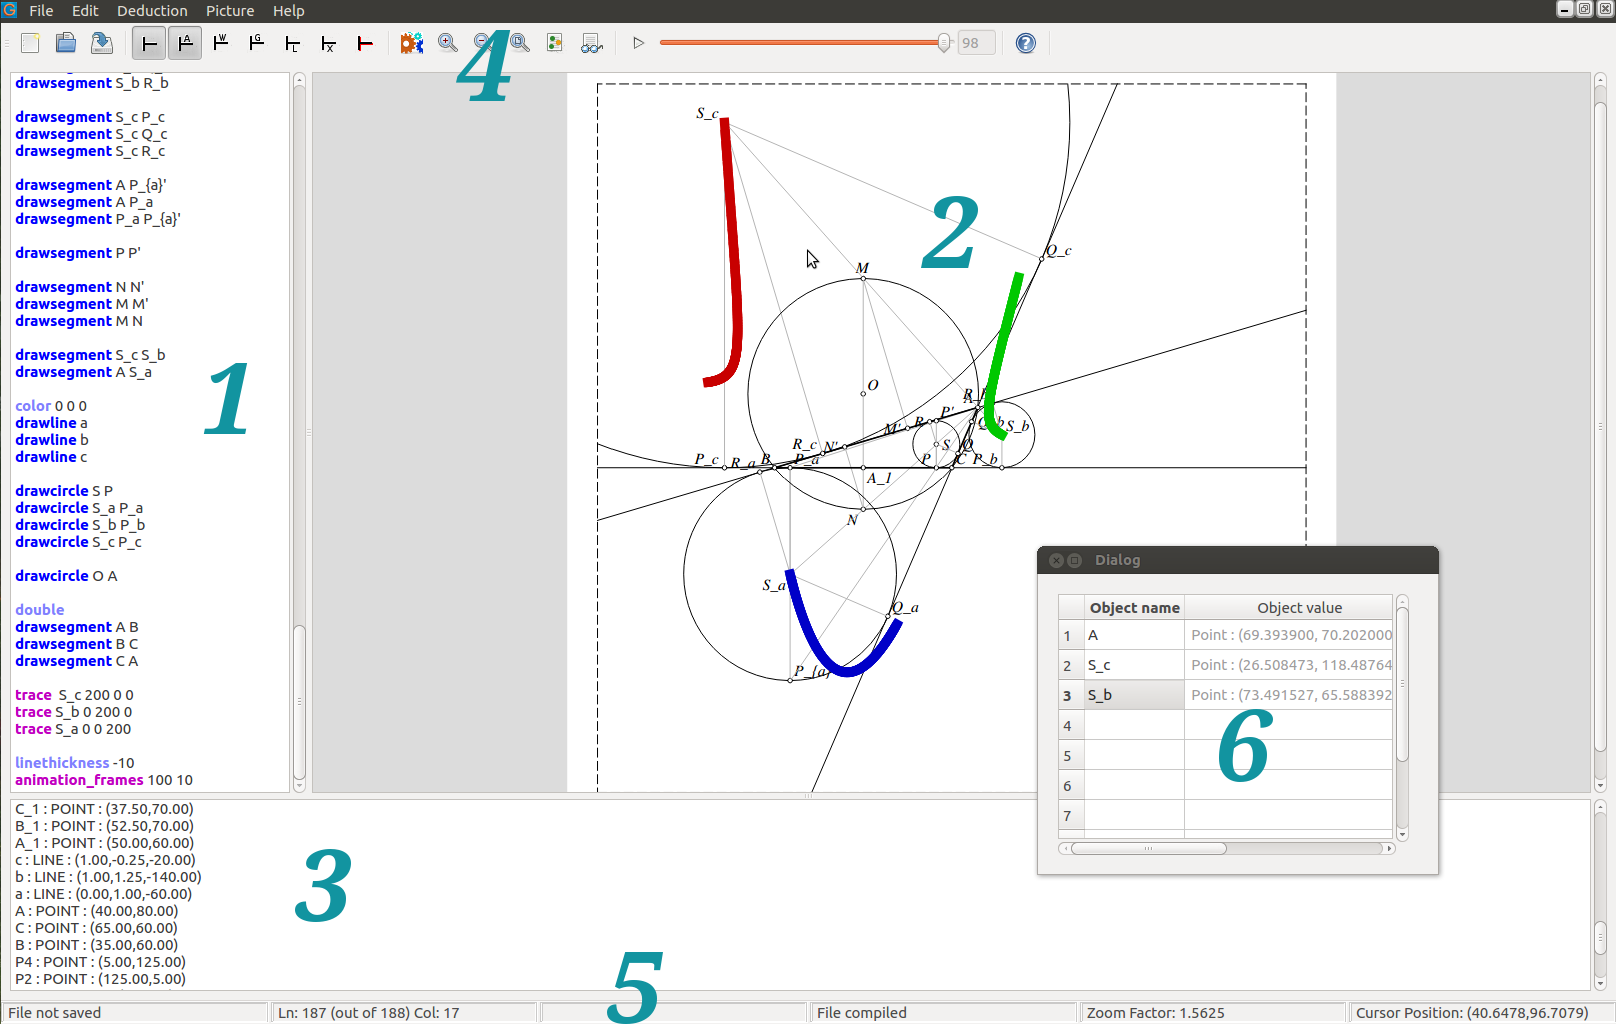
\includegraphics[width=0.9\textwidth]{figures/gclc-gui.png}
\end{center}
\caption{Screenshot of \gclcgui}
\label{fig:screenshot}
\end{figure}


\begin{description}
\item[Editor window] is provided here for writing source files (i.e.,
descriptions of a geometric construction) in it. It has standard
features which are expected from an text editor, find/replace, and
some additional features like coloring syntax and error/warning locating.

\index{point@{{\tt point}}}
\item[The Picture window] is used for showing the processed figure.
One can interactively work in this window by selecting and moving 
fixed points, zooming the picture, etc.
(Note: ``Fixed point'' is a point defined by {\sc gcl} command \verb|point|.)

\item[Debug/Log window] is a notifying window. It displays messages
about the status of the most recent operation such as compiling,
exporting etc.

\item[Menus and toolbars] are standard parts of almost every program with 
GUI program. There is a standard menu with a toolbar that provides shortcuts 
for menu items. Most items on the menu have an equivalent on some toolbar. 
The menu items can also be activated by appropriate keyboard shortcuts ---
for instance, Build (compiles a picture or builds animation) can be 
activated by the keys {\it Ctrl+B}.

\index{latex@\LaTeX}
\index{xml@{{\sc xml}}}
\begin{itemize}
\item The toolbar has a number of items, including those for
creating, opening and saving files, 
for zooming picture in and out, for theorem proving 
(for turning on and off the prover based on the area method,
for turning on and off the prover based on Wu's method,
for turning on and off the prover based on Gr\"obner bases method, 
for turning deduction control on and off,
for generating proofs in \LaTeX{}, 
for generating proofs in {\sc xml}.


\item The status bar displays some real-time information like
current line and column in editor window, current $x$ and $y$ coordinates of
the mouse pointer in the picture window, whether the file has been saved
or processed, and the zoom factor.
\end{itemize}

\end{description}


%----------------------------------------------------------------
\section{Features for Interactive Work}
%----------------------------------------------------------------


\begin{description}
\item[Creating/Opening:] In the beginning, one can created a new or open an 
existing \verb|*.gcl| file. From the {\it File} menu, select the item 
{\it New} and the blank new document window should appear. Type a few 
{\sc gcl} commands in the editor window. For instance, try this set of commands:

\begin{verbatim}
    point A 20 20
    point B 90 30
    point C 40 90

    drawsegment A B
    drawsegment B C
    drawsegment C A

    cmark_b A
    cmark_b B
    cmark_t C
\end{verbatim}

If you are not familiar with {\sc gcl}, explore some of the samples
and learn about commands of {\sc gcl}.

\item[Editing:] You can type {\sc gcl} commands in the editor window just
like in any other programming language.

\item[Building:] After entering of the source, select the
item {\it Build} from the {\it Picture} menu and start the 
compilation and building of the picture.
If there were no errors, a figure corresponding to the description
given by the source code will appear in the picture window (see
Figure \ref{fig:building}).

\begin{figure}[h]
\begin{center}
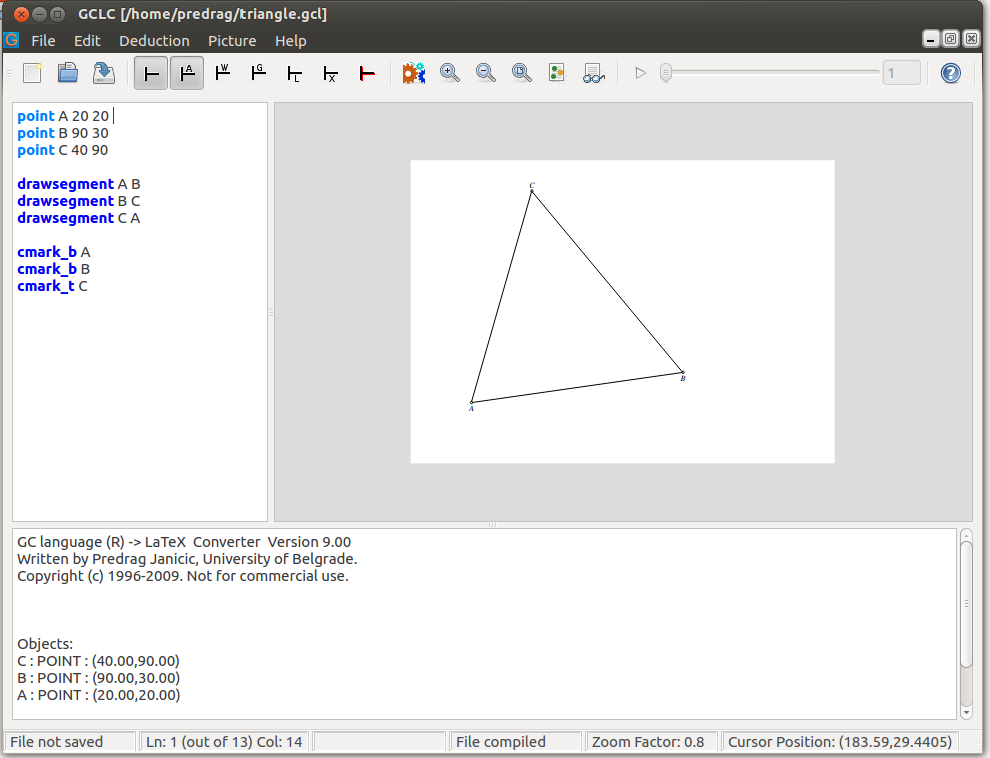
\includegraphics[width=0.9\textwidth]{figures/freePoints1.png}
\end{center}
\caption{After building the image}
\label{fig:building}
\end{figure}


\item[Modifying the picture:] Modifying the figure can be achieved by 
editing the source manually (which gives more control over the picture),
or by moving ``free'' points directly on the picture. After successful 
compilation, you can select the item {\it Show Free Points} from the 
{\it Picture} menu. Now, every free point will have a green circular
mark which can be selected (picked-up) and dragged to another position
(also changing the coordinates of the point in the editor).
In a similar way, destination points for animations can be dragged 
(while they have orange circular marks) (see Figure \ref{fig:selectedpoints}).

\begin{figure}[h]
\begin{center}
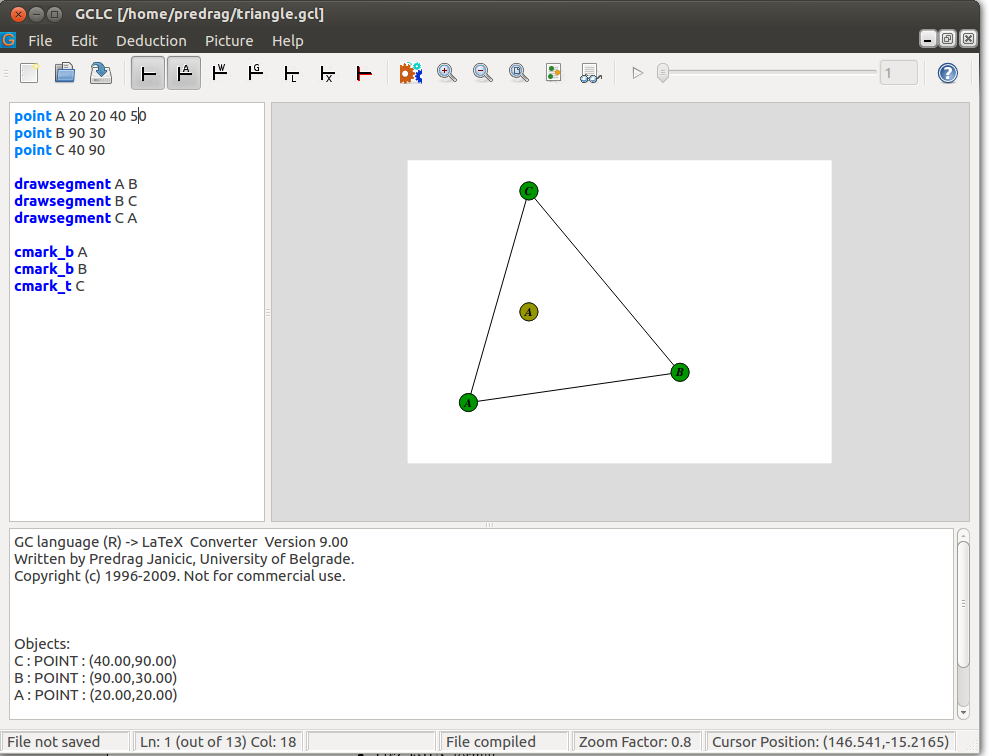
\includegraphics[width=0.9\textwidth]{figures/freePoints2.png}
\end{center}
\caption{Moving a fixed point}
\label{fig:selectedpoints}
\end{figure}

\index{export!to \LaTeX{}}
\index{export!to Ti{\em k}Z}
\index{export!to {\sc eps}}
\index{export!to {\sc svg}}
\index{export!to {\sc xml}}
\index{export!to bitmap}
\index{latex@\LaTeX}
\index{tikz@Ti{\em k}Z}
\index{PSTricks}
\index{bitmap}
\index{eps@{{\sc eps}}}
\index{xml@{{\sc xml}}}
\index{svg@{{\sc svg}}}
\item[Export:] GUI GCLC can export a compiled picture (or a particular
frame from an animation) to the following formats:
\begin{itemize}
    \item simple \LaTeX{} format (supported by \verb|gclc.sty|
    \item PSTricks \LaTeX{} format
    \item Ti{\em k}Z \LaTeX{} format
    \item Bitmap
    \item {\sc eps} (Encapsulated PostScript)
    \item {\sc svg} (Scalable Vector Graphics)
    \item raster formats: bitmap, PNG, JPG
    \item {\sc xml} (textual description of the figure given as {\sc xml} file).
\end{itemize}

    Also, an animation can be exported to a sequence of bitmaps
    (which can be further used for making animations by some other
    tool). These features are available in the {\it File/Export} menu.
    More about export options can be found in Chapter \ref{chapter:export}.

\index{import!from JavaView}
\index{JavaView}
\item[Import:] GUI \gclc can import JavaView .jvx files. This feature is
available in the {\it File/Import} from menu.

\index{latex@\LaTeX}
\index{xml@{{\sc xml}}}
\item[Theorem proving:] Options for the built-in theorem proving can
be accessed via the option group {\it Source} or via the {\it Source
toolbar}. If the source file contains a conjecture, \gclc will
automatically invoke the built-in theorem prover, if the option
{\it Theorem proving} is checked (i.e., if this button is turned on).
If the option {\it Deductive control} is checked, when a run-time
error occurs (during processing the source), \gclc will run the
prover to check whether this error occurs in all situations (i.e.,
whether it is a deductive consequence of the given construction)
(see Section \ref{sec:verification}).
Theorem prover can generate proofs in \LaTeX{} and in {\sc xml} form.
If at least one of the options {\it Theorem proving} and
{\it Deductive control} is checked, then the options {\it Generate Proofs
in \LaTeX{}} and {\it Generate Proofs in {\sc xml}} can be selected.
If neither of these two options were selected, then the prover works
without generating files with the proofs.
More about the theorem proving and the deduction control can be
found in Chapter \ref{chapter:prover}.


\item[Miscellaneous:] GUI \gclc provides some additional useful
features, including 

\begin{itemize}
    \item Watch window: Gives information about type and values of
    specified objects in the generated picture or in any particular
    animation frame.
\end{itemize}

\end{description}


%----------------------------------------------------------------
\chapter{Exporting Options}
\label{chapter:export}
%----------------------------------------------------------------

\index{export}
On the basis of a (valid) figure description in the file \verb|in.gcl|,
a figure can be generated by the command-line version of \gclc using
the following command:

\begin{verbatim}
> gclc in.gcl out.pic -option
\end{verbatim}

\noindent
where \verb|out.pic| is the name of a resulting file (it can have any
extension, not necessarily \verb|.pic|), and \verb|-option| controls
the output format. If the option is omitted, the output format is
the simple \LaTeX{} format (supported by \verb|gclc.sty|).
For PSTricks \LaTeX{} format, \verb|-pst| is used,
for Ti{\em k}Z \LaTeX{} format, \verb|-tikz| is used,
for {\sc eps}, \verb|-eps| is used, for {\sc svg}, \verb|-svg| is
used, and for {\sc xml}, the option \verb|-xml| is used.
The command line version of \gclc does not support export to bitmap.
\index{latex@\LaTeX}
\index{tikz@Ti{\em k}Z}
\index{PSTricks}
\index{bitmap}
\index{xml@{{\sc xml}}}
\index{eps@{{\sc eps}}}
\index{svg@{{\sc svg}}}

Within the GUI version of \gclc, a picture exported in some of 
supported formats can be obtained by selecting one of the option 
available in the group {\it File/Export to...} (see Chapter 
\ref{chapter:GUI}). When exporting a particular frame of an
animation, traces are also saved to output files.

\index{comments}
File exported to vector formats (\LaTeX, {\sc svg}, {\sc xml})
contain comments --- explanations for portions of code for
easier understanding and modifying.

\index{export\_to\_latex@{{\tt export\_to\_latex}}}
By using the \verb|export_to...| \gclc commands, arbitrary text can
be exported directly to files containing specific vector formats
(\LaTeX, {\sc svg}, {\sc xml}).

Note that mathematical formulae written within a \gclc file
will be formatted properly only when exported to \LaTeX{} formats.
If a figure is exported to, say, {\sc eps} format, it will
not have properly formatted formulae. In order to obtain an {\sc eps}
file with properly formatted formulae, one must first export the
file to \LaTeX{}, then process a \LaTeX{} file that contains
only this figure, then export the obtain document to a {\sc ps}
document, and then finally, convert the {\sc ps} to a {\sc eps} file.

\index{latex@\LaTeX}
\index{export!to \LaTeX{}}
When exported to \LaTeX{}, the text is printed in the math mode and
in the size \verb|footnotesize|.


%----------------------------------------------------------------
\section{Export to Simple \LaTeX{} format}
%----------------------------------------------------------------

By ''simple export \LaTeX{} format`` we mean the format based on
the \verb|gclc.sty| package. Good sides of this choice are:
there is just one file required (\verb|gclc.sty|), it can be
stored in standard folder for \LaTeX{} packages or in the current
folder, it can be easily shared with others to make \LaTeX{}
documents portable, or it can even be copied to \LaTeX{} documents
(since it is just few lines long). This package insignificantly
slows down processing \LaTeX{} documents that use it.
Bad sides of choosing this \LaTeX{} format are: in most systems
producing {\sc pdf} documents has to be performed via {\sc PostScript}
format. In addition, this format does not support some features
of \gclc, like filling polygons.


\subsection{Generating \LaTeX{} Files and {\sc gclc.sty}}

On the basis of a (valid) figure description in the file \verb|in.gcl|,
a picture in \LaTeX{} format can be generated by the command-line
version of \gclc using the following command:

\begin{verbatim}
> gclc in.gcl out.pic
\end{verbatim}

\noindent
where \verb|out.pic| is the name of a resulting file (it is not
necessary for it to have the extension \verb|.pic|).
If the extension of the input file is not given, then the assumed
extension is \verb|.gcl|.
If the name of the output file is not given, then the assumed name
is built from the input file name (e.g., \verb|in.pic|).

Within the GUI version of \gclc, a picture exported in \LaTeX{} format 
can be obtained by selecting the option {\it File/Export to.../LaTeX}.

The picture can be included in a \LaTeX{} document using the
command:

\begin{verbatim}
\input{figures/out.pic}
\end{verbatim}

\noindent
in appropriate position in your \LaTeX{} document.

\index{latexpackage@\LaTeX!package}
The package \verb|gclc| must be included (by \verb|\usepackage{gclc}|)
in the preamble of your document, or you can add the following lines
in the preamble:

\begin{verbatim}
\def\gclcpicture#1{%
   \def\gclcline##1##2##3##4##5##6##7{%
      \put(##1,##2){\special{em:point #1##3}}%
      \put(##4,##5){\special{em:point #1##6}}%
      \special{em:line #1##3,#1##6,##7mm}}}
\gclcpicture{1}
\end{verbatim}

If the command \verb|color| is used in the {\sc gcl} file, a \LaTeX{}
document including the corresponding picture (\verb|.pic| file) should
also use the package \verb|color|.\footnote{For convenience, the
package {\tt color.sty} (developed by other authors), is distributed
with \gclc.}


\subsection{Changing \LaTeX{} File Directly}

\index{latex@\LaTeX}
A position of the picture in your document can be changed by changing
(within any editor) appropriate parameters in the \gclc output file.
For example,

\begin{verbatim}
\begin{picture}(140.00,100.00)
\end{verbatim}

\noindent
can be changed to

\begin{verbatim}
\begin{picture}(180.00,100.00)(10.00,10.00)
\end{verbatim}

\noindent
in order to change picture dimensions and its position. (All values
in both input and output file are expressed in units of 1 millimeter.)


\subsection{Handling More Pictures on a Page}

If you want to put two or more pictures generated by \gclc on one
page, you might need to take care about point numbers, otherwise {\sc dvi}...
programs might report the warning \verb|duplicate point numbers| and
only your first picture on a page will be drawn correctly. This is
so because (many) {\sc dvi} programs can (in an appropriate mode)
address a limited number of points each of which has its own index.
These indices can go from 1 to 32767. If there are several pictures,
each of their points should have an index which is unique; indices
of points in different pictures thus could differ in the first digit.
So, before each, there should be one \verb|\gclcpicture| command with
the number of the picture (you can omit \verb|\gclcpicture{1}|
before the first picture):

\begin{verbatim}
\input{sample1.pic}
\gclcpicture{1}
\input{sample2.pic}
\end{verbatim}

This way, point indices are built by concatenating picture indices
and original point indices. Add command \verb|\gclcpicture{1}|
after a sequence of pictures supposed to be on the same page.
Note that if pictures have thousands of points this approach can fail
(for instance, if there are three pictures on a page, each with 3000
points).

There is also another solution for this problem: \gclc can create
pictures with indices of points starting with a given number. Therefore,
for example, if \gclc reports \verb|Ending point number: 99| after
successfully processing an input file, starting point number for the
second picture should be 100 or more:

\begin{verbatim}
> gclc in.gcl out.pic 100
\end{verbatim}

\noindent
If this parameter is omitted, the starting point number is 1.


\subsection{Batch Processing}

\index{latex@\LaTeX}
\index{batch processing}
If \gclc (the command line version) is called the option \verb|-b|,
then the batch processing is used. It expects a \LaTeX{} file with
blocks of \gclc commands, given in \verb|gclc| environment, and it
outputs a single \LaTeX{} file with \gclc commands replaced by
corresponding \LaTeX{} drawing commands (based on the \verb|gclc.sty|
style). This output file then should be processed (only) by \LaTeX{}
processor. If the option \verb|-b| is used, then all other options are
ignored (the theorem prover and deduction control are off, and only
exporting to \LaTeX{} is enabled).

The batch processing is used as in the following example:

\begin{verbatim}
> gclc in.tex out.tex -b
\end{verbatim}

If the extension of the input file is not given, then the assumed
extension is \verb|.tex|.
If the option \verb|-b| is used and if the name of the output
file is not given, then the assumed name is built from the input
file name (e.g., \verb|in-gclc.tex|).

For example, an input \LaTeX{} file (\verb|in.tex|) can be

\begin{verbatim}
\documentclass{article}
\usepackage{gclc}

\begin{document}

Here goes a triangle...

\begin{figure}[h]
    \begin{gclc}
        dim 100 35
        point A 10 10
        point B 80 10
        point C 30 30
        drawsegment A B
        drawsegment A C
        drawsegment B C
    \end{gclc}
\caption{Triangle}
\end{figure}

...and here goes a parametric curve...

\begin{gclc}
    dim 100 35
    ang_picture 0 0 100 35
    ang_origin 10 10
    ang_drawsystem
    ang_draw_parametric_curve x
        { 0; x<8; x+0.05}
        { x; sin(pow(x,2))*cos(x) }
\end{gclc}

\end{document}
\end{verbatim}



%----------------------------------------------------------------
\section{Export to PSTricks \LaTeX{} format}
%----------------------------------------------------------------
\index{export!to PSTricks}
\index{export!to \LaTeX{}}
\index{latex@\LaTeX}
\index{PSTricks}

PSTricks is a collection of PostScript-based \TeX{} macros
that is compatible with \LaTeX{} (but also most \TeX{} macro
packages, including plaint \TeX{}).
It enables creating high quality graphics in an inline manner.
PSTricks package is not distributed with \gclc.\footnote{It can
be found on {\tt http://tug.org/PSTricks}.}
Good sides of PSTricks choice are: it is very popular, very
expressive, it is understandable and can be relatively easily
modified by hand.
Bad sides of choosing this \LaTeX{} format are: it takes several
megabytes, it required installing dozens of \LaTeX{} packages,
it is impossible to share \LaTeX{} documents with those who
do not have PSTricks installed, it slows down a bit processing \LaTeX{}
documents that use it, in order to produce {\sc pdf} document,
an intermediate {\sc PostScript} document has to be generated.

On the basis of a (valid) figure description in the file \verb|in.gcl|,
a picture in PSTricks format can be generated by the command-line
version of \gclc using the following command:

\begin{verbatim}
> gclc in.gcl out.pst -pst
\end{verbatim}

\noindent
where \verb|out.pst| is the name of a resulting file.
If the extension of the input file is not given, then the assumed
extension is \verb|.gcl|.
If the option \verb|-pst| is used and if the name of the output
file is not given, then the assumed name is built from the input
file name (e.g., \verb|in.pst|).

Within the GUI version of \gclc, a picture exported in PSTricks format can be
obtained by selecting the option {\it File/Export to.../LaTeX-PSTricks}.

A picture in PSTricks format can be included in a \LaTeX{}
document using the command:

\begin{verbatim}
\input{out.pst}
\end{verbatim}

\noindent
in appropriate position in your \LaTeX{} document or the whole
picture in PSTricks format can be copied to the document
(the package \verb|pstricks| must be included.
\index{latexpackage@\LaTeX!package}

\index{latex@\LaTeX}
\index{batch processing}
Batch processing is supported for this format.
If \gclc (the command line version) is called the option \verb|-b|,
then the batch processing is used. It expects a \LaTeX{} file with
blocks of \gclc commands, given in \verb|gclc| environment, and it
outputs a single \LaTeX{} file with \gclc commands replaced by
corresponding \LaTeX{} PSTricks drawing commands. This output
file then should be processed (only) by \LaTeX{} processor. If
the option \verb|-b| is used, then all other options are ignored
(the theorem prover and deduction control are off).

The batch processing is used as in the following example:

\begin{verbatim}
> gclc in.tex out.tex -b -pst
\end{verbatim}



%----------------------------------------------------------------
\section{Export to Ti{\em k}Z \LaTeX{} format}
%----------------------------------------------------------------
\index{export!to Ti{\em k}Z}
\index{export!to \LaTeX{}}
\index{latex@\LaTeX}
\index{tikz@Ti{\em k}Z}

The {\sc pgf} package ({\sc pgf} is supposed to mean ,,portable
graphics format``), is a package for creating graphics in an
inline manner. It defines a number of \TeX{} commands that
draw graphics. Ti{\em k}Z is the natural frontend for {\sc pgf}.
It gives access to all features of {\sc pgf}, but it is intended
to be easy to use. The syntax is a mixture of {\sc metafont} and
{\sc pstricks} and some additional ideas.
The {\sc pgf} package, supporting Ti{\em k}Z format, is not
distributed with \gclc.\footnote{It can be found on
{\tt http://sourceforge.net/projects/pgf}.}
Good sides of Ti{\em k}Z choice are: it is very expressive,
it is understandable and can be relatively easily modified by hand,
it enables directly producing {\sc pdf} documents with figures
directly from the \LaTeX{} source (there is no need for {\sc PostScript}
intermediate step).
Bad sides of choosing this \LaTeX{} format are: it takes several
megabytes, it required installing dozens of \LaTeX{} packages,
it is impossible to share \LaTeX{} documents with those who
do not have {\sc pgf} installed, it slows down processing
\LaTeX{} documents that use it.

On the basis of a (valid) figure description in the file \verb|in.gcl|,
a picture in Ti{\em k}Z format can be generated by the command-line
version of \gclc using the following command:

\begin{verbatim}
> gclc in.gcl out.tkz -tikz
\end{verbatim}

\noindent
where \verb|out.tkz| is the name of a resulting file.
If the extension of the input file is not given, then the assumed
extension is \verb|.gcl|.
If the option \verb|-tikz| is used and if the name of the output
file is not given, then the assumed name is built from the input
file name (e.g., \verb|in.tkz|).

Within the GUI version of \gclc, a picture exported in Ti{\em k}Z format can be
obtained by selecting the option {\it File/Export to.../LaTeX-TikZ}.

A picture in Ti{\em k}Z format can be included in a \LaTeX{}
document using the command:

\begin{verbatim}
\input{out.tkz}
\end{verbatim}

\noindent
in appropriate position in your \LaTeX{} document or the whole
picture in Ti{\em k}Z format can be copied to the document
(the package \verb|tikz| must be included).
\index{latexpackage@\LaTeX!package}

\index{latex@\LaTeX}
\index{batch processing}
Batch processing is supported for this format.
If \gclc (the command line version) is called the option \verb|-b|,
then the batch processing is used. It expects a \LaTeX{} file with
blocks of \gclc commands, given in \verb|gclc| environment, and it
outputs a single \LaTeX{} file with \gclc commands replaced by
corresponding \LaTeX{} Ti{\em k}Z drawing commands. This output
file then should be processed (only) by \LaTeX{} processor. If
the option \verb|-b| is used, then all other options are ignored
(the theorem prover and deduction control are off).

The batch processing is used as in the following example:

\begin{verbatim}
> gclc in.tex out.tex -b -tikz
\end{verbatim}



%----------------------------------------------------------------
\section{Export to Raster-based Formats and Export to Sequences of Images}
%----------------------------------------------------------------

\index{export!to bitmap}
Within \gclcgui, there is available export to bitmap format
(option {\it File/Export to.../LaTeX}). The picture can be generated
for the following resolutions 75, 150, 300 and 600 {\sc dpi}.
There is also support for export to JPEG and PNG formats.

Within the GUI version, an animation can be exported to a sequence of
bitmaps (option File/Export to...) which can be further used for 
making animations by some other tool.


%----------------------------------------------------------------
\section{Export to {\sc eps} Format}
%----------------------------------------------------------------

\index{export!to {\sc eps}}
\index{eps@{{\sc eps}}}
On the basis of a (valid) figure description in the file \verb|in.gcl|,
a picture in {\sc eps} (Encapsulated PostScript Format) format can be
generated by the command-line version of \gclc using the following command:

\begin{verbatim}
> gclc in.gcl out.eps -eps
\end{verbatim}

\noindent
where \verb|out.eps| is the name of a resulting file.
If the extension of the input file is not given, then the assumed
extension is \verb|.gcl|.
If the option \verb|-eps| is used and if the name of the output
file is not given, then the assumed name is built from the input
file name (e.g., \verb|in.eps|).

Within the GUI version of \gclc, a picture exported in {\sc eps} 
format can be obtained by selecting the option {\it File/Export to.../EPS}.

A picture in {\sc eps} format can be included in a \LaTeX{}
document using the command:

\begin{verbatim}
\includegraphics[width=0.5\textwidth]{figures/out.eps}
\end{verbatim}

\noindent
in appropriate position in your \LaTeX{} document (the package
\verb|graphicx| must be included (by \verb|\usepackage{graphicx}|)
in the preamble of your document).
\index{latexpackage@\LaTeX!package}


%----------------------------------------------------------------
\section{Export to {\sc svg} Format}
%----------------------------------------------------------------

\index{export!to {\sc svg}}
\index{svg@{{\sc svg}}}
On the basis of a (valid) figure description in the file \verb|in.gcl|,
a picture in {\sc svg} (Scalable Vector Graphics) format can be
generated by the command-line version of \gclc using the following command:

\begin{verbatim}
> gclc in.gcl out.svg -svg
\end{verbatim}

\noindent
where \verb|out.svg| is the name of a resulting file.
If the extension of the input file is not given, then the assumed
extension is \verb|.gcl|.
If the option \verb|-svg| is used and if the name of the output
file is not given, then the assumed name is built from the input
file name (e.g., \verb|in.svg|).


Within the GUI version of \gclc, a picture exported in {\sc svg} 
format can be obtained by selecting the option {\it File/Export to.../SVG}.
A picture in {\sc svg} format can be directly open by modern
web browsers. For more details about {\sc xml} and {\sc svg}
see Chapter \ref{chapter:xml}.


%----------------------------------------------------------------
\section{Export to {\sc xml} Format}
%----------------------------------------------------------------

\index{export!to {\sc xml}}
\index{xml@{{\sc xml}}}
On the basis of a (valid) figure description in the file \verb|in.gcl|,
a textual description as {\sc xml} file can be generated by the
command-line version of \gclc using the following command:

\begin{verbatim}
> gclc in.gcl out.xml -xml
\end{verbatim}

\noindent
where \verb|out.xml| is the name of a resulting file.
If the extension of the input file is not given, then the assumed
extension is \verb|.gcl|.
If the option \verb|-xml| is used and if the name of the output
file is not given, then the assumed name is built from the input
file name (e.g., \verb|in.xml|).


Within the GUI version of \gclc, a figure description exported 
in {\sc xml} format can be obtained by selecting the option 
{\it File/Export to.../XML}. A figure description in {\sc xml} 
format can be directly open by modern web browsers. For more 
details about {\sc xml} and {\sc svg} see Chapter \ref{chapter:xml}.


%----------------------------------------------------------------
\section{Generating {\sc PostScript} and {\sc pdf} Documents}
%----------------------------------------------------------------

\index{pdf@{{\sc pdf}}}
\index{PostScript@{{\sc PostScript}}}
\LaTeX{} files with figures generated by \gclc should be normally
converted to {\sc dvi} format (by the \LaTeX{} processor), and then to
{\sc PostScript} (by some {\sc dvi} to {\sc PostScript} converter,
e.g., \verb|dvi2ps|).

\LaTeX{} files with figures generated by \gclc might not properly
get converted to {\sc pdf} documents in some environments (neither
by \LaTeX{} to {\sc pdf} processor, nor by {\sc dvi} to {\sc pdf}
converter, e.g., \verb|dvi2pdf|). If this is the case, then first
produce the {\sc dvi} file, then convert it to {\sc PostScript},
and then, finally, to {\sc pdf} (by some {\sc PostScript} to 
{\sc pdf} converter, e.g., \verb|ps2pdf|).



%----------------------------------------------------------------
\chapter{Theorem Proving}
\label{chapter:prover}
%----------------------------------------------------------------

\index{theorem prover}
\index{theorem prover!area method}
\index{theorem prover!Wu's method}
\index{theorem prover!Gr\"obner bases method}
There are three theorem provers built into \gclc{}:
\begin{itemize}
\item a theorem prover based on the Chou's {\em area method}\footnote{This
theorem prover based on the area method was developed in collaboration with
prof.~Pedro Quaresma, Department of Mathematics, University of
Coimbra, Portugal. This work was partially supported by CISUC/FCT,
Centro International de Matem\'atica (CIM), under the programme
``Research in Pairs'', while on visit to Coimbra University
under the Coimbra Group Hospitality Scheme.}
\cite{Chou93}; the prover produces traditional (i.e., geometric, not
algebraic, coordinate-based), readable proofs; the proofs are expressed in
terms of higher-level geometry lemmas and expression simplifications.

\item theorem provers based on the Wu's method \cite{wu1978,chou} and 
on the Gr\"obner bases method 
\cite{buchbergerPhd,groebner_bases_and_applications};\footnote{The main 
author of these theorem provers is Goran Predović (University of
Belgrade).} these provers are algebraic theorem provers; they are based 
on manipulating polynomials and they do not produce traditional geometrical 
proofs.
\end{itemize}

The theorem prover to be used is selected in the following way:
\begin{itemize}
\item in the command line version, by an appropriate parameter:
\verb|-a| for the area method (default), \verb|-w| for the Wu's method,
\verb|-g| for the Gr\"obner bases method.

\item in the GUI version, the theorem prover is selected by checking 
appropriate button in the toolbar or by checking the option 
{\it Deduction Control}.
\end{itemize}

All provers can prove a range of non-trivial theorems, including
theorems due to Ceva, Menelaus, Gauss, Pappus, Thales etc, but
they are still a subject of further improvements.

\index{prove@{{\tt prove}}}
\index{prooflevel@{{\tt prooflevel}}}
\index{prooflimit@{{\tt prooflimit}}}
\index{prover\_timeout@{{\tt prover\_timeout}}}
\index{theorem\_name@{{\tt theorem\_name}}}
Support for the provers involves only a few commands:
\begin{itemize}
\item \verb|prove| (for providing a conjecture);
\item \verb|prooflevel| (for setting the level of proof details);
\item \verb|prooflimit| (for setting maximal size of a proof).
\item \verb|prover_timeout| (for setting the timeout for the prover).
\item \verb|theorem_name| (for setting the theorem's name).
\end{itemize}

The provers work in both command line version and in GUI version
(and they do not use any specific functionalities of the GUI).
Proofs of theorems can be generated in \LaTeX{} or in {\sc xml}
form and saved in a file. For the area method, each deduction
step is accompanied by its semantics counterpart --- corresponding
numeric values in Cartesian plane.

The theorem provers are very efficient. Many conjectures are proved
in only milliseconds. However, some conjecture may take several seconds, 
several minutes, or in some specific cases even several hours. The 
maximal number of proof steps can be set by the command 
\verb|prooflimit|. The default value is 10000 proof steps.\footnote{On 
a modern PC computer, 10000 steps are performed in less then 1 minute.}
If the prover perform more proof steps, the proving process is stopped.
Similarly, the time available to the prover (in seconds) can be set by
the command \verb|prover_timeout|. The default value is 10 seconds.


\section{Introductory Example}
\label{sec:prover_example}

The theorem prover is tightly integrated into \gclc{}. This means that
one can use the prover to reason about a \gclc{} construction (i.e.,
about objects introduced in it), without any required adaptations
required for the deduction process. Of course, only the conjecture
itself has to be added.

The example \gclc{} code given in Figure \ref{midpoint-gclc} describes
a triangle and midpoints of two of
triangle's sides. This \gclc{} code produces the Figure \ref{fig:midpoint}.
It holds that the lines $AB$ and $A_1B_1$ are parallel and this can be
proved by the theorem prover. The conjecture ,,$AB$ and $A_1B_1$ are
parallel`` is given as argument to the \verb|prove| command in the
following way:

\verb|prove { parallel A B A_1 B_1 }|

At the end of the processing of the \gclc{} file, the theorem prover
is invoked; it can produce a proof in \LaTeX{} and in {\sc xml} form
(in the current directory) and, within the \gclc{} report, a report
about the proving process: whether the conjecture was proved or
disproved, data about CPU time spent, etc.
\index{prove@{{\tt prove}}}

\begin{figure}
\begin{verbatim}
point A 20 10
point B 70 10
point C 35 40

midpoint B_1 B C
midpoint A_1 A C

drawsegment A B
drawsegment A C
drawsegment B C
drawsegment A_1 B_1

cmark_b A
cmark_b B
cmark_t C
cmark_l A_1
cmark_r B_1

prove { parallel A B A_1 B_1 }
\end{verbatim}

\caption{Description of a triangle and midpoints of two of triangle's sides
and the conjecture of midpoint theorem}
\label{midpoint-gclc}
\end{figure}

\begin{figure}[ht]
\framebox[122mm][l]
{
\begin{minipage}[t]{120mm}
\input{figures/midpoint.tkz}
\end{minipage}
}
\caption{Illustration generated from the \gclc{} code from Figure
\ref{midpoint-gclc}}
\label{fig:midpoint}
\end{figure}


\section{Basic Sorts of Conjectures}
\label{sec:basic_conjectures}

Statements for the basic sorts of conjectures are given in the following table:

\begin{center}
\begin{tabular}{ll} \hline
points $A$ and $B$ are identical:   & \verb|identical A B| \\ \hline
points $A$, $B$, $C$ are collinear: & \verb|collinear A B C| \\ \hline
$AB$ is perpendicular to $CD$:      & \verb|perpendicular A B C D| \\ \hline
$AB$ is parallel to $CD$:           & \verb|parallel A B C D| \\ \hline
$O$ is the midpoint of $AB$:        & \verb|midpoint O A B| \\ \hline
$AB$ has the same length as $CD$:   & \verb|same_length A B C D| \\ \hline
points $A$, $B$, $C$, $D$ are harmonic: & \verb|harmonic A B C D |\\ \hline
\end{tabular}
\end{center}

All these sorts of conjectures can also be expressed in terms of
geometry quantities. Geometry quantities provide more general way
for stating conjectures.


\section{Geometry Quantities and Stating Conjectures}

The theorem prover deals with the following geometry quantities:
\begin{description}
\item[ratio of directed segments:] for four collinear points
$P$, $Q$, $A$, and $B$ such that $A \neq B$, it is the ratio
$\frac{\overrightarrow{PQ}}{\overrightarrow{AB}}$;
\item[signed area:] it is the signed area $S_{ABC}$ of a triangle
$ABC$ or the signed area $S_{ABCD}$ of a quadrilateral $ABCD$;
\item[Pythagoras difference:] for three points, $P_{ABC}$ is
defined as follows:
$$P_{ABC} = AB^2 + CB^2 - AC^2\;.$$
Pythagoras difference for four points, $P_{ABCD}$ is defined as follows:
$$P_{ABCD} = P_{ABD} - P_{CBD}\;.$$
\item[real number:] it is a real number, constant.
\end{description}

In \gclc{}, geometry quantities are written as in the following examples:
\vspace*{1mm}

\begin{center}
\begin{tabular}{|l|l|l|} \hline
ratio of directed segments &
$\frac{\overrightarrow{PQ}}{\overrightarrow{AB}}$ & \verb|sratio P Q A B| \\ \hline
signed area (arity 3) & $S_{ABC}$ & \verb|signed_area3 A B C|  \\ \hline
signed area (arity 4) & $S_{ABCD}$ & \verb|signed_area4 A B C D|  \\ \hline
Pythagoras difference (arity 3) & $P_{ABC}$ & \verb|pythagoras_difference3 A B C|  \\ \hline
Pythagoras difference (arity 4) & $P_{ABCD}$ & \verb|pythagoras_difference4 A B C D|  \\ \hline
\end{tabular}
\end{center}


A conjecture to be proved is given as argument to the \verb|prove|
command. It has to be some of the basic sorts of conjectures
(see Section \ref{sec:basic_conjectures}), or it has to be of the 
form $L=R$, where $L$ and $R$ are expressions over geometry quantities. 
The conjecture can involve geometry quantities (only) over points 
already introduced (by a subset of commands) within the current 
construction. Geometry quantities can be combined together into 
more complex terms by operators for addition, multiplication and 
division. Operators are written in textual form as in the following table:

\begin{center}
\begin{tabular}{|l|l|} \hline
$=$ & equality \\ \hline
$+$ & sum \\ \hline
$\cdot$ & mult \\ \hline
$/$ & ratio \\ \hline
\end{tabular}
\end{center}

The conjecture and all its subterms are written in prefix form, with
brackets if needed. For instance,
$$S_{A_1B_1A} = S_{A_1B_1B}$$
is given to be proved in the following way:

\begin{verbatim}
prove { equal { signed_area3 A_1 B_1 A }
              { signed_area3 A_1 B_1 B }
      }
\end{verbatim}

and
$$\left( \left( \frac{\overrightarrow{AF}}{\overrightarrow{FB}} \cdot
\frac{\overrightarrow{BD}}{\overrightarrow{DC}}\right) \cdot
\frac{\overrightarrow{CE}}{\overrightarrow{EA}}\right) =  1$$
is given to be proved in the following way:

\begin{verbatim}
prove { equal { mult { mult { sratio A F F B }
                            { sratio B D D C } }
                     { sratio C E E A } }
              1 }
\end{verbatim}

A range of geometry conjectures can be stated in terms of geometry
quantities. The representations for the basic sorts of conjectures
is are given in the following table:

\begin{center}
\begin{tabular}{lll} \hline
points $A$ and $B$ are identical   & iff & $P_{ABA}=0$ \\ \hline
points $A$, $B$, $C$ are collinear & iff & $S_{ABC}=0$ \\ \hline
$AB$ is perpendicular to $CD$      & iff & $P_{ACD}=P_{BCD}$ \\ \hline
$AB$ is parallel to $CD$           & iff & $S_{ACD}=S_{BCD}$ \\ \hline
$O$ is the midpoint of $AB$        & iff & $\frac{\overrightarrow{AO}}{\overrightarrow{OB}}=1$ \\ \hline
$AB$ has the same length as $CD$   & iff & $P_{ABA} = P_{CDC}$ \\ \hline
points $A$, $B$, $C$, $D$ are harmonic & iff & $\frac{\overrightarrow{AC}}{\overrightarrow{CB}}=\frac{\overrightarrow{DA}}{\overrightarrow{DB}}$ \\ \hline
\end{tabular}
\end{center}

Note that the command

\begin{verbatim}
prove { parallel A B A_1 B_1 }
\end{verbatim}

\noindent
(from Section \ref{sec:prover_example}) is equivalent to

\begin{verbatim}
prove { equal { signed_area3 A_1 B_1 A }
              { signed_area3 A_1 B_1 B }
      }
\end{verbatim}

The prover transforms the basic sorts of conjectures into statements
given in terms of geometric quantities: if a conjecture of a basic
sort is given, the very first step in the proof is its formulation
in terms of geometric quantities.


The conjecture can involve geometry quantities only over points and lines
already introduced within the current construction, and by using (only)
the following commands:

\begin{itemize}
\index{point@{{\tt point}}}
\item \verb|point|
\index{line@{{\tt line}}}
\item \verb|line|
\index{intersec@{{\tt intersec}}}
\item \verb|intersec|
\index{midpoint@{{\tt midpoint}}}
\item \verb|midpoint|
\index{med@{{\tt med}}}
\item \verb|med|
\index{perp@{{\tt perp}}}
\item \verb|perp|
\index{foot@{{\tt foot}}}
\item \verb|foot|
\index{parallel@{{\tt parallel}}}
\item \verb|parallel|
\index{translate@{{\tt translate}}}
\item \verb|translate|
\index{towards@{{\tt towards}}}
\item \verb|towards|
\index{online@{{\tt online}}}
\item \verb|online|
\end{itemize}

The prover cannot prove conjectures about object constructed by using
some other commands. For instance, if a line $a$ is constructed by
the command \verb|bis|, then the prove cannot prove conjectures involving
$a$ or involving points constructed by using $a$.


\section{Area Method}
\label{sec:area_method}

\index{theorem prover!area method}
One of the theorem prover built into \gclc{} is based on the algorithm
described in \cite{Chou93}. The basic idea of the algorithm is to express
a theorem in terms of geometry quantities, to eliminate (by appropriate
lemmas) all occurrences of constructed point and to simplify the
expression, yielding a trivial equality.


\subsection{Underlying Constructions}

In \cite{Chou93}, a construction is expressed in terms of
commands \verb|INTER|, \verb|PRATIO|, \verb|TRATIO| and \verb|FOOT|:

\begin{description}

\item[{\tt INTER Y ln1 ln2}]: Point $Y$ is the intersection of line
  $ln_1$ and line $ln_2$.

\item[{\tt PRATIO Y W U V r}]: Point \verb|Y| is a point such that
$\overline{WY}=r\overline{UV}$, where $r$ is a real number.

\item[{\tt TRATIO Y U V r}]: Point $Y$ is a point on line $l$,
such that $r = \frac{UY}{UV}$, where $r$ is a real number
and $l$ is a line such that $U$ lies on $l$ and $l$ is perpendicular to $UV$.

\item[{\tt FOOT Y P U V}]: Point $Y$ is a foot from $P$ to line $UV$
(i.e., $YP$ is perpendicular to $UV$ and $Y$ lies on $UV$.
\end{description}

For each point $X$ constructed by the above constructions and for each
geometry quantity $g$ involving $X$, there is a suitable lemma that
enables replacing $g$ by an expression with no occurrences of $X$.
Thanks to these lemmas, all constructed points can be eliminated
from the conjecture.

\subsection{Integration of Algorithm and Auxiliary Points}

In order to be tightly integrated into \gclc{}, the prover uses
standard \gclc{} construction commands and, if needed, transforms them
internally into form required by the algorithm and/or introduces
some auxiliary points:

\begin{description}
\item[{\tt midpoint}] is expressed in terms of \verb|PRATIO|, it
does not introduce new points;

\item[{\tt foot}] is expressed in terms of \verb|FOOT|, it
does not introduce new points;

\item[{\tt med}] introduces two auxiliary points: for instance,
\verb|med m A B| introduce a point $M_m$ as the midpoint of $AB$
and a point $T_m$ on the bisector of $AB$ (such that
${\tt TRATIO \;\; T_m \;\; M_m \;\; A \;\; 1}$); the line $m$
is then determined by the points $M_m$ and $T_m$;

\item[{\tt perp}] introduces one auxiliary point: if $A$ lies
on the line $q$, then \verb|perp p A q| introduces a point $T_p$
on a line perpendicular to $q$ (such that 
${\tt TRATIO \;\; T_p \;\; A \;\; Q_1 \;\; 1}$;
where the line $q$ is determined by points $Q_1$ and $Q_2$);
in this case, the line $p$ is determined by the points $A$ and $T_p$;
if $A$ does not lie on the line $q$, then \verb|perp p A q| introduce
a point $F_p$ which is a foot of the normal from $A$ to the line $q$;
in this case, the line $p$ is determined by the points $A$ and $F_p$;

\item[{\tt parallel}] introduces one auxiliary point: for instance,
{\tt parallel p A q} introduces a point $P_p$ on a line parallel to
$q$ (such that ${\tt PRATIO \;\; P_p \;\; A \;\; Q_1 \;\; Q_2 \;\; 1}$;
the line $p$ is then determined by the points $A$ and $P_p$;

\item[{\tt translate}] is expressed in terms of \verb|PRATIO|,
it does not introduce new points;

\item[{\tt towards}] is expressed in terms of \verb|PRATIO|,
it does not introduce new points;

\item[{\tt online}] is expressed in terms of \verb|PRATIO|,
it does not introduce new points, but introduces a (indeterminate)
constant $r$: for instance, \verb|online X A B| is interpreted
as ${\tt PRATIO \;\; X \;\; A \;\; A \;\; B \;\; r}$.
\end{description}

Definitions of auxiliary points are given at the beginning of the proof.


\subsection{Non-degenerative Conditions and Lemmas}

Some constructions are possible only if certain conditions are met. For
instance, the construction \verb|inter X a b| is possible only if the
lines \verb|a| and \verb|b| are not parallel. For such constructions
{\em non-degenerative conditions} are store for future possible use and
listed at the end of the proof.

Some non-degenerative conditions can also be introduced during the
proving process:
\begin{itemize}
\item some lemmas have two cases (for instance, ,,if $A$ belongs to
$CD$`` and ,,if $A$ does not belong to $CD$``); if a condition for
one case can be proved (as a lemma), then that case is applied,
otherwise, a condition for one case (the one of the form $L \neq R$)
is assumed and introduced as a non-degenerative condition.
\item in the cancellation rule, if all summands on both sides of
the equality have the same multiplication factor $X$, the rule tries
to prove (as a lemma) that $X=0$; if this fails, a condition $X \neq 0$
is assumed and introduced as a non-degenerative condition and
the equality is cancelled by $X$.
\end{itemize}

Lemmas are being proved as separate conjectures, but, of course,
sharing the construction and non-degenerative conditions with outer
context.


\subsection{Structure of Algorithm}

The algorithm has one main {\em while} loop --- it process the
sequence of all (relevant) constructions in backward manner
(from last to first construction step) and transforms the
current goal as follows:

\begin{itemize}
\item the current goal is initially the given conjecture;
\item {\em while} there are construction steps do:
\begin{itemize}
\item apply geometric simplifications to the current goal;
\item apply algebraic simplifications to the current goal;
\item if the current construction step introduce a new point $P$,
then eliminate (using the elimination rules) one of occurrences
of $P$ (from the current goal) and go to the top of the while
loop; otherwise, go to next construction step.
\end{itemize}
\item apply geometric simplifications to the current goal;
\item apply algebraic simplifications to the current goal.
\item if the current goal is a equality trivially true, then
the conjecture has been proved, if the current goal is a
equality trivially false, then the conjecture has been disproved,
otherwise, the conjecture has been neither proved nor disproved.
\end{itemize}

The reasoning steps, as seen from the above overall algorithm,
are divided into three groups:
\begin{description}
\item[algebraic simplifications:] applies simplification rewrite
rule (not directly related to geometry) such as:

\begin{eqnarray*}
x + 0 & \rightarrow & x \\
0 + x & \rightarrow & x \\
x \cdot 1 & \rightarrow & x \\
x \cdot 0 & \rightarrow & 0 \\
\frac{x}{y}+\frac{u}{v} & \rightarrow & \frac{x\cdot v+ u\cdot y}{y\cdot v} \\
\ldots & &
\end{eqnarray*}

\item[geometric simplifications:] applies simplification rewrite
rule, directly related to geometry quantities such as:

\begin{eqnarray*}
S_{AAB} & \rightarrow & 0 \\
S_{ABC} & \rightarrow & S_{BCA} \\
P_{AAB} & \rightarrow & 0 \\
\ldots & &
\end{eqnarray*}

\item[elimination simplifications:] applies elimination lemmas for
eliminating constructed points for the current goal; for instance,
if the point $Y$ is introduced by as the intersection of lines
$l_1$ (determined by $U$ and $V$) and $l_2$ (determined by $P$
and $Q$), then $Y$ can be eliminated from expression of the form
$\frac{\overrightarrow{AY}}{\overrightarrow{CD}}$ using the
following equality:
$$\frac{\overrightarrow{AY}}{\overrightarrow{CD}} =
\left\{\begin{array}{ll}
\frac{S_{APQ}}{S_{CPDQ}} \;, & \mbox{if $A \in UV$} \\
\frac{S_{AUV}}{S_{CUDV}} \;, & \mbox{if $A \not\in UV$}
\end{array}\right.$$
\end{description}


Full details about all used lemmas and rewrite rules are given in
the technical report ``Framework for constructive geometry (based
on the area method)'' (written by Pedro Quaresma and Predrag Janičić)
\cite{Quaresma06}. This technical report is a part of \gclc{} distribution.


\subsection{Scope}

\index{point@{{\tt point}}}
The theorem prover can prove {\em any} geometry theorem expressed in
terms of geometry quantities, and involving only points introduced by
using the commands \verb|point|, \verb|line|, \verb|intersec|,
\verb|midpoint|, \verb|med|, \verb|perp|, \verb|foot|, \verb|parallel|,
\verb|translate|, \verb|towards|, \verb|online|.  This can be proved
following the ideas from \cite{Chou93}. However, some of the proofs
can be very long and can take lot of time.


\section{Wu's Method and Gr\"obner Bases Method}

\index{theorem prover!Wu's method}
\index{theorem prover!Gr\"obner bases method}
One of the theorem prover built into \gclc{} is based on the Wu's
method \cite{wu1978,chou} and one is based on the Gr\"obner bases
method \cite{buchbergerPhd,groebner_bases_and_applications}. These
methods are algebraic methods and they prove geometrical statements
by manipulating polynomials corresponding to the constructions and
given conjectures. These methods can also detect non-degenerative
conditions, described in Section \ref{sec:area_method}.


\section{Prover Output}

Whenever there was a conjecture given in the input {\sc gcl} file,
the prover produces a short report.
The prover can also generate proofs in \LaTeX{} format, or in
{\sc xml} format. The level of details given in generated proof
can be controlled by the user.


\subsection{Prover's Short Report}

The prover produces a short report (if there was a conjecture given
in the {\sc gcl} file). In the command line version, this short
report is shown and written in the log file, while the GUI version shows
this report in its output window. For the area method, this report
consists of information on number of steps performed, on CPU time
spent and whether or not the conjecture has been proved. For example:

\begin{verbatim}
Number of elimination proof steps:      3
Number of geometric proof steps:        6
Number of algebraic proof steps:       23
Total number of proof steps:           32

Time spent by the prover: 0.002 seconds
The conjecture successfully proved.
The prover output is written in the file ceva_proof.tex.
\end{verbatim}



\subsection{Controlling Level of Output}

\index{prooflevel@{{\tt prooflevel}}}
For the area method, the level of generated proof output is controlled
by the command \verb|prooflevel|. This command has one argument (an
integer from 0 to 7) which provides the output level:

\begin{itemize}
\item[0]: no output (except the statement);
\item[1]: elimination steps plus grouped geometric steps and algebraic steps;
\item[2]: elimination steps plus geometric steps plus grouped algebraic steps;
\item[3]: as level 2, plus statements of lemmas;
\item[4]: as level 3, plus elimination steps plus grouped geometric steps
and algebraic steps in lemmas;
\item[5]: as level 4, plus geometric steps in lemmas;
\item[6]: as level 5, plus algebraic steps at proof level 0;
\item[7]: as level 6, plus algebraic steps in lemmas.
\end{itemize}

The default output level is 1.

For the algebraic theorem provers, the output is always given
in a standard form and the command \verb|prooflevel| is ignored.


\subsection{Proofs in \LaTeX{} format}

\index{prove@{{\tt prove}}}
\index{export!to \LaTeX{}}
\index{export!to {\sc eps}}
\index{latex@\LaTeX}
\index{eps@{{\sc eps}}}

The proof in \LaTeX{} form is generated by the command line version
of \gclc, if the option \verb|-eps| (for export to {\sc eps} format)
is used, or, if there no export option is used (when the figure
is exported to \LaTeX{} format).

The proof in \LaTeX{} form is generated by the GUI version of \gclc, 
if the option {\it Deduction/Proof Export to LaTeX} is checked.

In these cases, the proof is exported to the file \verb|name_proof.tex|
(in the current directory, \verb|name| is the name of the input file).
If there is no \verb|prove| command within the construction, then
the file with a proof will not be created.

For proofs generated by the area method, at the beginning of the proof,
the auxiliary points are defined, for instance:
\vspace*{2mm}

\noindent
\framebox[122mm][l]
{
\begin{minipage}[t]{117mm}
Let $M_{a}^{0}$ be the midpoint of the segment $BC$.

Let $T_{a}^{1}$ be the point on bisector of the segment
$BC$ (such that {\tt TRATIO} $T_{a}^{1}$ $M_{a}^{0}$ $B$ $1$).

\end{minipage}
}
\vspace*{2mm}

The proof consists of {\em proof steps}. In each proof step, the
current goal is changed. For each proof step, there is an explanation
and (optionally) its semantics counterpart. This semantic information
is calculated for concrete points used in the construction (note that
these coordinates are never used in the proof itself); it can serve as
a semantic test, especially for conjectures for which is not
known whether or not they are theorems. Proof step are enumerated.
For example:
\vspace*{2mm}

\noindent
\framebox[122mm][l]
{
\begin{minipage}[t]{117mm}
\begin{tabular}{lll}
$\!\!\!\!\! \left( \left( \frac{\overrightarrow{AF}}{\overrightarrow{FB}} \cdot  \frac{\overrightarrow{BD}}{\overrightarrow{DC}}\right) \cdot  \frac{\overrightarrow{CE}}{\overrightarrow{EA}}\right)$ & $\!\!\!\!\!$= 1 & $\!\!$ by the statement (value 1=1) \\
$\!\!\!\!\! \left( \left( \left( -1  \cdot  \frac{\overrightarrow{AF}}{\overrightarrow{BF}}\right) \cdot  \frac{\overrightarrow{BD}}{\overrightarrow{DC}}\right) \cdot  \frac{\overrightarrow{CE}}{\overrightarrow{EA}}\right)$ & $\!\!\!\!\!$= 1 & $\!\!$ by geometric simplifications (value 1=1)

\end{tabular}
\end{minipage}
}
\vspace*{2mm}

Lemmas are proved within the main proof (making nested proof levels),
and the beginning and the end of a proof for a lemma is marked by a
horizontal solid line.

\index{QED@{{\tt Q.E.D.}}}
At the end of a proof, it is reported if the conjecture is proved
(``Q.E.D.'' --- lat.~Quod Erat Demonstrandum --- which was required 
to prove), if the conjecture is disproved (if it was shown that it 
is invalid), or neither of these two.

At the end of the main proof all non-degenerative conditions are
listed. For instance:
\vspace*{2mm}

\noindent
\framebox[122mm][l]
{
\begin{minipage}[t]{117mm}
$S_{M_{a}^{0}M_{b}^{2}T_{b}^{3}}\neq S_{T_{a}^{1}M_{b}^{2}T_{b}^{3}}$
i.e., lines $M_{a}^{0}T_{a}^{1}$ and $M_{b}^{2}T_{b}^{3}$ are not
parallel (construction based assumption)

\end{minipage}
}
\vspace*{2mm}

For proofs generated by the Wu's and Gr\"obner bases method, the
output consist of a summary of processing steps over the relevant
set of polynomials.

See one complete example in the appendix (Section \ref{sec:ceva}).


\subsubsection*{Modifying \LaTeX{} Output}

\index{latexpackage@\LaTeX!package}
The prover exports proofs in \LaTeX{} form. These \LaTeX{} files
require \LaTeX{} package \verb|gclcproof.sty|.

Once generated, the proof in \LaTeX{} form can still be parameterized.
Namely, data in the file can be formatted in several ways, giving
different layouts. Also, semantics part can be omitted.
Parameters for proof formatting are given as options for the
package \verb|gclcproof.sty|. There are three parameters:

\begin{description}
\item[style:] defines the layout; available choices are:
\begin{itemize}
\item \verb|portrait| --- uses the package \verb|longtable| to
generate a multi-page table.\footnote{For convenience, the required
packages {\tt breqn.sty}, {\tt flexisym.sty}, {\tt mathstyle.sty},
{\tt cmbase.sim} (developed by other authors), are distributed with \gclc.
The packages {\tt longtable.sty}, {\tt lscape,sty}, {\tt amsmath.sty}
(developed by other authors) are not distributed with \gclc,
but are widely available, most often as part of a \TeX{} distribution.}

\item \verb|portraitbreqn| --- uses the package \verb|breqn| to try to
break the equations. Problems with extra large fractions.

\item \verb|landscape| --- uses the packages \verb|lscape|, \verb|amsmath|
(with option \verb|leqno|), and \verb|breqn|, to generate the list of
equations in landscape mode, with numbers on the left, and with
automatic equation breaking.
\end{itemize}

The default value for style is \verb|portrait|.

\item[size:] defines the font size in the proof. It uses the
\LaTeX{} font size names of, from \verb|tiny| up to \verb|large|.
 The default value is \verb|small|.

\item[semantic values:] controls if the semantics values will be shown.
If the option \verb|semantics| is used, the semantic values of both sides
of equations will be shown. The default value is NULL, i.e., without
any value. The semantics values are only generated by the area method.
\end{description}


According to the above,

\verb|\usepackage{gclcproof}|

\noindent
is equivalent to

\verb|\usepackage[portrait,small]{gclcproof}|

\noindent
(which gives a proof in portrait style, small size, without semantics style).

For example,

\begin{itemize}
\item \verb|\usepackage[tiny]{gclcproof}|

\noindent
retains the portrait mode (default value), but decrease the size
of the fonts used in the proof to tiny. No semantic values displayed.

\item
\verb|\usepackage[portraitbreqn,sematics]{gclcproof}|

\noindent
uses the \verb|breqn| package of the AMSTeX to try to break automatically
the equations. Portrait form, small size fonts, semantic values
displayed. Note: the \verb|breqn| package may fail (not being able to
process the document) if the proof contains large fractions, \verb|breqn|
it is unable to break them into lines.

\item
\verb|\usepackage[landscape]{gclcproof}|

\noindent
uses the packages \verb|lscape|, \verb|amsmath| (with option \verb|leqno|),
and \verb|breqn| to produce a proof in landscape mode. It is the mode that
provides the larger environment for proofs, so in some proofs it will be
the only one to be able to display the proofs without overlapping of
the different elements. Note: the rotation of the proof to
landscape mode it is done with Postscript specials, so it may not
display properly in some viewers. The size of the fonts it is
small, and the sematic values are not displayed.
\end{itemize}

In the generated proofs, there is always \verb|\usepackage{gclcproof}|
used (in the preamble) and the layout can be changed by using
options for this command, as discussed above.


\subsection{Proofs in {\sc xml} format}

\index{export!to {\sc xml}}
\index{export!to {\sc svg}}

\index{prove@{{\tt prove}}}
\index{xml@{{\sc xml}}}
\index{svg@{{\sc svg}}}
The proof in {\sc xml} form is generated by the command line version
of \gclc, if the option \verb|-xml| (for export to {\sc xml} format)
or if the option \verb|-svg| (for export to {\sc svg} format)
is used.

The proof in {\sc xml} form is generated by the GUI version of \gclc, 
if the option {\it Deduction/Proofs Export to XML} is checked.

In these cases, the proof is exported to the file \verb|name_proof.xml|
(in the current directory, \verb|name| is the name of the input file).
If there is no \verb|prove| command within the construction, then
the file with a proof will not be created.

Proofs stored in {\sc xml} are formatted analogously as
in \LaTeX{} format.

The proofs in {\sc xml} format fulfil restrictions posed by
\verb|GeoCons_proof.dtd| (as stated in the
line \verb|<!DOCTYPE figure SYSTEM "GeoCons_proof.dtd">| in each of
these files). For any {\sc xml} file, it can be checked if it meets
these restrictions. It can be done using a {\sc xml} processor, such
as \verb|AltovaXML| (copyrighted by Altova GmbH). For instance:

\begin{verbatim}
> AltovaXML /v GeoCons_proof.dtd thm_proof.xml
\end{verbatim}

\noindent
verifies if the file \verb|thm_proof.xml| is valid.

A proof in {\sc xml} format (valid with respect to \verb|GeoCons_proof.dtd|)
can be converted to a {\scshape html} form, for example:
{\footnotesize
\begin{verbatim}
>AltovaXML.exe /xslt1 GeoCons_proof.xsl /in thm_proof.xml /out thm_proof.html
\end{verbatim}}

A file with a proof in {\sc xml} format can also be open directly
by web browsers. See one example in the appendix (Section \ref{sec:ceva}).

For more details about proofs represented in {\sc xml} format,
see Chapter \ref{chapter:xml}.


% --------------------------------------------------------------------------------
\section{Automatic Verification of Regular Constructions}
\label{sec:verification}
% --------------------------------------------------------------------------------

\index{deductive verification}
A geometrical construction is associated with some fixed points (with 
concrete Cartesian coordinates). In such environments, some 
constructions (e.g., if they attempt to use intersection of parallel
lines), but the question if such construction is always illegal or
it is illegal only for given particular fixed points is not trivial
(if a construction is never illegal, i.e., if it is always possible,
we will call it {\em regular}). For answering such question, one has
to use deductive reasoning, and not only semantic check for the special 
case. Consider one simple example: given (by Cartesian coordinates)
three fixed distinct points $A$, $B$, $C$, we can construct a point $D$
as an image of the point $C$ in translation ${\cal T}_{AB}$ (in terms 
of \gclc commands: \verb|translate D A B C|); later on, if we try to 
construct an intersection of lines $AC$ and $BD$, we will discover 
that there is no such intersection (since these two lines are parallel). 
This holds not for some specific points $A$, $B$, $C$, with $D$ 
determined as above, but for all triples of points $A$, $B$, $C$. 
So, this construction is illegal, and moreover, it is illegal not 
only for a given special case, but always.

The system for automated testing whether a construction is regular or
illegal is built into \gclc and is based on the built-in theorem provers.
All built-in theorem provers can be used for this purpose.
This verification mechanism can be switched on or off:
\begin{itemize}
\item in the command line version, the verification mechanism is turned
on by using the option \verb|-d|.
\item in the GUI version, the verification mechanism is turned on by checking
the button {\it Deduction Control} in the toolbar or the option
{\it Deduction/Deduction Control}.
\end{itemize}

\index{latex@\LaTeX}
\index{xml@{{\sc xml}}}
If the verification mechanism is turned on, while processing the input file
(with a description of a geometrical construction), \gclc provides to the
theorem prover all construction steps performed. When \gclc encounters a
construction step that cannot be performed (e.g., two identical points
do not determine a line), it reports that the step is illegal with
respect to a given set of fixed points, and then it invokes the theorem 
prover. The prover is run on the critical conjecture (e.g., it tries to 
prove that two points are identical) and, if successful, it reports that 
the construction step is always illegal/impossible. The prover generates 
the proof for the critical construction:

\begin{itemize}
\item in the command line version: in the format selected for conjectures
(see Chapter \ref{chapter:export});
\item in the GUI version: in \LaTeX{} and {\sc xml} format if the options,
respectively, {\it Proof Export to \LaTeX{}} and {\it Proof Export to 
{\sc xml}} are checked.
\end{itemize}


\paragraph{Realm.}
\label{sec:realm}

The verification deductive-check system currently covers the following 
critical commands and constructions:

\begin{description}
\item[{\tt line}] --- construction of a line given two points (error if
the two points are identical);
\item[{\tt med}] --- construction of a segment-bisector given two endpoints
(error if the two points are identical);
\item[{\tt bis}] --- constructing an angle-bisector of the angle determined 
by three points $A$, $B$, $C$ (error if $A$ and $B$, or $C$ and $B$ are 
identical);
\item[{\tt intersec}] --- constructing an intersection of lines $a$ and $b$
(error if the two lines are parallel);
\item[{\tt angle}] --- calculating an angle determined by three points 
$A$, $B$, $C$ (error if $A$ and $B$, or $C$ and $B$ are identical);
\end{description}

Geometry objects that are subject to deductive verification have to be
made within using the following commands:

\begin{itemize}
\item {\tt point}
\item {\tt line}
\item {\tt intersec}
\item {\tt midpoint}
\item {\tt med}
\item {\tt perp}
\item {\tt foot}
\item {\tt parallel}
\item {\tt translate}
\item {\tt towards}
\item {\tt online}
\end{itemize}
which are internally transformed into primitive constructions of the
area method. For more details see~\cite{Quaresma06}.

It is worth pointing out that although \gclc has support for a large 
number of constructions, only few of them can be illegal. The above 
list of critical constructions almost exhaust them. The only possible 
illegal constructions that are not covered by the current version of 
our system are constructions of intersection points of circle and line, 
and of two circles. Corresponding geometry conjectures cannot be 
generally handled by the area method and the built-in theorem prover.


%----------------------------------------------------------------
\chapter{{\sc xml} Support}
\label{chapter:xml}
%----------------------------------------------------------------

\index{xml@{{\sc xml}}}
\gclc has {\sc xml} support, both for processing figures
and proofs.\footnote{{\sc xml} support was developed in collaboration
with prof.~Pedro Quaresma, Department of Mathematics, University of
Coimbra, Portugal, Jelena Tomašević (University of Belgrade, Serbia),
and Milena Vujošević-Janičić (University of Belgrade, Serbia).}
{\scshape xml} is format suitable for storing descriptions
of geometrical constructions and proofs and as interchange format:

\begin{itemize}
\item instead of raw, plain text representation, geometrical
  constructions are stored in strictly structured files; these
  files are easy to parse, process, and convert into different
  forms and formats;
\item input/output tasks are supported by generic, external tools
  and different geometry tools will communicate easily;
\item growing corpora of geometrical constructions will be unified
and accessible to users of different geometry tools;
\item easier communication and exchange of material with the rest of
  mathematical and computer science community;
\item there is a wide and growing support for {\scshape xml};
\item different sorts of presentation (text form, \LaTeX{} form,
  {\scshape html}) easily enabled;
\item strict content validation of documents with respect to given
  restrictions.
\end{itemize}


\section{{\sc xml}}

{\em Extensible Markup Language} ({\scshape xml}) is a simple, very
flexible text format derived from SGML (ISO 8879) and with data
structured using tags. Originally designed to meet the challenges of
large-scale electronic publishing, {\scshape xml} is also playing an
increasingly important role in the exchange of a wide variety of data
on the Web and elsewhere\footnote{\url{http://www.w3.org/XML/}}. It is
called extensible because it is not a fixed format like {\scshape
html} (a single, predefined markup language), instead the tags
indicate the semantic structure of the data, rather than only its
layout in a browser.

However, {\scshape xml} is not just for Web pages: it can be used to
store any kind of structured information, and to enclose or
encapsulate information in order to pass it between different
computing systems. An {\scshape xml} document can carry both
presentation (i.e., plausible visualisation) and content information.
{\scshape xml} is a project of the World Wide Web Consortium (W3C) and
is a public format --- it is not a proprietary development of any
company. Almost all browsers that are currently in use support
{\scshape xml} natively.

{\em Data type definitions} ({\scshape dtd}s) provide a formal
specification of the constraints on the structure of data presented in
{\scshape xml} form. A {\scshape dtd} is given as a formal description
in {\scshape xml} declaration syntax. It sets out what names are to be
used for the different types of element, where they may occur, and how
they all fit together. This formal description enables automatic
verification (``validation'') of whether a given document meets the
given syntactical restrictions. This way, groups sharing data with
similar meanings can agree on different sets of tags and {\scshape
 dtd}s for representing different kinds of data.

{\em Extensible stylesheet language transformation} ({\scshape xslt})
is a document processing language that is used to transform the input
{\scshape xml} documents i.e., the input files to the desired output
documents. An {\scshape xslt} style-sheet declares a set of rules
(templates) for an {\scshape xslt} processor to use when interpreting
the contents of an input {\scshape xml} document.  These rules tell
the {\scshape xslt} processor how that data should be presented --- as
an {\scshape xml} document, as an {\scshape html} document, as plain
text, or in some other form.

{\em Scalable Vector Graphics} ({\scshape svg}) is a language for
describing two-dimensional graphics and graphical applications in
{\scshape xml}\footnote{\url{http://www.w3.org/Graphics/SVG/}}.  As
{\scshape xml}, {\scshape svg} is a W3C recommendation.


% --------------------------------------------------------------------------------
\section{{\sc xml}{} Suite}
% --------------------------------------------------------------------------------

\index{xmlvalidation@{\sc xml} validation}
\gclc{} {\scshape xml} suite for geometrical constructions and
geometrical proofs consists of the following components and tools:

\begin{itemize}
\item {\scshape xml}-based format for representing geometrical
constructions with corresponding {\scshape dtd}, \verb|GeoCons.dtd|;

\item the option for conversion \gclc files to {\scshape xml}-based form;

\item the option for generating figures from \gclc in {\scshape svg} form;

\item the converter (implemented as {\scshape xslt} file, \verb|GeoConsGCLC.xlst|)
from {\scshape xml}-based form to \gclc format;

\item the converter (implemented as a {\scshape xslt} file, \verb|GeoConsHTML.xlst|)
from {\scshape xml}-based form to a simple, readable {\scshape html}
form (with syntax colouring features, provided for better readability);

\item the converter (implemented as a {\scshape xslt} file, \verb|GeoConsNL.xlst|)
from {\scshape xml}-based form to a natural language form (currently,
only for English language);

\item the {\scshape xml}-based format for representing
  proofs of properties of geometrical constructions with a
  corresponding {\scshape dtd}, \verb|GeoCons_proof.dtd|;
  the format is adapted for the area-method;

\item the option for generating proofs in {\scshape xml}-based form;

\item the converter (implemented as a {\scshape xslt} file, 
\verb|GeoCons_proof.xslt|) for proofs from {\scshape xml}-based form 
to a simple, readable {\scshape html} form (with syntax colouring 
features, and other features for better readability).
\end{itemize}


% --------------------------------------------------------------------------------
\section{Using {\sc xml} Tools}
% --------------------------------------------------------------------------------

A regular \verb|.gcl| file (file without errors) can be converted
to {\sc xml} form in the following way:
\begin{itemize}
\item in the command-line version --- using the option \verb|-xml|:
\begin{verbatim}
> gclc example.gcl example.xml -xml
\end{verbatim}
\item in the GUI version of \gclc, by selecting the option 
{\it File/Export to.../XML}.
\end{itemize}

Note that the {\sc xml} file obtained in this way is not an image
file, but also textual representation of the construction described
in the input file.

{\sc xml} files obtained this way fulfil restrictions posed by 
\verb|GeoCons.dtd| (as stated in the line 
\verb|<!DOCTYPE figure SYSTEM "GeoCons.dtd">| in each of these
files). For any {\sc xml}, it can be checked if it meets these
restrictions. It can be done using a {\sc xml} processor, such
as \verb|AltovaXML| (copyrighted by Altova GmbH). For instance:

\begin{verbatim}
> AltovaXML /v GeoCons.dtd example.xml
\end{verbatim}

\noindent
verifies if the file \verb|example.xml| is valid.

A {\sc xml} file with geometrical contents (valid with respect
to \verb|GeoCons.dtd|) can be converted to

\begin{itemize}
\item \gclc format, for example:
{\footnotesize
\begin{verbatim}
>AltovaXML.exe /xslt1 GeoConsGCLC.xsl /in example.xml /out example1.gcl
\end{verbatim}}

\item to a simple, readable {\scshape html} form, for example:
{\footnotesize
\begin{verbatim}
>AltovaXML.exe /xslt1 GeoConsHTML.xsl /in example.xml /out example.html
\end{verbatim}}

\item to a natural language (English) form (formatted in {\scshape html}):

{\footnotesize
\begin{verbatim}
>AltovaXML.exe /xslt1 GeoConsNL.xsl /in example.xml /out example.html
\end{verbatim}}
\end{itemize}

The geometrical {\sc xml} files can be open directly by web browsers:
For instance, if the second line in the {\sc xml} file reads:

\verb|<?xml-stylesheet href="GeoConsNL.xsl" type="text/xsl"?>|

\noindent
then the web-browser will render the contents of the file
according to the file \verb|GeoConsNL.xsl| (see the example
given in Figure \ref{fig:nl-cons}).

\begin{figure}[ht]
\begin{center}
\hspace*{-5cm}
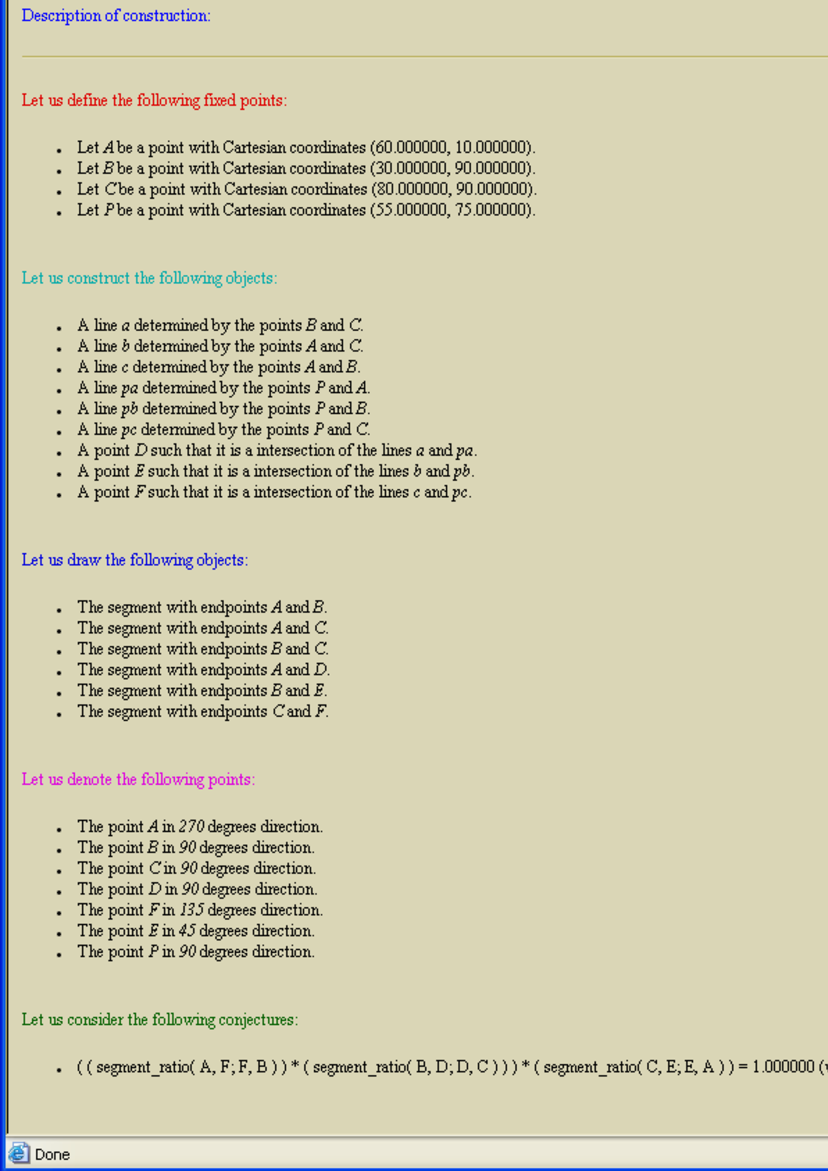
\includegraphics[width=0.5\textwidth]{figures/Figure7.png}
\caption{Natural language presentation of a figure description stored 
in {\sc xml} form}
\label{fig:nl-cons}
\end{center}
\end{figure}


\gclc files can be used for generating figures in {\scshape svg} format:

\begin{itemize}
\item in the command-line version --- using the option \verb|-svg|:
\begin{verbatim}
> gclc example.gcl example.svg -svg
\end{verbatim}

\item in the GUI version of \gclc, by selecting the option 
{\it File/Export to.../SVG}.
\end{itemize}

A picture in {\sc svg} format can be directly open by modern
web browsers.

For \verb|.gcl| files with conjectures, \gclc can generate
proofs in {\sc xml} form:

\begin{itemize}
\item in the command-line version --- if the option \verb|-xmls|
or the option \verb|-svg| is used;
\item in the GUI version of \gclc, by checking the option {\it Source/Generate proof in XML}
or the corresponding button in the source toolbar.
\end{itemize}

\noindent
The {\sc xml} files obtained in the above described way fulfil
restrictions posed by \verb|GeoCons_proof.dtd| (as stated in the
line \verb|<!DOCTYPE figure SYSTEM "GeoCons_proof.dtd">| in each
of these files). For any {\sc xml}, it can be verified if it meets
these restrictions (by analogy with verifying files with constructions).

A {\sc xml} file with a proof contents (valid with respect
to \verb|GeoCons_proof.dtd|) can be converted to a
{\scshape html} form, using \verb|GeoCons_proof.xsl|, for example:
\begin{verbatim}
>AltovaXML.exe /xslt1 GeoCons_proof.xsl /in proof.xml /out proof.html
\end{verbatim}

{\sc xml} files with proofs can be also open directly by web browsers
see one example in the appendix (Section \ref{sec:ceva}).


%----------------------------------------------------------------
\appendix
%----------------------------------------------------------------


%----------------------------------------------------------------
\chapter{List of Errors and Warnings}
%----------------------------------------------------------------


\begin{verbatim}
Syntax error: Number expected.
Syntax error: Two decimal points in number.
Syntax error: Identifier expected.
Syntax error: Identifier or number expected.
Syntax error: Undefined variable.
Syntax error: Wrong variable type.
Syntax error: Symbol '{' expected.
Syntax error: Symbol '}' expected.
Syntax error: Unrecognized definition or command.
Invalid or non-defined expression.
Symbol ';' expected.
Invalid while block.
Invalid if-then-else block.
Invalid procedure definition.
Too many while-block executions (more than 10000). Possible infinite loop.
The conjecture given to prove is ill-formed or includes a point
that is not constructed by commands supported by the prover.
Syntax error: Unknown procedure.
Syntax error: Parameters lists not matched.
Syntax error: Procedures cannot be defined within while-blocks or procedures
Syntax error: Invalid tree description.
Syntax error: Invalid graph description.
Invalid include file.

Input error: Invalid input.

Run-time error: Bad definition. Can not determine line.
Run-time error: Bad definition. Circle radius too small.
Run-time error: Bad definition. Can not determine intersection.
Run-time error: Bad definition. Can not determine angle.
Run-time error: Bad definition. Cannot determine ellipse.
Run-time error: Cannot export data.

Memory error: Cannot allocate enough memory.

Warning: Changing variable value
Warning: Changing variable type
\end{verbatim}


%----------------------------------------------------------------
\chapter{Version History}
%----------------------------------------------------------------

\begin{description}
\item[1995] First version of \gclc;

\item[1996] First public (internet) release of \gclc (\gclc v1.0) ;

\item[1998] \gclc v2.0 : Cartesian commands
(including conics) added. Full vertical compatibility.
\item[2000] \gclc v2.1 : Several bugs fixed.
\item[2003] \gclc v3.0 : Commands

\verb|dim|,

\verb|area|,

\verb|color|,

\verb|drawline|,

\verb|getx|,

\verb|gety|,

\verb|fontsize|,

\verb|animation_frames|,

\verb|trace|

\noindent
added. Full vertical compatibility (for input format). New export format and new
\LaTeX{} style is used (\verb|gclc.sty|). Since this version, commands
\verb|cmark| do not have to precede other drawing commands.

\wingclc --- first release (graphical interface: \copyright{}
2003-2009 Ivan Trajković, Predrag Janičić); only for Windows,
uses Microsoft Foundation Class Library;

\item[2004] \gclc v3.1: Several small bugs fixed.

\index{JavaView}
\wingclc 2004: support for exporting an animation to
a sequence of bitmaps, which can then be used for generating animated
gif (by some other tool) or the animation in some other format. Import
from JavaView \verb|.jvx| format is integrated in \wingclc.


\item[2005] \gclc v4.0:
Commands

\verb|expression|,

\verb|while|,

\verb|random|,

\verb|ang_draw_parametric_curve|,

\verb|ang_drawsystem1|,

\verb|ang_drawsystem_a|,

\verb|ang_drawsystem0_a|,

\verb|ang_drawsystem1_a|

\noindent
added. Full vertical compatibility. A bug in drawing negative arcs fixed.

\wingclc 2005: no changes in the Windows interface.

\item[2006] \gclc v5.0: Theorem prover tightly built-in. Full vertical
compatibility.

The commands

\verb|foot|,

\verb|online|,

\verb|angle_o|,

\verb|drawdashline|

\verb|ang_drawsystem_p|,

\verb|ang_scale|,

\verb|prove|,

\verb|prooflevel|,

\verb|prooflimit|,

\noindent
added. If not defined, \verb|area| (a visible part of the picture)
is, by default, the whole of the picture (which is relevant for
\verb|drawline| and \verb|drawdashline| as they are applied only
if there is defined \verb|area| --- now always).
There is support for colors for \LaTeX{} files, i.e., the command
\verb|color| is relevant for exporting to \LaTeX{} too (not only
for exporting to bitmap). The new manual and the help file.

\wingclc 2006: The behavior of changing line thickness
(by the commands \verb|linethickness|, \verb|normal|, \verb|double|)
is fixed and improved for \wingclc{} and for export to bitmap.
New application icon and new file type icon.


\item[2006] \gclc v6.0: Full vertical compatibility.
Added options for export to {\sc eps} (Encapsulated PostScript) and
{\sc svg}. Full support for {\sc xml} (both for construction descriptions
and proofs). Added options for deductive verification of constructions.

The following commands were added:

\verb|procedure|

\verb|call|

\noindent
(providing support for user-defined procedures),

\verb|ang3d_picture|,

\verb|ang3d_origin|,

\verb|ang3d_unit|,

\verb|ang3d_scale|,

\verb|ang3d_point|,

\verb|ang3d_axes_drawing_range|,

\verb|ang3d_drawline_p|,

\verb|ang3d_drawsystem_p|,

\verb|ang3d_draw_parametric_surface|,

\verb|ang3d_draw_parametric_curve|,

\noindent
(providing support for 3D Cartesian system) and

\verb|drawarc_p|

\verb|dradashwarc_p|

\verb|set_equal|

\verb|printvalueat_rb <p_id> <id>|

\verb|background|

\verb|ang_plot_data|.

For the commands \verb|ang_intersec2|, \verb|bis|, 
\verb|intersec|, \verb|intersec2|, \verb|med|,
\verb|perp|, \verb|sim|, 
full names (\verb|ang_intersection2|, \verb|bisector|,
\verb|intersection|, \verb|intersection2|,
 \verb|mediatrice|, \verb|perpendicular|, 
\verb|symmetrical|) can also be used.

Using the theorem prover is simpler. Instead of stating
conjectures in terms of geometric quantities, one can
also use the following basic sorts of conjectures:
\verb|identical A B|, \verb|collinear A B C|, \verb|perpendicular A B C D|,
\verb|parallel A B C D|, \verb|midpoint O A B|, \verb|same_length A B C D|,
\verb|harmonic A B C D|.

The sequence of commands in while-blocks now shares
both the defined variables and the environment with the outer
context (In previous versions, the environment, defined by commands
\verb|ang_picture| and \verb|ang_origin| etc) was reset in
while-blocks).

In \wingclc{}, there are new icons for easier use of the theorem prover.

In \wingclc{} viewer and bitmap images (as well as in newly
supported formats, {\sc eps} and {\sc svg}) circles and arcs
are not represented by small segments, but by proper circles
and arcs.

\wingclc 2006.1: New icons for easier using of the theorem prover.

When exporting a particular frame from an animation, traces
are also saved to output files.

\item[2007] \gclc 7.0:
Several small fixes were made and the following commands were added:

\verb|drawtree|

\verb|if_then_else|

\wingclc 2007: no changes in the Windows interface.

Support for hyperbolic geometry (through Poincar\'e disc model)
is given via a sample file, as illustration of the mechanism of
user-defined procedures (\verb|sample21_hyp.gcl|).



\item[2007.1] \gclc 7.1:
Several small fixes were made.

Support for arrays (and the command \verb|array|) added.

Support for export to another \LaTeX{} formats ---
PSTricks and Ti{\em k}Z.

Support for including other files (and the command \verb|include|)
added.

Arguments for procedure calls can now also be constants.

If a tree node should not be labelled, its name should start with
the symbol \verb|_| (in the previous version, its name had to be
just the symbol \verb|_|).
All tree nodes introduced by \verb|drawtree| can be used as points.

If there is no defined area for \verb|ang_picture| (or
\verb|ang3d_picture|), the default area is empty.

File exported to vector formats (\LaTeX, {\sc svg}, {\sc xml})
contain comments --- explanations for portions of code for
easier understanding and modifying.

In the command line version, assumed file names are supported.

The batch processing option added.

The following commands were added:

\verb|filltriangle|

\verb|fillrectangle|

\verb|fillcircle|

\verb|fillellipse|

\verb|fillarc|

\verb|fillellipsearc|

\verb|dashstyle|

\verb|drawarrow|

\verb|arrowstyle|

\verb|drawbezier3|

\verb|drawdashbezier3|

\verb|drawbezier4|

\verb|drawdashbezier4|

\verb|bezierprecision|

\verb|drawellipsearc1|

\verb|drawdashellipsearc1|

\verb|drawellipsearc2|

\verb|drawdashellipsearc2|

\verb|rotateonellipse|

\verb|onsegment|

\verb|oncircle|

\verb|mcp|


\wingclc 2007.1: no changes in the Windows interface.


\item[2008] \gclc 8.0:

New theorem provers added: one based on the Wu's method
and one based on the Gr\"obner bases method.

New form of \verb|intersection| command (intersection of lines
determined by the given four points).

The following commands were added:

\verb|prover_timeout|

\verb|theorem_name|

\verb|layer|

\verb|hide_layer|

\verb|hide_layers_from|

\verb|hide_layers_to|

\verb|ang_getx|

\verb|ang_gety|

\verb|ang3d_getx|

\verb|ang3d_gety|

\verb|ang3d_getz|

\verb|fillellipsearc0|

\verb|fillarc0|

Several bugs fixed.

% one-argument function 'abs' again named abs (in v7.2 it was 'fabs')

\wingclc 2008: New buttons added for additional theorem provers.

\item[2008] \gclc 8.1:

The following commands were added:

\verb|drawgraph_a|

\verb|drawgraph_b|

\item[2009] \gclc 9.0:

Several small fixes were made.

The following commands were added:

\verb|getcenter|

\verb|export_to_latex|

\verb|export_to_simple_latex|

\verb|export_to_pstricks|

\verb|export_to_tikz|

\verb|export_to_eps|

\verb|export_to_svg|

New version of support for hyperbolic geometry (through Poincar\'e disc model)
is given via a new version of the sample file \verb|sample21_hyp.gcl|
(co-authored with Zoran Lučić).

\wingclc 2009: no changes in the Windows interface.

\item[2015] A completely new versions of graphical user interfaces for Windows
and Linux, using Qt library. \wingclc is not maintained nor distributed anymore.
Only minor bug-fixes in the engine, vertical compatibility kept.

\item[2020] Code revision, speed-ups, minor bugs fixed, minor changes in 
output in the PSTricks and {\sc svg} formats, and in the output of algebraic
based automated theore provers. The code turns open-source and available on
\verb|github|: \url{https://github.com/janicicpredrag/gclc}.

\item[2022] Minor changes and fixes.

\item[2024] A web-based interface to \gclc released (authored by Nikola Ubavić):
\url{http://www.matf.bg.ac.rs/~janicic/gclc/gclc-web/}. A new \verb|cmake| system
(authored by Matthew Fernandez).
\end{description}


%----------------------------------------------------------------
\chapter{Additional Modules}
%----------------------------------------------------------------


There are several additional modules that going with the basic \gclc
program:

\begin{itemize}
\item \wingclc/\gclcgui: \gclc with graphical user interface.

\label{p:view}
\index{view}
\item Simple previewer {\sc view} for \gclc output files (there
is no need to ``latex'' them) (\copyright{} 1996-2003 Predrag Janičić).
Supports both output formats (old, based on \verb|emlines.sty| and
new, based on \verb|gclc.sty|). A picture \verb|out.pic| generated
by \gclc can be seen by:

\verb|> view out.pic|

Program {\sc view} has the following commands (they are similar to
commands in \TeX{} viewers):

\begin{itemize}
\item {$\rightarrow$} right ;
\item {$\leftarrow$} left ;
\item {$\uparrow$} up ;
\item {$\downarrow$} down ;
\item {$+$} zoom-in ;
\item {$-$} zoom-out ;
\item \verb|C| increase step ;
\item \verb|F| decrease step ;
\item \verb|Q| quit.
\end{itemize}

\index{JavaView}
\item {\sc JavaView} to \gclc converter {\sc jv2gcl} (\copyright{}
2002 Predrag Janičić): converts files from {\sc JavaView} to
\gclc format.\footnote{This program was developed in collaboration
with prof.~Konrad Polthier and Klaus Hildebrandt from Mathematical
Institute, Technical University, Berlin. This work was partially
supported by {\sc daad} grant form my visit to Technical University, Berlin (2003).}
\end{itemize}



%----------------------------------------------------------------
\chapter{Acknowledgements}
%----------------------------------------------------------------


I am grateful to:

\begin{itemize}
\item Prof.~Mirjana Đorić for the initial discussion
which led to the first version of \gclc (1995);

\item Ivan Trajković, the main author of the first version of Windows
graphical interface in \wingclc (2003);

\item Prof.~Neda Bokan and other members of the Group
for geometry, education and visualization with applications
(mostly based at the Faculty of Mathematics, University of Belgrade)
for their invaluable support in developing the \wingclc package (2003);

\item {\sc daad} (Germany) for funding my visit to Konrad Polthier's
group at Mathematical Institute of TU Berlin (2003), which I used for making
a JavaView $\rightarrow$ \gclc converter. I also thank prof.~Konrad Polthier
and Klaus Hildebrandt for their hospitality and their collaboration
in developing this converter;

\item {\sc cim/cisuc} (University of Coimbra, Portugal) for funding my visit to
the Department of Mathematics, University of Coimbra (2005), which I
used for developing the geometry theorem prover built into \gclc. I also
thank prof.~Pedro Quaresma for his warm hospitality and his collaboration
in developing this prover;

\item Prof.~Pedro Quaresma (University of Coimbra), Jelena Tomašević, and
Milena Vujošević-Janičić, coauthors of the {\sc xml} support for \gclc
(2006);

\item Prof.~Bruno Buchberger (RISC, University of Linz, Austria), for
kindly inviting me to visit RISC and to present \gclc there (2006).

\item {\sc emis} (The European Mathematical Information Service) for
mirroring \gclc web page at \url{http://www.emis.de/misc/software/gclc/}
and other {\sc emis} locations.

\item James Fry (New Albany, Indiana, USA) for careful revision of
the \gclc/\-\wingclc manual and help file and for many useful insights
and comments (2005);

\item Goran Predović (University of Belgrade, Serbia and Microsoft
Development Center Belgrade) --- the main author of the theorem provers
based on the Wu's method and Gr\"obner based method (2008).

\item Luka Tomašević (University of Belgrade, Serbia) --- the
main author of the support for graph drawing (2008).

\item Nikola Ubavić (University of Belgrade, Serbia) --
the author of the web-based version of GCLC (2024);

\item Matthew Fernandez (USA) --- the author of the CMAKE system,
also for improving different parts of the GCLC code.

\item Prof.~Stefano Marchiafava (University ,,La Sapienza``, Rome, Italy), for kindly
inviting me to visit the University ,,La Sapienza`` and to present \gclc there (2008).

\item Colleagues who gave useful comments and certain contributions and 
influenced development of \gclc: Nenad Dedić, Miloš
Utvić, Nikola Begović, Ivan Elčić, Jelena Grmuša,
Aleksandra Nenadić, Marijana Lukić, Srđan Vukmirović,
Goran Terzić, Milica Labus, Aleksandar Gogić, Aleksandar
Samardžić, Ivan Čukić, Nikola Ubavić (1999/2022);

\item Konrad Polthier (TU Berlin), Zach (Temple University, USA),
Vladimir Baltić (University of Belgrade), Hristos Bitos (Greece),
Aleksandar Gogić (DTA, Belgrade), Bob Schumacher (Cedarville
University, Ohio, USA), Pedro Quaresma (University of Coimbra,
Portugal), Zoran Lučić (University of Belgrade), Biljana
Radovanović (University of Belgrade), Nedeljko Stefanović
(University of Belgrade), Milan Mitrović (Slovenia), Thomas
Speziale (USA), Ania Piktas (Poland), Bojan Radusinović (Serbia),
Pierre Larochelle (Florida Institute of Technology, USA),
Robert Hartmann (TU Clausthal, Clausthal-Zellerfeld, Germany), and
Xavier Allamigeon for useful feedback and suggestions on different
versions of \gclc/\wingclc.

\item All \gclc users for their support, feedback and
suggestions.
\end{itemize}


%----------------------------------------------------------------
\chapter{Examples}
%----------------------------------------------------------------

%----------------------------------------------------------------
\section{Example (Simple Triangle)}
%----------------------------------------------------------------


\begin{verbatim}
point A 50 45
point B 45 15
point C 90 15

cmark_lt A
cmark_lb B
cmark_rb C

drawsegment A B
drawsegment B C
drawsegment C A

med a C B
med b A C
intersec O a b
drawcircle O A
\end{verbatim}
\vspace*{-5mm}

\begin{figure}[ht]
\framebox[122mm][l]
{
\begin{minipage}[t]{120mm}
\vspace*{-1mm}
\input{figures/sample0-triangle.tkz}
\end{minipage}
}
\vspace*{-4mm}
%\caption{Output for Example A}
\label{output-example1}
\end{figure}

\newpage


%----------------------------------------------------------------
\section{Example (Conics)}
%----------------------------------------------------------------

\begin{verbatim}
ang_picture 0 0 80 80
ang_origin 20.0 35.0
ang_drawsystem

ang_conic h 0 0 1 -1 0 -3

ang_conicprecision 75

ang_point A1 2 2
ang_point A2 3 2
line l A1 A2
ang_intersec2 P P2 h l

cmark_t P
ang_tangent p P h
color 32 192 32
ang_drawline p
color 32 32 192
ang_drawconic h
color 0 0 0

% --------------------------------------------------

ang_unit 5
ang_picture 85 5 140 100
ang_origin 115.0 45.0
ang_drawsystem

ang_conic h -1 0.5 1 -1 0 -3

ang_conicprecision 50

ang_point A1 2 2
ang_point A2 3 2
line l A1 A2
ang_intersec2 P P2 h l

cmark_t P
ang_tangent p P h
color 32 192 32
ang_drawline p
color 192 32 32
ang_drawdashconic h
\end{verbatim}

\newpage

\begin{figure}[ht]
\framebox[122mm][l]
{
\begin{minipage}[t]{120mm}
\gclcpicture{1}
\input{figures/sample-conics.tkz}
\end{minipage}
}
%\caption{Output for Example C}
\label{output-example3}
\end{figure}


\newpage

%----------------------------------------------------------------
\section{Example (Parametric Curves)}
%----------------------------------------------------------------

\begin{verbatim}
ang_picture 5 5 112 92
ang_origin 45 35
ang_drawsystem_a

point X -0.5 0 0.5 0
point O 0 0
distance d X O

color 255 0 0
ang_draw_parametric_curve x {-3;x<8;x+0.1}{x;d/x}

color 0 0 255
ang_draw_parametric_curve x {-3;x<8;x+0.1}{x;d*x*sin(10*d*x)}

color 100 200 100
ang_draw_parametric_curve t {0;t<30;t+0.3}{sin(d*t)*t/6;-cos(d*t)*t/6}

animation_frames 50 5
\end{verbatim}

\newpage

\begin{figure}[ht]
\framebox[122mm][l]
{
\begin{minipage}[t]{120mm}
\gclcpicture{1}
\input{figures/sample-curves.tkz}
\end{minipage}
}
%\caption{Output for Example D}
\label{output-example4}
\end{figure}

\newpage


%----------------------------------------------------------------
\section{Example (While-loop)}
%----------------------------------------------------------------

\begin{verbatim}
dim 120 80

ang_picture 5 5 115 70
ang_origin 45 25
ang_drawsystem_a

ang_draw_parametric_curve x {-3;x<5;x+0.05}{x;0.3*x*sin(3*x)}

% while loop in conjunction with parametric curves
number x -3
while { x<5 }
{
    ang_picture 10 10 100 70
    ang_origin 45 25

    expression y { 0.3*x*sin(3*x) }
    ang_point A x 0
    ang_point B x y
    drawsegment A B

    expression x { x+0.05}
}
\end{verbatim}



\newpage

\begin{figure}[ht]
\framebox[122mm][l]
{
\begin{minipage}[t]{120mm}
\gclcpicture{1}
\input{figures/sample-while.tkz}
\end{minipage}
}
%\caption{Output for Example D}
%\label{output-example4}
\end{figure}

\newpage


%----------------------------------------------------------------
\section{Example (Ceva's theorem)}
\label{sec:ceva}
%----------------------------------------------------------------

\begin{verbatim}
point A 30 10
point B 80 10
point C 60 90
point P 55 55

line a B C
line b A C
line c A B

line pa P A
line pb P B
line pc P C

intersec D a pa
intersec E b pb
intersec F c pc

drawsegment A B
drawsegment A C
drawsegment B C

drawsegment A D
drawsegment B E
drawsegment C F

cmark_b A
cmark_b B
cmark_t C
cmark_rt D
cmark_b F
cmark_lt E
cmark_r P

prove { equal { mult { mult { sratio A F F B }
                            { sratio B D D C } }
                     { sratio C E E A } }
              1 }
\end{verbatim}


\begin{figure}[ht]
\framebox[122mm][l]
{
\begin{minipage}[t]{120mm}
\gclcpicture{1}
\input{figures/sample_ceva.tkz}
\end{minipage}
\vspace*{-2cm}
}
\caption{Output for Example E}
\label{output-example5}
\end{figure}


\newpage

\LaTeX{} output of the prover based on the area method:
\vspace*{5mm}


\begin{longtable}{llll}
\proofstep{ \left( \left( \frac{\overrightarrow{AF}}{\overrightarrow{FB}} \cdot  \frac{\overrightarrow{BD}}{\overrightarrow{DC}}\right) \cdot  \frac{\overrightarrow{CE}}{\overrightarrow{EA}}\right)}{=}{ 1 }{by the statement (value 1=1)}
\proofstep{ \left( \left( \left( -1  \cdot  \frac{\overrightarrow{AF}}{\overrightarrow{BF}}\right) \cdot  \frac{\overrightarrow{BD}}{\overrightarrow{DC}}\right) \cdot  \frac{\overrightarrow{CE}}{\overrightarrow{EA}}\right)}{=}{ 1 }{by geometric simplifications (value 1=1)}
\proofstep{ \left( -1  \cdot  \left( \frac{\overrightarrow{AF}}{\overrightarrow{BF}} \cdot  \left( \frac{\overrightarrow{BD}}{\overrightarrow{DC}} \cdot  \frac{\overrightarrow{CE}}{\overrightarrow{EA}}\right)\right)\right)}{=}{ 1 }{by algebraic simplifications (value 1=1)}
\proofstep{ \left( -1  \cdot  \left( \frac{ S_{APC}}{ S_{BPC}} \cdot  \left( \frac{\overrightarrow{BD}}{\overrightarrow{DC}} \cdot  \frac{\overrightarrow{CE}}{\overrightarrow{EA}}\right)\right)\right)}{=}{ 1 }{by Lemma 8 (point $F$ eliminated) (value 1=1)}
\proofstep{ \left( -1  \cdot  \left( \frac{ S_{APC}}{ S_{BPC}} \cdot  \left( \frac{\overrightarrow{BD}}{\overrightarrow{DC}} \cdot  \left( -1  \cdot  \frac{\overrightarrow{CE}}{\overrightarrow{AE}}\right)\right)\right)\right)}{=}{ 1 }{by geometric simplifications (value 1=1)}
\proofstep{ \frac{ \left( S_{APC} \cdot  \left( \frac{\overrightarrow{BD}}{\overrightarrow{DC}} \cdot  \frac{\overrightarrow{CE}}{\overrightarrow{AE}}\right)\right)}{ S_{BPC}}}{=}{ 1 }{by algebraic simplifications (value 1=1)}
\proofstep{ \frac{ \left( S_{APC} \cdot  \left( \frac{\overrightarrow{BD}}{\overrightarrow{DC}} \cdot  \frac{ S_{CPB}}{ S_{APB}}\right)\right)}{ S_{BPC}}}{=}{ 1 }{by Lemma 8 (point $E$ eliminated) (value 1=1)}
\proofstep{ \frac{ \left( S_{APC} \cdot  \left( \left( -1  \cdot  \frac{\overrightarrow{BD}}{\overrightarrow{CD}}\right) \cdot  \frac{ S_{CPB}}{ S_{APB}}\right)\right)}{ \left( -1  \cdot  S_{CPB}\right)}}{=}{ 1 }{by geometric simplifications (value 1=1)}
\proofstep{ \frac{ \left( S_{APC} \cdot  \frac{\overrightarrow{BD}}{\overrightarrow{CD}}\right)}{ S_{APB}}}{=}{ 1 }{by algebraic simplifications (value 1=1)}
\proofstep{ \frac{ \left( S_{APC} \cdot  \frac{ S_{BPA}}{ S_{CPA}}\right)}{ S_{APB}}}{=}{ 1 }{by Lemma 8 (point $D$ eliminated) (value 1=1)}
\proofstep{ \frac{ \left( S_{APC} \cdot  \frac{ S_{BPA}}{ \left( -1  \cdot  S_{APC}\right)}\right)}{ \left( -1  \cdot  S_{BPA}\right)}}{=}{ 1 }{by geometric simplifications (value 1=1)}
\proofstep{ 1 }{=}{ 1 }{by algebraic simplifications (value 1=1)}
\end{longtable}

\vspace*{2mm} \hrule \vspace*{2mm}


\centerline{Q.E.D.}



NDG conditions are:

$ S_{BPA}\neq S_{CPA}$ i.e., lines $BC$ and $PA$ are not parallel (construction based assumption)

$ S_{APB}\neq S_{CPB}$ i.e., lines $AC$ and $PB$ are not parallel (construction based assumption)

$ S_{APC}\neq S_{BPC}$ i.e., lines $AB$ and $PC$ are not parallel (construction based assumption)

$ P_{FBF}\neq 0 $ i.e., points $F$ and $B$ are not identical (conjecture based assumption)

$ P_{DCD}\neq 0 $ i.e., points $D$ and $C$ are not identical (conjecture based assumption)

$ P_{EAE}\neq 0 $ i.e., points $E$ and $A$ are not identical (conjecture based assumption)


\vspace*{2mm} \hrule \vspace*{2mm}


Number of elimination proof steps:      3

Number of geometric proof steps:        6

Number of algebraic proof steps:       23

Total number of proof steps:           32


Time spent by the prover: 0.002 seconds
\vspace*{1cm}


A fragment of the {\sc xml} output of the prover based on the area method:

\begin{figure}[ht]
\begin{center}
\hspace*{-5cm}
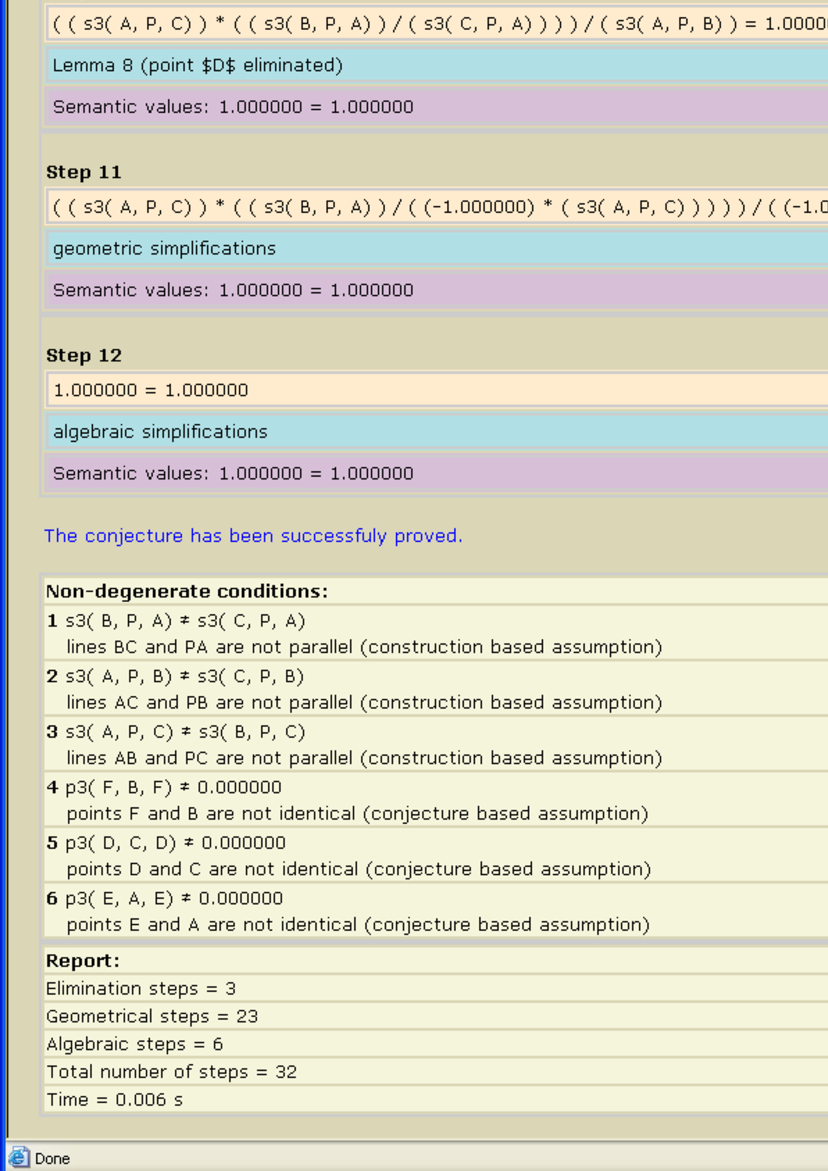
\includegraphics[width=0.4\textwidth]{figures/Figure8.png}
\end{center}
\end{figure}


A fragment of the \LaTeX{} output of the prover based on the Wu's method:


\subsection*{Creating polynomials from hypotheses}

\begin{itemize}

\item Point $A$

no condition

\item Point $B$

no condition

\item Point $C$

no condition

\item Point $P$

no condition

\item Line $a$: $B$ $C$

\begin{itemize}
\item point $B$ is on the line ($B$, $C$)

no condition

\item point $C$ is on the line ($B$, $C$)

no condition
\end{itemize}

\item Line $b$: $A$ $C$

\begin{itemize}
\item point $A$ is on the line ($A$, $C$)

no condition

\item point $C$ is on the line ($A$, $C$)

no condition
\end{itemize}

\item Line $c$: $A$ $B$

\begin{itemize}
\item point $A$ is on the line ($A$, $B$)

no condition

\item point $B$ is on the line ($A$, $B$)

no condition
\end{itemize}

\item Line $pa$: $P$ $A$
\begin{itemize}

\item point $P$ is on the line ($P$, $A$)

no condition

\item point $A$ is on the line ($P$, $A$)

no condition

\end{itemize}
\item Line $pb$: $P$ $B$
\begin{itemize}

\item point $P$ is on the line ($P$, $B$)

no condition

\item point $B$ is on the line ($P$, $B$)

no condition
\end{itemize}

\item Line $pc$: $P$ $C$

\begin{itemize}
\item point $P$ is on the line ($P$, $C$)

no condition

\item point $C$ is on the line ($P$, $C$)

no condition
\end{itemize}

\item Intersection of lines, $D$: $a$ $pa$

\begin{itemize}
\item point $D$ is on the line ($B$, $C$)
$$p_{33}  =  -u_{3}x_{2}+(u_{2}-u_{1})x_{1}+u_{3}u_{1}$$
\item point $D$ is on the line ($P$, $A$)
$$p_{34}  =  u_{5}x_{2}-u_{4}x_{1}$$
\end{itemize}

\item Intersection of lines, $E$: $b$ $pb$
\begin{itemize}
\item point $E$ is on the line ($A$, $C$)
$$p_{35}  =  -u_{3}x_{4}+u_{2}x_{3}$$
\item point $E$ is on the line ($P$, $B$)
$$p_{36}  =  u_{5}x_{4}+(-u_{4}+u_{1})x_{3}-u_{5}u_{1}$$
\end{itemize}

\item Intersection of lines, $F$: $c$ $pc$

\begin{itemize}
\item point $F$ is on the line ($A$, $B$)
 --- true by the construction

no condition

\item point $F$ is on the line ($P$, $C$)
$$p_{37}  =  (u_{5}-u_{3})x_{6}+(-u_{5}u_{2}+u_{4}u_{3})$$
\end{itemize}
\end{itemize}

\subsection*{Creating polynomial from the conjecture}

\begin{itemize}
\item Processing given conjecture(s).
\end{itemize}

\begin{description}
\item [Conjecture 1:]
$$p_{38}  =  -2x_{6}x_{3}x_{1}+u_{3}x_{6}x_{3}+u_{3}x_{6}x_{1}+u_{1}x_{3}x_{1}-u_{3}u_{1}x_{3}$$
\end{description}


\subsection*{Invoking the theorem prover}

The used proving method is Wu's method.

The input system is:

\begin{eqnarray*}
p_{0} &=& -u_{3}x_{2}+(u_{2}-u_{1})x_{1}+u_{3}u_{1}\\
p_{1} &=& u_{5}x_{2}-u_{4}x_{1}\\
p_{2} &=& -u_{3}x_{4}+u_{2}x_{3}\\
p_{3} &=& u_{5}x_{4}+(-u_{4}+u_{1})x_{3}-u_{5}u_{1}\\
p_{4} &=& (u_{5}-u_{3})x_{6}+(-u_{5}u_{2}+u_{4}u_{3})\\
\end{eqnarray*}


\subsubsection*{Triangulation, step 1}

\begin{description}
\item [Choosing variable:]  Trying the variable with index 6.
\item [Variable $x_{6}$ selected:]  The number of polynomials with this variable is 1.
\item [Single polynomial with chosen variable:]  No reduction needed.
\item The triangular system has not been changed.
\end{description}


\subsubsection*{Triangulation, step 2}

\begin{description}
\item [Choosing variable:]  Trying the variable with index 5.
\item [Choosing variable:]  Trying the variable with index 4.
\item [Variable $x_{4}$ selected:]  The number of polynomials with this variable is 2.
\item [Minimal degrees:]  3 polynomials with degree 1 and 2 polynomials with degree 1.
\item [Polynomial with linear degree:]  Removing variable $x_{4}$ from all other polynomials by reducing them with polynomial $p_{3}$.
\end{description}

Finished a triangulation step, the current system is:

\begin{eqnarray*}
p_{0} &=& -u_{3}x_{2}+(u_{2}-u_{1})x_{1}+u_{3}u_{1}\\
p_{1} &=& u_{5}x_{2}-u_{4}x_{1}\\
p_{2} &=& (u_{5}u_{2}-u_{4}u_{3}+u_{3}u_{1})x_{3}-u_{5}u_{3}u_{1}\\
p_{3} &=& u_{5}x_{4}+(-u_{4}+u_{1})x_{3}-u_{5}u_{1}\\
p_{4} &=& (u_{5}-u_{3})x_{6}+(-u_{5}u_{2}+u_{4}u_{3})\\
\end{eqnarray*}


\subsubsection*{Triangulation, step 3}

\begin{description}
\item [Choosing variable:]  Trying the variable with index 3.
\item [Variable $x_{3}$ selected:]  The number of polynomials with this variable is 1.
\item [Single polynomial with chosen variable:]  No reduction needed.
\item The triangular system has not been changed.
\end{description}


\subsubsection*{Triangulation, step 4}

\begin{description}
\item [Choosing variable:]  Trying the variable with index 2.
\item [Variable $x_{2}$ selected:]  The number of polynomials with this variable is 2.
\item [Minimal degrees:]  1 polynomials with degree 1 and 0 polynomials with degree 1.
\item [Polynomial with linear degree:]  Removing variable $x_{2}$ from all other polynomials by reducing them with polynomial $p_{1}$.
\end{description}

Finished a triangulation step, the current system is:

\begin{eqnarray*}
p_{0} &=& (u_{5}u_{2}-u_{5}u_{1}-u_{4}u_{3})x_{1}+u_{5}u_{3}u_{1}\\
p_{1} &=& u_{5}x_{2}-u_{4}x_{1}\\
p_{2} &=& (u_{5}u_{2}-u_{4}u_{3}+u_{3}u_{1})x_{3}-u_{5}u_{3}u_{1}\\
p_{3} &=& u_{5}x_{4}+(-u_{4}+u_{1})x_{3}-u_{5}u_{1}\\
p_{4} &=& (u_{5}-u_{3})x_{6}+(-u_{5}u_{2}+u_{4}u_{3})\\
\end{eqnarray*}


\subsubsection*{Triangulation, step 5}

\begin{description}
\item [Choosing variable:]  Trying the variable with index 1.
\item [Variable $x_{1}$ selected:]  The number of polynomials with this variable is 1.
\item [Single polynomial with chosen variable:]  No reduction needed.
\item The triangular system has not been changed.
\end{description}

The triangular system is:

\begin{eqnarray*}
p_{0} &=& (u_{5}u_{2}-u_{5}u_{1}-u_{4}u_{3})x_{1}+u_{5}u_{3}u_{1}\\
p_{1} &=& u_{5}x_{2}-u_{4}x_{1}\\
p_{2} &=& (u_{5}u_{2}-u_{4}u_{3}+u_{3}u_{1})x_{3}-u_{5}u_{3}u_{1}\\
p_{3} &=& u_{5}x_{4}+(-u_{4}+u_{1})x_{3}-u_{5}u_{1}\\
p_{4} &=& (u_{5}-u_{3})x_{6}+(-u_{5}u_{2}+u_{4}u_{3})\\
\end{eqnarray*}


\subsection*{Final remainder}


\subsubsection*{Final remainder for conjecture 1}

Calculating final remainder of the conclusion:
$$g  =  -2x_{6}x_{3}x_{1}+u_{3}x_{6}x_{3}+u_{3}x_{6}x_{1}+u_{1}x_{3}x_{1}-u_{3}u_{1}x_{3}$$
with respect to the triangular system.

\begin{enumerate}
\item Pseudo remainder with $p_{4}$ over variable $x_{6}$:
$$g  =  (-2u_{5}u_{2}+u_{5}u_{1}+2u_{4}u_{3}-u_{3}u_{1})x_{3}x_{1}+$$
$$(u_{5}u_{3}u_{2}-u_{5}u_{3}u_{1}-u_{4}u_{3}^{2}+u_{3}^{2}u_{1})x_{3}+(u_{5}u_{3}u_{2}-u_{4}u_{3}^{2})x_{1}$$
\item Pseudo remainder with $p_{3}$ over variable $x_{4}$:
$$g  =  (-2u_{5}u_{2}+u_{5}u_{1}+2u_{4}u_{3}-u_{3}u_{1})x_{3}x_{1}+$$
$$(u_{5}u_{3}u_{2}-u_{5}u_{3}u_{1}-u_{4}u_{3}^{2}+u_{3}^{2}u_{1})x_{3}+(u_{5}u_{3}u_{2}-u_{4}u_{3}^{2})x_{1}$$

\item Pseudo remainder with $p_{2}$ over variable $x_{3}$:
$$g  =  (u_{5}^{2}u_{3}u_{2}^{2}-2u_{5}^{2}u_{3}u_{2}u_{1}+u_{5}^{2}u_{3}u_{1}^{2}-2u_{5}u_{4}u_{3}^{2}u_{2}+$$
$$2u_{5}u_{4}u_{3}^{2}u_{1}+u_{5}u_{3}^{2}u_{2}u_{1}-u_{5}u_{3}^{2}u_{1}^{2}+u_{4}^{2}u_{3}^{3}-u_{4}u_{3}^{3}u_{1})x_{1}+$$
$$(u_{5}^{2}u_{3}^{2}u_{2}u_{1}-u_{5}^{2}u_{3}^{2}u_{1}^{2}-u_{5}u_{4}u_{3}^{3}u_{1}+u_{5}u_{3}^{3}u_{1}^{2})$$

\item Pseudo remainder with $p_{1}$ over variable $x_{2}$:
$$g  =  (u_{5}^{2}u_{3}u_{2}^{2}-2u_{5}^{2}u_{3}u_{2}u_{1}+u_{5}^{2}u_{3}u_{1}^{2}-2u_{5}u_{4}u_{3}^{2}u_{2}+$$
$$2u_{5}u_{4}u_{3}^{2}u_{1}+u_{5}u_{3}^{2}u_{2}u_{1}-u_{5}u_{3}^{2}u_{1}^{2}+u_{4}^{2}u_{3}^{3}-u_{4}u_{3}^{3}u_{1})x_{1}+$$
$$(u_{5}^{2}u_{3}^{2}u_{2}u_{1}-u_{5}^{2}u_{3}^{2}u_{1}^{2}-u_{5}u_{4}u_{3}^{3}u_{1}+u_{5}u_{3}^{3}u_{1}^{2})$$

\item Pseudo remainder with $p_{0}$ over variable $x_{1}$:
$$g  =  0$$
\end{enumerate}


\subsection*{Prover report}

\begin{description}
\item [Status:]  The conjecture has been proved.
\item [Space Complexity:]  The biggest polynomial obtained during proof process contained 13 terms.
\item [Time Complexity:]  Time spent by the prover is 0.053 seconds.
\item[NDG conditions] are:

\begin{itemize}
\item
$ P_{FBF}\neq 0 $ i.e., points $F$ and $B$ are not identical (conjecture based assumption).
\item
$ P_{DCD}\neq 0 $ i.e., points $D$ and $C$ are not identical (conjecture based assumption).
\item
$ P_{EAE}\neq 0 $ i.e., points $E$ and $A$ are not identical (conjecture based assumption).
\end{itemize}
\end{description}



%\bibliography{...}
%\bibliographystyle{abbrv}

\begin{thebibliography}{10}

\bibitem{buchbergerPhd}
B.~Buchberger.
\newblock {\em An Algorithm for finding a basis for the residue class ring of a
  zero-dimensional polynomial ideal}.
\newblock PhD thesis, Math. Inst. University of Innsbruck, Austria, 1965.

\bibitem{groebner_bases_and_applications}
B.~Buchberger and F.~Winkler, editors.
\newblock {\em Gr\"obner Bases and Applications}.
\newblock Cambridge University Press, 1998.

\bibitem{chou}
S.-C. Chou.
\newblock {\em Mechanical Geometry Theorem Proving}.
\newblock D.Reidel Publishing Company, Dordrecht, 1988.

\bibitem{Chou93}
S.-C. Chou, X.-S. Gao, and J.-Z. Zhang.
\newblock Automated production of traditional proofs for constructive geometry
  theorems.
\newblock In M.~Vardi, editor, {\em Proceedings of the Eighth Annual IEEE
  Symposium on Logic in Computer Science {LICS}}, pages 48--56. IEEE Computer
  Society Press, June 1993.

\bibitem{constructions-teamat}
M.~Đorić and P.~Janičić.
\newblock {Constructions, instructions, interactions }.
\newblock {\em {Teaching Mathematics and its Applications}}, 23(2):69--88,
  2004.

\bibitem{gclc}
P.~Janičić.
\newblock {GCLC -- A Tool for Constructive Euclidean Geometry and More than
  That}.
\newblock In N.~Takayama, A.~Iglesias, and J.~Gutierrez, editors, {\em
  Proceedings of International Congress of Mathematical Software (ICMS 2006)},
  volume 4151 of {\em Lecture Notes in Computer Science}, pages 58--73.
  Springer-Verlag, 2006.

\bibitem{gclc-ijcar}
P.~Janičić and P.~Quaresma.
\newblock {System description: Gclcprover + GeoThms}.
\newblock In U.~Furbach and N.~Shankar, editors, {\em International Joint
  Conference on Automated Reasoning (IJCAR-2006)}, volume 4130 of {\em Lecture
  Notes in Artificial Intelligence}, pages 145--150. Springer-Verlag, 2006.

\bibitem{gclc-jar}
P.~Janičić.
\newblock {Geometry Constructions Language}.
\newblock {\em Journal of Automated Reasoning}, 44(1-2):3--24, 2010.

\bibitem{wingclc}
P.~Janičić and I.~Trajković.
\newblock {WinGCLC --- a Workbench for Formally Describing Figures}.
\newblock In {\em {Proceedings of the 19 mth Spring Conference on Computer
  Graphics (SCCG 2003)}}, pages 251--256, Budmerice, Slovakia, April, 24-26
  2003. ACM Press, New York, USA.

\bibitem{gclc-mkm}
P.~Quaresma and P.~Janičić.
\newblock Integrating dynamic geometry software, deduction systems, and theorem
  repositories.
\newblock In J.~Borwein and W.~Farmer, editors, {\em Mathematical Knowledge
  Management (MKM-2006)}, volume 4108 of {\em Lecture Notes in Artificial
  Intelligence}, pages 280--294. Springer-Verlag, 2006.

\bibitem{Quaresma06}
P.~Quaresma and P.~Janičić.
\newblock {Framework for the Constructive Geometry}.
\newblock Technical Report TR2006/001, Center for Informatics and Systems of
  the University of Coimbra, 2006.

\bibitem{wu1978}
W.-T. Wu.
\newblock On the decision problem and the mechanization of theorem proving in
  elementary geometry.
\newblock {\em Scientia Sinica}, 21:157--179, 1978.

\end{thebibliography}

\printindex


\end{document}
